
\documentclass{article}
\usepackage{fullpage}
\usepackage{amsmath,amssymb}
\usepackage{amsthm}
\usepackage{algorithm,algorithmic}
\usepackage{graphicx}
\usepackage{relsize}
\usepackage{tabu}
\usepackage{booktabs}% for better rules in the table




\numberwithin{equation}{section}
\newtheorem{theorem}{Theorem}[subsection]
\newtheorem{lemma}[theorem]{Lemma}
\newtheorem{proposition}[theorem]{Proposition}
\newtheorem{corollary}[theorem]{Corollary}
% Definition Styles
\theoremstyle{definition}
\newtheorem{definition}[theorem]{Definition}
\newtheorem{example}[theorem]{Example}
\newtheorem{remark}[theorem]{Remark}
\newtheorem*{convention}{Convention}
\newtheorem{compositionlaw}[theorem]{Composition Law}
\newtheorem{alg}[theorem]{Algorithm}
\newtheorem*{DFproblem}{Elliptic Curve Diffie-Hellman Problem}


\renewcommand{\algorithmicrequire}{\textbf{Input:}}
\renewcommand{\algorithmicensure}{\textbf{Output:}}

\newcommand{\CC}{{\mathbb C}} % the set of complex numbers
\newcommand{\NN}{{\mathbb N}} % the set of natural numbers
\newcommand{\QQ}{{\mathbb Q}} % the set of rational numbers
\newcommand{\ZZ}{{\mathbb Z}} % the set of integer numbers
\newcommand{\RR}{{\mathbb R}} % the set of real numbers
\newcommand{\Zmod}[1]{\ZZ / #1\ZZ} % the integers mod n
\newcommand{\FF}[1]{{\mathbb F}_{#1}} % the finite field with q elements
\newcommand{\FFCL}[1]{{\bar {\mathbb F}}_{#1}} % the algebraic closure of a finite field with q elements
\newcommand{\bstring}{\Sigma} % the set of binary strings
\newcommand{\grgen}[1]{\langle #1 \rangle} % the group generated by P
\newcommand{\Char}[1]{\operatorname{char} (#1)} % the character of a field
\newcommand{\proj}[1]{{\mathbb P}^{#1}} % the Projective n-space
\newcommand{\Div}{\operatorname{Div}} % the divisor group of a curve
\newcommand{\Pic}{\operatorname{Pic}} % the divisor class group of a curve
\newcommand{\Enonsing}{E_{\operatorname{ns}}} % the non singular part of and elliptic curve E
\newcommand{\frob}[1][]{\varphi_{#1}} % the Frobenius morphism
\newcommand{\degree}[1]{\operatorname{deg} \left(#1\right)} % the degree of an isogeny
\newcommand{\idegree}[1]{\operatorname{deg}_i \left(#1\right)} % the inseparable degree of an isogeny
\newcommand{\sdegree}[1]{\operatorname{deg}_s \left(#1\right)} % the separable degree of an isogeny
\newcommand{\detm}[1]{\operatorname{det} \left(#1\right)} % the determinant of a matrix
\newcommand{\tr}[1]{\operatorname{tr} \left(#1\right)} % the trace of a matrix
\newcommand{\kernel}[1]{\operatorname{ker} \left(#1\right)} % the kernel of a morphism
\newcommand{\image}[1]{\operatorname{im} \left(#1\right)} % the image of a morphism
\newcommand{\Endring}[1]{\operatorname{End} (#1)} % the endomorphism ring of an elliptic curve
\newcommand{\Endringk}[2]{\operatorname{End}_{#2} (#1)} % the endomorphism ring of an elliptic curve over K
\newcommand{\Autgrp}[1]{\operatorname{Aut} (#1)} % the automorphism group of an elliptic curve
\newcommand{\Autgrpk}[2]{\operatorname{Aut}_{#2} (#1)} % the automorphism group of an elliptic curve over K
\newcommand{\invlim}[1]{\underset{#1}{\varprojlim}} % the inverse limit over all n
\newcommand{\rou}[1]{\boldsymbol{\mu}_{#1}} % the set of m'th roots of unity
\newcommand{\leg}[2]{\left( \frac{#1}{#2}\right)} % the Legendre symbol
\newcommand{\lcm}{\operatorname{lcm}} % the least common multiple of two integers





\begin{document}


\begin{titlepage}
\begin{center}


\includegraphics[width5cm, height=5cm]{unilogo}
\\[1cm]
\textsc{\large Master's thesis in Mathematics} \\[0.5cm]
\hline \\[0.8cm]

{\LARGE \textbf{The use of elliptic curves in cryptography}}\\[0.5cm]
by\\[0.2cm]
{\large Gijsbert van Vliet}
\vfill
{\large Nijmegen, June 2015}\\[2cm]
{\large Supervisors:}\\[0.2cm]
{\large Prof. dr. B.J.J. Moonen}\\
{\large Dr. W. Bosma}
\end{center}
\end{titlepage}
\null\thispagestyle{empty}\newpage

{\LARGE \textbf{Acknowledgements}}\\[1cm]
First of all I would like to express my sincerest gratitude to my supervisor prof. dr. Ben Moonen for all his support throughout the learning process of this master's thesis. Without his patience, encouragement and all insightful conversations we shared, this thesis would have never been completed. Also I would like to thank dr. Wieb Bosma for putting so much of his precious time into helping me and for providing numerous useful remarks. \par 
Furthermore I would like to thank my family and loved ones, who supported me throughout the entire process, both financially and emotionally. Special thanks goes out to my father, Frans van Vliet. He always supported my dreams and aspirations and, if I say so myself, did a fine job raising me. Without him I would have never started this study, let alone finish it. 

\newpage
\tableofcontents
\newpage

\section*{Introduction}
Elliptic curves have been a subject of research for a long time. They naturally occur in the study of Diophantine equations as well as the study of certain complex line integrals, e.g., complex integrals of the form $$ \int d\;t/\sqrt{t(t-1)(t-\lambda)}, $$ which arise when one attempts to compute the arc length of an ellipse. In fact, this is where elliptic curves originally acquired their name from. Around the year 1985 elliptic curves over finite fields, which at first seem to have the structure of rather boring abelian groups, found a new application in cryptography. At that time, discrete logarithm based cryptosystems already played an important role in cryptography. In short, these systems rely on the supposed `hardness' of the \emph{discrete logarithm problem} for abelian groups. The discrete logarithm problem is the problem of, given a finite abelian group $(G,\oplus)$, a point $P\in G$ and a point $Q\in\grgen{P}$, finding an integer $k$ such that $[k]P=Q$, i.e., such that $\underbrace{P\oplus \ldots \oplus P}_{k \text{ times}}=Q$. Victor S. Miller \cite{Miller} and Neal Koblitz \cite{Koblitz} independently realized that using elliptic curves as groups for these systems might be more efficient than the conventional groups, used at that time. They figured that using elliptic curves in cryptosystems could reduce key sizes, while retaining a similar level of security. However, not all elliptic curves are suitable for cryptography, since in some cases the internal structure of an elliptic curve can be used to solve the discrete logarithm problem efficiently.\par  
The main question of this thesis is:
\begin{center} 
\emph{What requirements does an elliptic curve need to meet in order to be considered `safe for cryptographic purposes'?}
\end{center}
In order to answer this question, first elliptic curves have to be defined and their basic properties explained. After that I will explain which requirements an elliptic curve should have in order to provide security for discrete logarithm based cryptosystems and why these requirements have to be met. In short, this thesis consists of the following three parts:
\begin{description}
\item[Part 1:] This part consists only of chapter \ref{cryptointroduction}. In this chapter I will give a short introduction to the subject of cryptography and the role of the discrete logarithm problem in this subject.
\item[Part 2:] The second part of this thesis consists of chapters \ref{ellipticcurvesection} to \ref{schoofsalgorithm}. In this part I will define elliptic curves and give its basic arithmetic properties. Chapter \ref{ellipticcurvesection} will give the basic properties of elliptic curves over arbitrary algebraically closed fields, while chapter \ref{ellipticcurvesoverffsection} will deal with elliptic curves over finite fields. In section \ref{schoofsalgorithm} an algorithm will be given that computes the most important quantity of elliptic curves over finite fields, i.e., its number of rational points. 
\item[Part 3:] In the last part I will focus on the role of elliptic curves in cryptography. First, in chapter \ref{protocols}, I will give a few explicit examples of how elliptic curves can be used in cryptography. After that I will explain the most important attacks on the discrete logarithm problem. These include attacks on the discrete logarithm problem for general groups in chapter \ref{generalattacksonDLP} and three attacks on this problem for certain specific elliptic curves in chapter \ref{MOV} to \ref{Anomalous}.  
\end{description} 
In this thesis I will assume that the reader has some basic mathematical maturity. For example, some knowledge about abelian groups, rings and (general and finite) fields is necessary. Also I will use Cayley-Hamilton's theorem and the Chinese remainder theorem without stating them. In addition I will assume the reader to be familiar with the notion `algebraic varieties' and `algebraic curves'. Some basic knowledge about objects like the divisor group of a curve or the vector space of differential forms on a curve will be very useful. For a reader who is unfamiliar with the subject, reading the first two chapters of Silverman's beautifully written book \cite{Silverman} might suffice.  




\section{Introduction to Cryptography}\label{cryptointroduction}


\subsection{The Objectives of Cryptography}\label{objectivesofcrypto}
Suppose someone wants to send a message to a receiver, but he wants to be sure that no-one else can read it, even though the message might be intercepted by a third party. The solution to this problem is \emph{cryptography}. Cryptography uses mathematics to enable us to transmit sensitive information safely over a potentially insecure network. It is a very interesting field of research where security and computer science meet mathematics. However even before computers existed, cryptography was already used. For example in the first and second world war, the government as well as the military relied on cryptography to safely send sensitive information to one another. Later, with the upcoming of computers and the ienternet, the demand for cryptography from the private sector rose. Nowadays cryptography is widely used by businesses and banks all over the world. \par  
We will assume a situation where Alice and Bob (commonly used in cryptography because of their handy abbreviations A and B) want to communicate in a secure manner over an insecure channel. That is, if an eavesdropper Eve (E) were to listen to the conversation, he or she should not be able to extract the original message. In cryptographic terminology the original message is called \emph{plaintext} or \emph{cleartext}, encoding the message in such a way that the content is hidden for Eve is called \emph{encryption}, the encrypted message is called \emph{cyphertext} and the process of retrieving the plaintext from the cyphertext is called \emph{decryption}. The manner in which the cleartext is encrypted is called the \emph{cryptographic system} or \emph{cryptosystem}. The secret information used to encrypt the the cleartext is called the \emph{key} of the cryptosystem. Thus being in possession of the key should make decrypting the cyphertext `easy'.\par 
Cryptography in general is concerned with a number of problems. The most important ones are listed below:
\begin{itemize}
\item \emph{Confidentiality}, which is the process of keeping information secret so that only the intended recipient is able to understand it.
\item \emph{Authentication}, which is the process of providing proof of identity of the sender to the recipient, so that the recipient can be assured that the sender is who he claims to be.
\item \emph{Integrity}, which is the problem of ensuring that the send information is not altered or otherwise tampered with during its transit or its storage on a network.
\item \emph{Non-repudiation}, which prevents an entity from denying having send a certain message. For example, the sender might have send authorization for the purchase of property to someone else and later deny having given such authorization. 
\end{itemize}
Adequately addressing these problems is the main goal of cryptography.



\subsection{Symmetric vs Public-Key Cryptography}\label{PkandS}
Roughly speaking there are two kinds of cryptosystems; \emph{symmetric} and \emph{Public-key} or asymmetric cryptosystems. In a symmetric cryptosystem Alice and Bob need to have access to the same secret key, which is used to encrypt the plaintext as well as decrypt it. Obviously this might pose a problem when Alice and Bob have never met in person. They would have to rely on some mechanism to safely share the key with each other. A solution to this problem was published in \cite{DiffieHellman} by Whitfield Diffie and Martin E. Hellman in 1976. This paper can be considered to be the start of Public-key Cryptography. More information about the algorithm described in \cite{DiffieHellman} will be given in section \ref{Diffie-Hellman}. In a Public-key cryptosystem two keys are used; a public-key and a private key. The public-key is openly communicated over the insecure channel and used to encrypt a message, while the private key is held secret and used to decrypt the cyphertext. If for example Alice wants to communicate privately with Bob, Bob must establish the two keys and communicate the public-key to Alice. Alice then encrypts the plaintext using this key and sends it to Bob, who then uses his private key to decrypt it. If Eve listened to the entire conversation, she would obtain the cyphertext and also know how this was encrypted. However, the system should be set up so, that it would still be impossible for her to decrypt the message without knowledge of the private key. This concept was without a doubt a revolutionary concept in cryptography. However, when Diffie and Hellman first introduced their concept in 1976, they did not have a practical realization yet. The first realization of a public-key cryptosystem was discovered in 1978 by Rivest, Shamir and Adleman. This cryptosystem is referred to as RSA and is still the most commonly used public-key cryptosystem to this day.\par
Usually a public-key cryptosystem can also be used to verify the identity of the sender. Remark that this is the problem of authentication as was stated in the previous section. If we assume that Alice and Bob have already set up a public-key cryptosystem of which only Bob has the secret key, then Bob could use his private key to encrypt the plaintext. In this case everybody who is listening would be able to decrypt the cyphertext with help of the public-key. The message would thus not be secret. However it would prove that the message was actually send by Bob since he is the only one possessing the private key. If any other key was used to encrypt the plaintext, then decrypting using the public-key would only generate nonsense.\par 
An advantage of symmetric cryptosystems is that the key sizes are still significantly smaller than the key sizes for public-key cryptosystems. Also the encryption and decryption algorithms are much faster. For this reason it is common to use a Public-key cryptosystem to safely share a secret key for a symmetric cryptosystem. More about these and other practical implementation of cryptosystems can be found in chapter \ref{protocols}.



\subsection{Complexity}
In cryptography algorithms are used to encrypt the cleartext as well as decrypt the cyphertext. Since it is crucial for the problem of decrypting the cyphertext without the key to be `hard', it is useful to describe what it means for a problem to be `hard to solve'. \emph{Complexity theory} gives us one way to formalize this notion. In this section I will give a brief description of the goals of complexity theory as well as some necessary definitions.\par 
The aim of complexity theory is to give an estimate for the memory or time consumption of a given algorithm. The memory consumption of an algorithm is given by the amount of bytes used to store information, while the time consumption is measured in FLOPS. (Floating Point Operations) It is possible to attach to each algorithm a function $f$ that, given the length of the input, bounds the `resource consumption' of this algorithm. If the resource bounded by this $f$ is the execution time (resp. the memory consumption) of the algorithm, this function $f$ is said to measure its \emph{time complexity} (resp. \emph{space complexity}). The length of the input could be the number of symbols if the input is a string, or the size if the input is for example an integer or a real. Since we are usually interested in the grow rate of the resource consumption of an algorithm for `big' inputs and independent of the used processor, it is convenient to define the recourse consumption only up to a constant factor. The most common way to formalize this `sloppiness' is the big-$O$ notation:

\begin{definition}
Let $f$ and $g$ be two real functions of $s$ variables. The function $g(N_1,\ldots,N_s)$ is said to be \emph{of order} $f(N_1,\ldots,N_s)$, denoted by $O(f(N_1,\ldots,N_s))$, if there exists a positive constant $c$ and some constant $N$ such that $$|g(N_1,\ldots,N_s)|\leq cf(N_1,\ldots,N_s)$$ for all $N_i > N$. Sometimes a finite set of tuples $(N_1,\ldots,N_s)$ is excluded, for example those for which either $f$ of $g$ are not defined.\par
Additionally to the `big-$O$' notation, there is also the `small-$o$' notation. The function $g(N_1,\ldots,N_s)$ is of order $o(f(N_1,\ldots,N_s))$ if the following holds: $$\lim_{N_1,\ldots,N_s \rightarrow \infty} \frac{g(N_1,\ldots,N_s)}{f(N_1,\ldots,N_s)} = 0$$.
\end{definition}

\begin{example}
Let $g:\RR \rightarrow \RR$ be the function defined by $g(N)=10N^2-3N+9$. Then $g(N)$ is $O(N^2)$, since for $N>3$ we have $|g(N)| \leq 10N^2$.
\end{example}


Of course it is also true in the last example that $g(N)$ is $O(N^3+2N+100)$, but this completely defeats the purpose of the `big-$O$'   notation. An algorithm is said to run in \emph{polynomial time} in $N$ if its running time is $O(f(N))$ where $f$ is a polynomial. Remark that if it runs in polynomial time, then there is a positive integer $k$ such that its running time is $O(N^k)$. An algorithm has \emph{exponential running time} in $N$ if its running time can be bounded from above as well as below by $e^{s(N)}$ and $e^{t(N)}$ for some polynomials $s$ and $t$. Algorithms of this last sort are considered to be computationally hard, while polynomial time algorithms are considered easy. Remark that for small $N$ it is possible that a polynomial time algorithm is much slower than a exponential time algorithm. However if $N$ becomes large enough, the exponential time algorithm will eventually require a lot more FLOPS than the polynomial time algorithm.

\begin{example} 
As an example I will give two different algorithms determining the $n^\text{th}$ number in the Fibonacci sequence and give their complexity. For clarification: The Fibonacci sequence is the sequence $$0,1,1,2,3,5,8,13,21,34,55,89,\ldots$$
That is, the sequence $F_n$ where $$F_0=0, \quad F_1=1 \quad \text{and} \quad F_N=F_{N-2}+F_{N-1}$$ for all $N \geq 2$. The first algorithm is the following:

\begin{algorithm}
\caption{Fibbslow($N$)}
\begin{algorithmic}[1]
  \normalsize
  \REQUIRE an integer $N$
  \ENSURE the $N^\text{th}$ Fibonacci number $F_N$
  \IF{$N=0$} 
  \RETURN{$0$}
  \ENDIF
  \IF{$N=1$}
  \RETURN{$1$}
  \ENDIF
  \RETURN{Fibbslow($N-2$)+Fibbslow($N-1$)}
\end{algorithmic}
\end{algorithm}

This program is easy to implement. However for a fixed integer $N$, the algorithm invokes itself twice and both Fibbslow(N-1) and Fibbslow(N-2) again invokes itself twice, ect\ldots It is thus not too hard to see that this algorithm runs in exponential time. The following recursive algorithm, however, calculates the same thing if it is invoked with the parameters $[a_1,a_2]:=[0,1]$, but then in linear time. I.e., it runs in $O(N)$ time.

\begin{algorithm}
\caption{Fibbfaster($[a_1,a_2],N$)}
\begin{algorithmic}[1]
  \normalsize
  \REQUIRE The first two Fibbonacci numbers 0 and 1 and an integer $N$
  \ENSURE the $N^\text{th}$ Fibonacci number $F_N$
  \IF{$N=0$}
  \RETURN{$a_1$}
  \ELSE
  \RETURN{Fibbfaster($[a_2,a_1+a_2],N-1$)}
  \ENDIF
\end{algorithmic}
\end{algorithm}
However, the Fibonacci sequence can also be calculated directly by the following equality: $$F_N=\frac{(1+\sqrt{5})^N-(1-\sqrt{5})^N}{2^N\sqrt{5}}.$$ Thus even the second algorithm is not at all efficient.
\end{example}

\begin{definition}\label{subexp}
It is possible that an algorithm is `too slow' to be a polynomial time algorithm, while it is also `too fast' to be exponential time. These algorithms are said to run in \emph{subexponential time}. For these it is common to denote the running time to be $O(L_N(\alpha,c))$ where $$L_N(\alpha,c):=\exp((c+o(1))(\ln N)^\alpha(\ln \ln N)^{1-\alpha}).$$ Here $0 \leq \alpha \leq 1$ and $0<c$. The $o(1)$ refers to the asymptotic behavior of $N$. A slightly shorter notation is often used where the second variable is omitted. In this case it is understood that $c=1/2$.
\end{definition}

It is easy to see that for any fixed $0<c$, $L_N(\alpha,c)$ interpolates between polynomial complexity for $\alpha = 0$ and exponential complexity for $\alpha = 1$.\par
Sometimes in this paper, in the absence of a better alternative, \emph{probabilistic} algorithms will be used.

\begin{definition}
A probabilistic algorithm is an algorithm that is randomized. Namely, at some point it chooses a variable (or multiple variables) at random.
\end{definition}

Remark that a probabilistic algorithm does not have to give the correct answer in all instances. It is possible that the random chosen variable is `wrong' with as result that the output of the algorithm is not the desired outcome. It is thus important to be able to detect whether the output of a probabilistic algorithm is right or not. If the output is wrong, another random variable has to be chosen and the subsequent calculations of the algorithm have to be repeated. Evidently, if a probabilistic algorithm is given, it is important to give a lower bound for the chance that the algorithm actually gives the right output. In general the complexity of a probabilistic algorithm is given by the complexity we get when we assume the randomized variable to be chosen `right' the first time. A probabilistic algorithm running in polynomial time is called a \emph{probabilistic polynomial time algorithm}, or PPT in short. For an algorithm to not be probabilistic, means that it will always produce the same output if it is invoked with the same input. Algorithms with this property are called \emph{deterministic algorithms}.\par  
In practice the complexity of a problem is often measured by the complexity of the best known algorithm to solve it, e.g., a problem is said to have exponential complexity of the only known algorithms that solve this problem run in exponential time. A problem is said to be \emph{intractable} (or \emph{infeasible}) is the best known algorithm does not run in polynomial time. For cryptographic purposes we are looking for problems, that are easily (in deterministic polynomial time or PPT) constructible and solvable if one is in possession of a certain secret key, while solving the problem without this secret key is infeasible.
It was previously explained that in public-key cryptography there are two keys: the public-key and the private key. These can be linked uniquely by a \emph{one-way function}.

\begin{definition}
Let $\bstring:=\bigcup_{n \in \NN} \{0,1\}^n$ be the set of all finite binary strings, and let $f: \bstring \rightarrow \bstring$ be a function. The function $f$ is said to be a one-way function if the following hold:
\begin{itemize}
\item the function $f$ is injective and $\forall x \in \bstring$, $f(x)$ is at most polynomially longer or shorter than $x$
\item for all $x \in \bstring$ it is possible to compute $f(x)$ in polynomial time
\item there is no polynomial-time algorithm which for all $y \in \bstring$ determines whether $y \in \image f$ and, if it is, returns $x \in \bstring$ such that $y=f(x)$.
\end{itemize}
\end{definition}

Given a one-way function, one can choose a private key $a \in \bstring$ and create the public-key $f(a)$. This value can be published since the problem of finding $a$ from $f(a)$ is intractable. 

\begin{remark}
Unfortunately there is no proof that any one-way function actually exists. In fact, it is not too hard to prove that the existence of a one-way function would imply that {\bf P} $\neq$ {\bf NP}, which is arguably the most important conjecture of complexity theory. The result is that the security of public-key cryptosystems can not be proven, instead it relies on the complexity of the best known solution to a problem at that moment. 
\end{remark}

In the next section I will explain the discrete logarithm problem. This is a problem that can be set up in polynomial time, while solving this problem in general is infeasible, as far as we know. 


\subsection{The Discrete Logarithm Problem}\label{DLPsection}
In this chapter $(G,\oplus)$ is a finite group and $P$ is a point in $G$. Furthermore $\grgen{P} \subseteq G$ is the subgroup of $G$ generated by $P$ and $\grgen{P}$ is assumed to have order $N$. The map 
\begin{align*} \phi: \Zmod{N} &\rightarrow \grgen{P}, \\ k &\mapsto [k]P:=\underbrace{P\oplus \ldots \oplus P}_{k \text{ times}}\end{align*} 
is an isomorphism between $\Zmod{N}$ and $\grgen{P}$. The problem of finding the inverse of this map is called the \emph{discrete logarithm problem} (DLP) to the base of $P$. To be more concrete: the discrete logarithm problem is the problem of, given $P$ and some $Q \in \grgen{P}$, determining $k \in \NN$ such that $Q=[k]P$. This $k$ (which is obviously only uniquely defined mod $N$) is then called \emph{the discrete logarithm of} $Q$ \emph{to the base of} $P$ and is denoted by $k=\log_P(Q)$.\par 
Suppose now that a group $(G,\oplus)$ is given for which the DLP is presumably intractable and for the moment assume that $G=\grgen{P}$. If Bob wants to set up a cryptosystem based on this DLP to privately communicate with Alice, a few things need to happen. At first Bob has to choose a secret integer $k$. This integer will be the private key. After that he can communicate the public-key to Alice. This key will be the group $G$, the point $P$ and the point $Q=[k]P$. If the keys are established, A and B would still need find a smart way to encrypt the plaintext and decrypt the cyphertext using the given information. This is in no way an arbitrary problem. The way that such a system is set up, is called a \emph{cryptographic protocol}. A number of protocols can be found in \cite[6]{Washington}. Also chapter \ref{protocols} will give some practical examples.

\begin{example}\label{DLPinF+}
Let $(G,\oplus):=(\Zmod{n},+)$ for some positive integer $n$. This group has generator $P:=1+\Zmod{n}$. In this case the discrete logarithm of a point $a+\Zmod{n}$ to the base of $P$ is simply given by $k=a$. Even if we take any other nonzero element $m+\Zmod{n}$ as our generator $P$ the problem is still very fast solvable. Because of this, these groups are not very useful in cryptography.  
\end{example}

Some slightly more complicated groups can be given using the following definition:

\begin{definition}
Let $R$ be any ring, the notation $R^*$ denotes the multiplicative group of the ring $R$, i.e., the elements of $R^*$ are the units of the ring and the group operation is given by multiplication in the ring $R$.
\end{definition}

These groups are very important in cryptography, as the following two examples will make clear. 

\begin{example}\label{RSAintro}
Let $p$ and $q$ be two large primes and $n:=pq$. The group $G:=\Zmod{n}^*$ has $N:=(p-1)(q-1)$ elements. In this method an integer $e$ is chosen such that $\gcd(e,N)=1$, i.e., the integers $e$ and $N$ are coprime. The security of RSA systems relies on the difficulty of finding the inverse of $e$ (mod $N$), i.e., the element $d \in \Zmod{N}$ such that $de \equiv 1$. This problem can be solved in at least two different ways:
\begin{itemize}
\item If the prime factorization of $n$ (i.e., the prime numbers $p$ and $q$) is known, then $N=(p-1)(q-1)$ can be computed. In this case $d$ can be found very fast with help of the extended Euclidean algorithm. Thus the security of the RSA system relies on the presumed intractability of the problem of finding the prime factorization of composite numbers. 
\item If the problem $e^k=1$ can be solved for $k$ in the group $\left(\Zmod{N}\right)^*$, then $d\equiv e^{k-1}$ (mod $N$) can be computed. Thus the security of the RSA system also relies on the presumed intractability of the DLP in the group $\Zmod{N}^*$. 
\end{itemize}
\end{example}

\begin{example}\label{FFqDLP}
Let $p$ be a prime number and $q=p^n$ for some natural number $n$. Also let $\FF{q}$ denote the field with $q$ elements. Let furthermore $(G,\oplus):=\FF{q}^*$. Thus $G$ is the multiplicative group containing $q-1$ elements. Let furthermore $\zeta \in \Zmod{p}^*$ be a primitive $(q-1)^\text{th}$ root of unity. (I.e., $\zeta$ generates the multiplicative group $\FF{q}^*$.) One example of a cryptosystem that is based on the DLP to the base of $\zeta$ is the DSA (Digital Signature Algorithm), which is a U.S. government-approved and certified encryption algorithm that can be found in \cite{DSS}.  Remark that if $n=1$, then $G=\Zmod{p}^*$ and the previous examples has shown us how to compute inverses in this group using the extended Euclidean algorithm. (If the prime factorization of $\#G=p-1$ is known.) This however does not mean that we are immediately able to solve arbitrary discrete logarithm problems. One well known solution for solving such discrete logarithm problems is the index calculus method, which will be discussed in section \ref{ICMethod}. This is a subexponential time algorithm. 
\end{example}

Since the groups from these last examples are easily constructible and operations on these groups can be computed efficiently, they are commonly used in cryptography. Note, however, that the DLP for these groups can still be solved in subexponential time. \emph{Elliptic curves} are groups for which the DLP (called the \emph{elliptic curve discrete logarithm problem}, or ECDLP) is believed to have exponential complexity in general. Public-key methods depending on the intractability of the ECDLP are called \emph{elliptic curve methods} or ECM for short. Using such systems in public-key cryptography is called \emph{elliptic curve cryptography}, or ECC for short. An advantage of using ECC with respect to RSA, or $\FF{q}^*$-DLP based systems, is that a smaller key size is required, reducing memory requirements and decreasing the complexity of message encryption and decryption.\par 
The next table, taken from \cite{Vanstone}, gives a good understanding of the required key sizes of the different cryptosystems. This table gives the key sizes recommended by the National Institute of Standards and Technology. The key sizes given in the table in one row are the sizes needed to provide equivalent security for the different cryptosystems.
\begin{center}
  \caption{{\bf table 1} comparison of key sizes.}\\
  \begin{tabular}{ | c | c | c | }
    \hline
    Symmetric key & RSA/DSA key & ECC key size \\ 
    size (bits) & size (bits) & (bits) \\ \hline \hline
    80 & 1024  & 160 \\ \hline
    112 & 2048 & 224 \\ \hline
    128 & 3072 & 256 \\ \hline
    192 & 7680 & 384 \\ \hline
    256 & 15360 & 512 \\ 
    \hline
  \end{tabular}
\end{center}
The key sizes for ECC and DSA, which are both based on a DLP to the base of $P$ for some point $P$ in an abelian group, denote the number of bits, required to store the order $N$ of the point $P$. In the RSA method, the key size denotes the number of bits, required to store $n=p\cdot q$. (Using the notation of example \ref{RSAintro}.) In symmetric cryptosystems, the keys are usually strings of bits of length $k$, i.e., the keys are elements $K\in\{0,1\}^k$. In these systems $k$ is the symmetric key size. If the symmetric system is set up properly, then the best known attack on these systems is an \emph{exhaustive search}, i.e., simply trying to decrypt the cyphertext with all keys $K \in\{0,1\}^k$ until the right key is found. This attack requires $O(2^k)$ decryption attempts. From this table it is clear that ECC requires much smaller key sizes than RSA or DSA. In fact, the ECC key sizes scale linearly, while the RSA and DSA key sizes do not. This is the reason that ECC is such a widely used cryptosystem. However, these small key sizes for ECC only provide equivalent security, when the ECDLP, it is based on, has exponential complexity. Recall that in the introduction the main question of this thesis formulated. This was the question: `What requirements does an elliptic curve need to meet in order to be useful in cryptography?' In this chapter, however, it became clear that a better formulation of this question would be:
\begin{center}
What requirements does an elliptic curve $E$ and a point $P\in E$ have to meet in order for the ECDLP to the base of $P$ to have exponential difficulty.
\end{center}
In order to answer this question, first I will need to define elliptic curves and explain its basic arithmetic properties. This will be done in the next three chapters.\newpage 






\section{Elliptic Curves}\label{ellipticcurvesection}
\emph{Elliptic curves} are curves of genus 1 with a specifically chosen base point. In this chapter the basic arithmetic of elliptic curves over arbitrary algebraically closed fields will be covered. In the first section the definition of an elliptic curve will be given together with the group law on such curves. After that a specific type of elliptic curve will be given, the curves in $\proj{2}$ given by nonsingular Weierstrass equations. The importance of these curves lie in the fact that every elliptic curve is isomorphic to a curve given by such an equation. Also an explicit algorithm for the group law of these curves will be given. In the remainder of the chapter the algebraic maps between elliptic curves will be studied as well as their $m$-torsion points. There are already many beautifully texts written on this subject and in no way do I imagine myself to be able to improve those. Because of this and the fact that I want to focus more on the cryptographic aspects of elliptic curves, this chapter will be nothing but a summary of the basic theorems and definitions. Most of the proofs will be omitted. For these I refer to the book of Silverman \cite{Silverman}.\par 
Throughout this chapter a couple of standard notations will be used:
\begin{itemize}
\item $E$ will denote an elliptic curve.
\item $K , \bar{K}$ will denote an arbitrary field/ algebraic closure of a field.
\item $E/K$ means that $E$ is defined over $K$.
\item $K(E),\bar{K}(E)$ denotes the function field of $E$ over $K$ or $\bar{K}$ respectively.
\item $E(K)$ denotes the $K$-rational points of $E$. 
\end{itemize}



\subsection{Elliptic Curves and the Group Structure}\label{EllipticCurve}
The main object of study in this paper are \emph{elliptic curves}. The beauty of these curves lies in the fact that they are naturally equipped with the structure of an abelian group. This structure is what makes these curves so interesting for cryptography. At first I will give the definition of Elliptic curves. It is important to note that algebraic curves in this paper are always assumed to be complete and nonsingular.

\begin{definition}\label{ellcurvedefinition}
An \emph{elliptic curve} is a pair $(E,O)$ where $E$ is an algebraic curve of genus $1$ and $O\in E$. We generally omit $O$ from notation and simply denote an elliptic curve with $E$, the base point  $O$ being understood. The elliptic curve $E$ is said to be \emph{defined over} $K$ (denoted $E/K$) if $E$ is defined over $K$ and $O\in E(K)$. 
\end{definition}

\begin{convention}
Even if $E$ is an elliptic curve defined over a finite field $K$, then the notation `$E$' will always denote $E(\bar{K})$. Thus the $K$-rational points of $E$ will be written explicitly as $E(K)$.
\end{convention}

To see that these curves are abelian groups, the notion of (principal) divisors is needed. Since this is assumed to be part of the background knowledge for this paper, the definitions will not be given here. For readers who want to refresh their memory I refer to the book of Silverman \cite[II.3]{Silverman}. Also recall that associated to a divisor $D \in \text{Div}(C)$ of an algebraic curve $C$ the following set of functions was defined: $$\mathcal{L}(D):= \{ f \in \bar{K}(C)^* \; | \; \text{div}(f) \geq -D\} \cup \{0\}.$$ This is a finite dimensional $\bar{K}$-vector space. Now the following easy lemma can be stated.

\begin{lemma}\label{g1ptequality}
Let $C$ be a curve of genus one and let $P,Q \in C$ be two points on $C$. Then $(P) \sim (Q)$ if and only if $P=Q$.
\end{lemma}

\begin{proof}
By definition $(P) \sim (Q)$ if and only if there exists an $f \in \bar{K}(C)$ such that $$\text{div}(f)=(P)-(Q).$$ Thus take such a function $f$, then $f \in \mathcal{L}\big((Q)\big)$. Since $C$ has genus $1$, the Riemann-Roch theorem implies that $$\ell\big((Q)\big)=\dim _{\bar{K}} \mathcal{L}\big((Q)\big) =1.$$ Since $\mathcal{L}\big((Q)\big)$ definitely contains the constant functions, $f$ has to be constant, thus $P=Q$.
\end{proof}

\begin{lemma}
Let $(E,O)$ be an elliptic curve and $D \in \Div^0(E)$ be a degree-zero divisor. Then there exists a unique point $P \in E$ such that $$D \sim (P)-(O).$$
\end{lemma}

With help of these two lemmas it is an easy exercise to see that the map  \begin{align*} \nu: E &\rightarrow \Pic ^0 (E), \\ P & \mapsto \big(\text{divisor class of } (P)-(O)\big) \end{align*} is a bijection of sets. Its inverse is denoted by $\sigma: \Pic^0 (E) \rightarrow E$. With help of these bijections, the group $\Pic^0(E)$ naturally imposes the structure of an abelian group on the elliptic curve $(E,O)$.

\begin{definition}\label{grplawgeneral}
Let $P,Q \in (E,O)$ be two point of an elliptic curve. The composition $P+Q$ is defined by $$ P+Q := \sigma(\nu(P)+\nu(Q))$$ where the second `$+$' is just the group law of $\Pic^0(E)$. 
\end{definition}

It is clear that the element $O \in E$ is actually the identity element for this group law. Sometimes this group law will be referred to as the \emph{algebraic group law}, as opposed to the \emph{geometric group law} as will be described in section 3. Since these group laws turn out to be the same, they will usually both just be referred to as `the group law' on $E$.

\begin{remark}
It is not so hard to see that if $E$ is defined over a field $K$, then the restriction of $\nu$ to $E(K)$ induces an isomorphism $$\nu_K: E(K) \rightarrow \Pic^0_K(E).$$ Thus $E(K) \subseteq E$ is actually a subgroup.
\end{remark} 

It turns out that the group law as was just given is actually a morphism of algebraic varieties. For the proof of this proposition, I refer to the book of Hartshorne \cite[IV.4.7]{Hartshorne}. 

\begin{proposition}\label{multismorphism}
Let $(E,O)$ be an elliptic curve imposed with group law `$+$'. Then the maps \begin{align*} -: E &\rightarrow E  &P&\mapsto -P,\\ +: E\times E  &\rightarrow E  &(P,Q)&\mapsto P+Q \end{align*} are morphisms of algebraic varieties. 
\end{proposition}



\subsection{Weierstrass Equations}\label{Weierstrassequations}
In this section a very specific type of elliptic curve will be given: the algebraic curves in $\proj{2}$ given by \emph{nonsingular Weierstrass equations}. In general, a Weierstrass equation is an equation of the form \begin{equation}\label{weierstrassequation}Y^2Z+a_1XYZ+a_3YZ^2=X^3+a_2X^2Z+a_4XZ^2+a_6Z^3,\end{equation}
where $a_1,\ldots,a_6 \in \bar{K}$. If the zero locus of such an equation turns out to be nonsingular, then the equation is called  a nonsingular Weierstrass equation, and the zero locus is actually a curve.

\begin{convention}
From now on in this paper a Weierstrass equation is always assumed to be nonsingular, unless explicitly stated otherwise.
\end{convention}

$\hspace{36pt} y^2=x^3-2x+5 \hspace{75pt} y^2=x^3-x \hspace{80pt} y^2=x^3+x^2$\\
$\hspace*{52pt} \Delta=-10288 \hspace{94pt} \Delta=64 \hspace{100pt} \Delta=0$\\
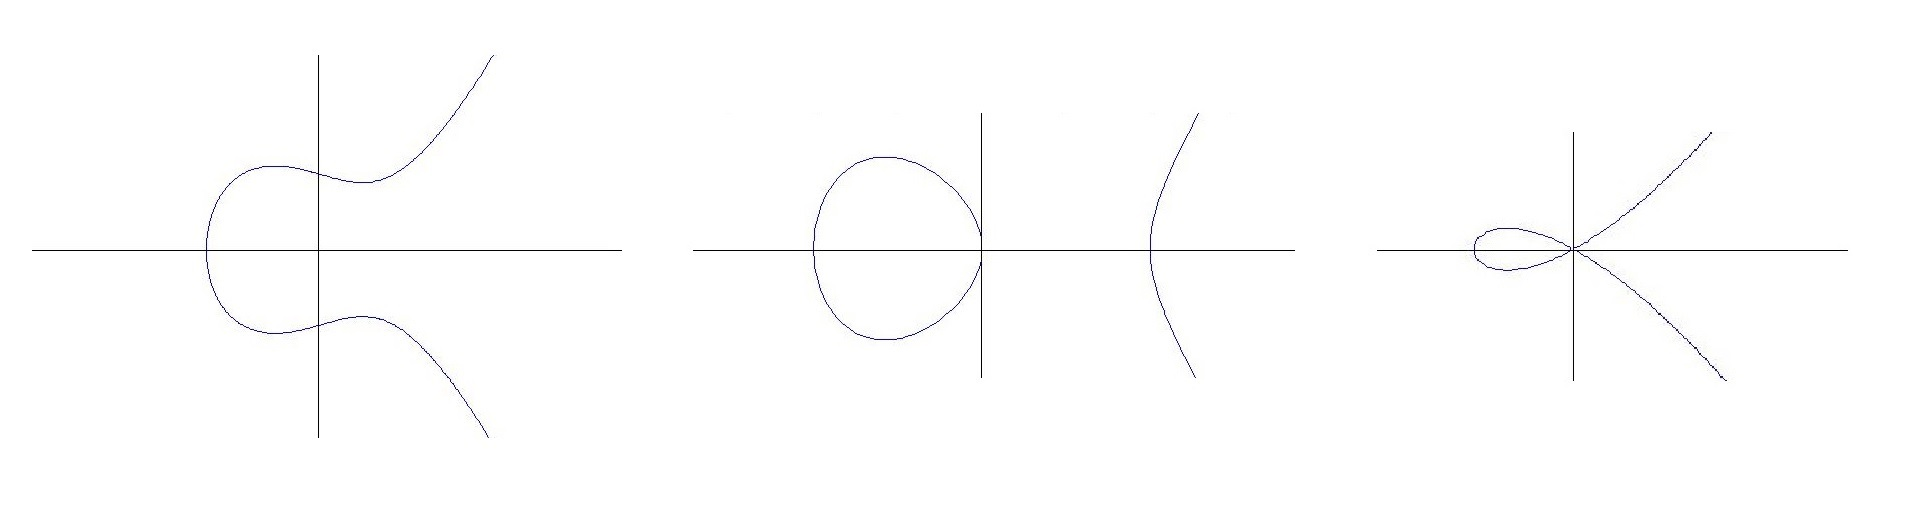
\includegraphics[width=15cm, height=5cm]{ellcurvesexamples}
\begin{center} Figure 1: The zero loci of three (not all nonsingular) Weierstrass equations. \end{center}

As usual a curve $C$ given by a Weierstrass equation is \emph{defined over $K$} if $a_1,\ldots,a_6 \in K$. To simplify notation, the Weierstrass equation will generally be given using non-homogeneous coordinates $x:=X/Z$ and $y:=Y/Z$, \begin{equation}\label{generalweierstrassequation}C:y^2+a_1xy+a_3y=x^3+a_2x^2+a_4x+a_6.\end{equation} Thus the curve $C$ has an affine open part given by this equation and a unique point $O:=[0,1,0]$ at infinity. This point is called the \emph{base point} of $C$. If $C$ is defined over $K$, then the set of $K$-rational points is the following: $$C(K):=\{(x,y)\in K^2\; | \; y^2+a_1xy+a_3y=x^3+a_2x^2+a_4x+a_6\}\cup \{O\}.$$ 

\begin{remark}\label{weierstrassmeanselliptic}
A consequence of \emph{Hurwitz theorem} \cite[II.5.9.]{Silverman} is that curves $C$ in $\proj{2}$ given by a nonsingular homogeneous polynomial of degree $d \ge 1$ have genus $$\text{genus}(C)=\frac{(d-1)(d-2)}{2}.$$ It thus follows that any curve $C$ given by a Weierstrass equation has $\text{genus}(C)=1$. Hence this curve together with the base point $O=[0,1,0]$ is an elliptic curve.
\end{remark}

Associated to an elliptic curve the following quantities are defined:
\begin{equation}\label{quantitiesellcurve}
\begin{align*}
b_2 &= a_1^2 +4a_4 \\
b_4 &= 2a_4+a_1a_3 \\
b_6 &= a_3^2+4a_6 \\
b_8 &= a_1^2a_6+4a_2a_6-a_1a_3a_4+a_2a_3^2-a_4^2 \\
c_4 &= b_2^2-24b_4 \\
c_6 &= -b_2^3+36b_2b_4-216b_6 \\
\Delta &= -b_2^2b_8 -8b_4^3-27b_6^2+9b_2b_4b_6 \\
j &= c_4^3/\Delta \\
\omega &= \frac{dx}{2y+a_1x+a_3} = \frac{dy}{3x^2+2a_2x+a_4-a_1y}
\end{align*}
\end{equation}

\begin{definition}\label{disc.omega.and.j}
The quantity $\Delta$ is called the \emph{discriminant} of the Weierstrass equation, $j$ is called the \emph{$j$-invariant} of the elliptic curve and the differential $\omega$ is called the \emph{invariant differential} associated to the Weierstrass equation.
\end{definition}

The reason that $\omega$ is called the invariant differential is that it is \emph{translation invariant}. I will now specify what this means.  

\begin{definition}\label{translationmap}
Let $E$ be an elliptic curve and $Q \in E$ a point of $E$. The \emph{translation-by-Q map} $\tau_Q$ is the map $$\tau_Q:E \rightarrow E, \qquad P \mapsto P+Q.$$
\end{definition}

This map is a morphism of curves by proposition \ref{multismorphism}. Recall that $\omega$ is a differential form on an elliptic curve. For the sake of notation, I will give the definition here.

\begin{definition}\label{diffdef}
Let $C$ be a curve. The space of differential forms on $C$, denoted by $\Omega_C$, is the $\bar{K}$-vector space generated by symbols of the form $dx$ for $x \in \bar{K}(C)$, subject to the relations:
\begin{itemize}
\item $d(x+y)=dx+dy$ for all $x,y\in\bar{K}(C)$.
\item $d(xy)=xdy+ydx$ for all $x,y \in \bar{K}(C)$. 
\item $d\lambda = 0$ for all $\lambda \in \bar{K}$.
\end{itemize}
\end{definition}

This space $\Omega_C$ turns out to ba a 1-dimensional $\bar{K}(C)$-vector space, as is proven in \cite[II.4.2]{Silverman}.
Remark that any non constant morphism of curves $\phi:C_1 \rightarrow C_2$ induces a map on function fields $\phi^*: \bar{K}(C_2) \rightarrow \bar{K}(C_1)$ which in turn induces a map on differential forms $\phi^*: \Omega_{C_2} \rightarrow \Omega_{C_1}$.

\begin{proposition}\label{translationinvariance}
Let $E$ be an elliptic curve given by a Weierstrass equation, $Q\in E$ be any point of $E$ and let $\tau_Q$ denote the translation-by-$Q$ map. Then the invariant differential $\omega$ satisfies $$\tau_Q^* \omega = \omega.$$
\end{proposition}

This property is referred to as the `translation invariance' of $\omega$. The importance of the discriminant and the $j$-invariant are given by the following proposition.

\begin{proposition}\label{disc&jinv}
\begin{enumerate}
\item A (not necessarily nonsingular) Weierstrass equation is nonsingular if and only if $\Delta \neq 0$.
\item Two curves given by nonsingular Weierstrass equations are isomorphic over $\bar{K}$ if and only if they share the same $j$-invariants.
\end{enumerate}
\end{proposition}

The enormous use of Weierstrass equations is the fact that any elliptic curve is isomorphic to a curve given by a Weierstrass equation. This fact is made precise in the following theorem. Because this theorem is such a beautiful application of the Rieman-Roch theorem, I will give a summary of the proof here.

\begin{proposition}
Let $(E,O)$ be an elliptic curve defined over $K$. There exist functions $x,y \in K(E)$ such that the map $$\phi:E \rightarrow \proj{2},\quad \phi=[x,y,1]$$ gives an isomorphism of $E/K$ to a curve given by a nonsingular Weierstrass equation (\ref{weierstrassequation}) with coefficients $a_1,\ldots,a_6 \in K$ and such that $\phi(O)=[0,1,0]$. The functions $x$ and $y$ are called the Weierstrass coordinates for the elliptic curve $E$.
\end{proposition}

\begin{proof}
Let $E/K$ be an elliptic curve defined over a field $K$ and let $n \geq 1$ be a positive integer. Then the Riemann-Roch theorem implies that, since $E$ has genus $1$, the vector space $\mathcal{L}(n(O))$ has dimension $$\ell\big(n(O)\big)=\text{dim}_{\bar{K}}\mathcal{L}\big(n(O)\big)=n.$$ It is thus possible to choose functions $x,y \in K(E)$ such that $\{1,x\}$ is a basis for $\mathcal{L}\big(2(O)\big)$ and $\{1,x,y\}$ is a basis for $\mathcal{L}\big(3(O)\big)$. Note that $x$ has a pole of exact order $2$ at $O$ and $y$ has a pole of exact order $3$ at $O$. Now it is clear that $\mathcal{L}\big(6(O)\big)$, which has dimension $6$, contains the following seven functions: $$1,x,y,x^2,xy,y^2,x^3.$$ Thus there is a linear relation $A_1+A_2x+A_3y+A_4x^2+A_5xy+A_6y^2+A_7x^3=0$. It turns out that $A_1,\ldots,A_7 \in K$ and $A_6A_7 \neq 0$. (This will not be proven here.) This last fact allows a substitution for $x$ and $y$ such that the image of the map $\phi=[x,y,1]$ actually lies in the zero locus of a Weierstrass equation. Also $\phi(O)=[0,1,0]$, since $y$ has a higher-order pole at $O$ than $x$. Now it only remains to show that the map $\phi$ is an isomorphism and that the found Weierstrass equation is actually nonsingular. The proposition then follows. 
\end{proof}


In certain instances the Weierstrass equation can actually be simplified. For example, if $\Char{\bar{K}}\neq 2$, then, using some substitution for $y$, the equation can be simplified to $$y^2=4x^3+b_2x^2+2b_4x+b_6.$$ If $\Char{\bar{K}}\neq 2,3$ then further substitution can be used to eliminate the $x^2$ term in this equation, yielding an equation of the form \begin{equation}\label{weierstrasshighchar}y^2=x^3+Ax+B,\end{equation} where $A=-27c_4$ and $B = -54c_6$. Recall that the quantities $b_i$ and $c_i$ were given this section in \ref{quantitiesellcurve}. Associated to this last equation the discriminant and $j$-invariant become the following quantities: $$\Delta=-16(4A^3+27B^2) \quad j=-1728\frac{(4A)^3}{\Delta}.$$




\subsection{The Geometric Group Law}\label{geometricgrlaw} 
In this section $E$ will be an elliptic curve given by a Weierstrass equation $$E:y^2+a_1xy+a_3y=x^3+a_2x^2+a_4x+a_6.$$ I will give the group law on $E$ explicitly. To do this, let $L \subseteq \proj{2}$ be a line. Then B\'ezout's theorem \cite[I.7.8.]{Hartshorne} implies that $L\cup E$ consists of exactly three points. (Counted with multiplicities.) This fact will now be used to define a composition law $\oplus$ on $E$:

\begin{compositionlaw} \label{composition}
Let $P,Q$ be two (not necessary distinct) points on $E$ and let $L$ be the line through $P$ and $Q$. (Remark that if $P=Q$, then $L$ is the tangent line to $E$ at $P$.) Let then $R$ be the third point of intersection of $L$ with $E$. Now let $L'$ be the line through $R$ and $O$ (the base point of $E$). Then $P\oplus Q$ is defined to be the third point of intersection of $L'$ with $E$.
\end{compositionlaw}

One instance of the composition law is illustrated in Figure 2. It turns out that this composition law $\oplus$ actually is the algebraic group law on $E$ given in definition \ref{grplawgeneral}.

\begin{proposition}\label{grplawsaresame}
Let $E$ be an elliptic curve and $P,Q\in E$ be two points on $E$. Then $$P \oplus Q = P+Q.$$ 
\end{proposition}

\begin{proof}
Remark that by the definition of $P+Q=\sigma\big(\nu(P)+\nu(Q)\big)$ (\ref{grplawgeneral}), it suffices to show that $$\nu(P\oplus Q) = \nu(P)+\nu(Q).$$ Let now $L$, $L'$ and $R$ be as in the composition law, where $L$ and $L'$ are the zero locus of the functions $f$, $f'$ respectively. So explicitly: \begin{align*}
L:\alpha X+\beta Y + \gamma Z &=f(X,Y,Z)=0,\\
L': \alpha' X + \beta' Y + \gamma' Z &= f'(X,Y,Z)=0.
\end{align*} 

\begin{center}
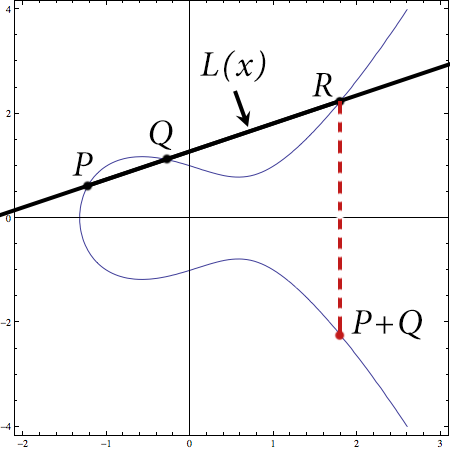
\includegraphics[scale=.25]{addpointsexample}\\
Figure 2: The composition law.
\end{center}

Then from the definition of the composition law and the fact that the line $Z=0$ intersects $E$ at $O$ with multiplicity $3$ the following is clear: \begin{align*}
\text{div}(f/Z) &= (P)+(Q)+(R)-3(O),\\
\text{div}(f'/Z) &= (R)+(P\oplus Q) -2(O).
\end{align*}
And thus $0 \sim \text{div}(f'/f)=(P \oplus Q) - (P)-(Q)+(O)$, which means that $$\nu(P \oplus Q) - \nu(P)-\nu(Q) = 0.$$
\end{proof}

Since the composition law $\oplus$ is just the algebraic group law of $E$, it will from now on simply be denoted by `+'. Remark that in the composition law it is vital that $E$ is assumed to be nonsingular ($\Delta \neq 0$). In fact if $P$ were a singular point of $E$, then the tangent space to $E$ at $P$ would be $2$-dimensional, thus not a line at all. Obviously the composition law used to define the point $P + P$ would make no sense. However if the Weierstrass equations were singular, then the nonsingular points of its zero locus would still form an abelian group.

\begin{definition}\label{Enspart}
Let $E$ be the zero locus of a (possibly singular) Weierstrass equation. The set of nonsingular points of $E$ is denoted $\Enonsing$ and usually called the \emph{nonsingular part of $E$}. If $E$ is defined over $K$, then $\Enonsing(K)$ is the set of nonsingular points of $E(K)$.
\end{definition}

\begin{proposition}
Let $E$ be the zero locus of a singular Weierstrass equation. Then the composition law \ref{composition} on $\Enonsing$ turns it into an abelian group.
\end{proposition}

Since the main focus of this paper will be on the ECDLP, the following definition will not come as a suprise.

\begin{definition}\label{multmap}
Let $P\in E$ and $m \in \ZZ$, then $[m]P$ is defined as follows:
$$[m]P:=\underbrace{P+\ldots+P}_{\text{m times if } m>0},\qquad
[m]P&:=\underbrace{-P-\ldots-P}_{\text{-m times if } m<0},\qquad
[0]P&:=O$$
\end{definition}

In order to work with elliptic curves as a group it is necessary to have an algorithm which produces for two points $P_1,P_2\in E$ the point $P_3:=P_1+P_2$. This algorithm is easy to extract from the composition law and will just be stated here without proof. One important fact to note is that for a point $P_0=(x_0,y_0) \in E$ the point $-P_0$ equals $$-P_0=(x_0,-y_0-a_1x_0-a_3).$$ \newpage

\begin{algorithm}\label{grplawalg}
\caption{Elliptic Curve Group law}
\begin{algorithmic}[1]
  \normalsize
  \REQUIRE An elliptic curve $E$, two point $P_i=[x_i,y_i,1]\in E$ where $i \in \{1,2\}$.
  \ENSURE The point $P_3=P_1+P_2$.
  \IF{$x_1=x_2$ and $y_1+y_2+a_1x_2+a_3=0$}
  \STATE{$P_3 \leftarrow O$}
  \ELSE
  \IF{$x_1 = x_2$}
  \STATE{$\lambda \leftarrow$ {\Large$\frac{3x_1^2+2a_2x_1+a_4-a_1y_1}{2y_1+a_1x_1+a_3}$}, \quad $\nu \leftarrow$ {\Large$\frac{-x_1^3+a_4x_1+2a_6-a_3y_1}{2y_1+a_1x_1+a_3}$}}
  \ELSE
  \STATE{$\lambda \leftarrow$ {\Large$\frac{y_2-y_1}{x_2-x_1}$},\quad $\nu \leftarrow$ {\Large$\frac{y_1x_2-y_2x_1}{x_2-x_1}$}}
  \ENDIF
  \STATE{$x_3 \leftarrow \lambda^2+a_1\lambda-a_2-x_1-x_2$, \quad $y_3 \leftarrow -(\lambda+a_1)x_3-\nu-a_3$}
  \STATE{$P_3 \leftarrow [x_3,y_3,1]$}
  \ENDIF 
  \RETURN{$P_3$}
\end{algorithmic}
\end{algorithm}

If we want to calculate $[m]P$ for rather large $m$, the binary representation of $m$ can be used to calculate $[m]P$ more efficiently:

\begin{algorithm}\label{binaryptmult}
\caption{Point multiplication: Binary Method}
\begin{algorithmic}[1]
  \normalsize
  \REQUIRE A point $P \in E$ and an integer $m=\sum_{j=0}^k m_j2^j$, $m_j \in \{0,1\}$.
  \ENSURE The point $Q=[m]P$.
  \STATE{$Q \leftarrow O$}
  \FOR{$j = k$ to $0$ by $-1$}
  \STATE{$Q \leftarrow [2]Q$}
  \IF{$k_j=1$}
  \STATE{$Q \leftarrow Q+P$}
  \ENDIF
  \ENDFOR
  \RETURN{$Q$}
\end{algorithmic}
\end{algorithm}

This algorithm requires order $O(\log m)$ point additions in $E$. Another way to calculate $[m]P$ efficiently is using \emph{division polynomials}. More information on this will be given in section \ref{divpolsection}.
Remark that if an elliptic curve $E$ is given over a field $K$ of $\Char{K} \neq 2,3$, it can be given by an  equation like \ref{weierstrasshighchar}, and then for a point $P_0=(x_0,y_0) \in E$ we actually have \begin{equation}\label{minushighchar}-P_0=(x_0,-y_0).\end{equation} I will conclude this section with a short example:

\begin{example}\label{fingrpex}
Let $p=13$ and let $E/\FF{p}$ be given by the Weierstrass equation $E:y^2=x^3+2$. Then $E$ has discriminant $\Delta=-1728 \not \equiv 0$ (mod 13) and is thus nonsingular. In \ref{ptcountingLS} a method will be given to compute the number of rational points $\#E(\FF{p})$. It turns out that $\#E(\FF{p})=19$, thus, since 19 is a prime number, this group is cyclic. However the group $E(\FF{p^2})$ has $171=3^2*19$ elements. Let $C_n$ denote the cyclic group of order $n$ for any positive integer $n$. A basic group theoretical result  (given in \ref{fingrpstructure}) implies that either $E(\FF{p^2}) \cong C_{171}$ or $E(\FF{p^2}) \cong   C_{57} \times C_3$ and we would like to determine which of these two cases is true. All points $P=(x_0,y_0) \in E(\FF{p^2})$ can be computed by checking for all $x_0 \in \FF{p^2}$ whether $x_0^3+2$ is a square in $\FF{p^2}$ and, if it is, determining the roots. If this is done, then $[3]P$ and $[57]P$ can be computed for all points $P\in E(\FF{p^2})$. It turns out that for all points $P$ either $[3]P = O$ or $[57]P=O$. Thus $E(\FF{p^2})$ cannot be cyclic of order $171$, thus it is isomorphic to $C_{57} \times C_3$. In fact for all curves defined over a finite field $\FF{q}$, the group $E(\FF{q})$ will turn out to be generated by $\leq 2$ elements. This will be proven in \ref{finiteECstruc}. Also in section \ref{reduction} an algorithm will be given to determine the group structure of an elliptic curve over a finite field.
\end{example}




\subsection{Isogenies}\label{isogenies}
Until now some of the basic properties of elliptic curves have been examined. A natural next step is to study maps between two such curves. Since elliptic curves are both algebraic varieties and abelian groups, it will not come as a surprise that these maps are assumed to respect both of these structures. The following definition can be given more generally for group varieties, but since these objects are not assumed to be part of the required background knowledge, I will just give the definition for maps of elliptic curves.

\begin{definition}
Let $(E_1,O_1)$, $(E_2,O_2)$ be elliptic curves. A \emph{homomorphism of elliptic curves}  is a morphism $f:E_1 \rightarrow E_2$ of algebraic varieties , such that $f$ is also a homomorphism of abelian groups. Such a homomorphism $f:E_1 \rightarrow E_2$ is called an \emph{isogeny} if it is finite and surjective.
\end{definition}

In fact, in order for a morphism of algebraic varieties to be a homomorphism of elliptic curves, it suffices to check whether it respects base points, as the following theorem states:

\begin{theorem}
Let $(E_1,O_1)$, $(E_2,O_2)$ be elliptic curves and let $f:E_1 \rightarrow E_2$ be a morphism of algebraic varieties such that $f(O_1)=O_2$. Then $$f(P+Q)=f(P)+f(Q) \qquad \text{for all } P,Q \in E_1.$$
\end{theorem}

The following lemma from \cite[II.6.8]{Hartshorne} follows from the basic properties of algebraic curves. 

\begin{lemma}\label{isobasicproperty}
Let $f:E_1 \rightarrow E_2$ be a homomorphism of elliptic curves curves, then $f$ is an isogeny if and only if $f \neq [0]$. 
\end{lemma}

Two elliptic curves are called \emph{isogenous} if there exists an isogeny between them. This will turn out to be an equivalence relation, as will be shown in \ref{isoequivalence}.

\begin{example}\label{multbymmap}
Let $E$ be an elliptic curve and let $m \in \mathbb{Z}$, then the multiplication-by-$m$ map $[m]:E \rightarrow E$ as defined in \ref{multmap} is an endomorphism of $E$. If furthermore $m \neq 0$, then $[m]$ is actually an isogeny. (This is a direct consequence of proposition \ref{multbymmapproperties}.)
\end{example}

\begin{definition}
Let $f: C_1 \rightarrow C_2$ be a morphism of algebraic curves, it induces an injection of function fields $$f^*: \bar{K}(C_2) \rightarrow \bar{K}(C_1).$$ The \emph{degree} of $f$, which is denoted by $\degree{f}$, is the degree of the finite field extension $\bar{K}(C_1) / f^* \bar{K}(C_2).$ The separable and inseparable degrees of $f$ are defined accordingly and are denoted by $\sdegree{f}$ and $\idegree{f}$ respectively. Also the morphism is called separable, inseparable or purely inseparable according to the corresponding property of the field extension. By convention the zero homomorphism $[0]$  is said to have $\degree{[0]}=0.$
\end{definition}

Of course this definition extends to homomorphisms of elliptic curves. Recall that for a non constant morphism of curves $f:C_1 \rightarrow C_2$ and a point $P \in C_1$, the \emph{ramification index} of $f$ at $P$ can be defined. In this thesis the ramification index of $f$ at $P$ is denoted by $e_f(P)$. For the definition and the basic properties of this notion I refer to \cite[II.2]{Silverman}. The following theorem gives some important results relating the (in)separable degrees of a morphism. This theorem is a basic result for morphisms of algebraic curves and is only stated here as a reminder to the reader. 

\begin{theorem}\label{degreetheorem}
Let $f: C_1 \rightarrow C_2$ be a non constant morphism of algebraic curves, then for every $Q \in C_2$, $$\#\{P \in C_1 \; | \; f(P)=Q\}=\sdegree{f}.$$ Furthermore for every $P \in C_1$, $$e_f(P)=\idegree{f}.$$
\end{theorem}

A consequence of this theorem is that, if $f$ is separable, then for each $Q \in C_2$, $$\#\{P \in C_1 \; | \; f(P)=Q\} = \sdegree{f} = \degree{f}.$$ Hence $f$ is unramified and \begin{equation}\label{kernelisdegree}\#\kernel{f} = \degree{f}.\end{equation} The following proposition provided a useful criterion for determining whether a morphism of curves is actually separable.

\begin{proposition}\label{separablecrit}
Let $f:C_1 \rightarrow C_2$ be a non constant morphism of curves. Then $f$ is separable if and only if the induced map on differential forms $$f^*:\Omega_{C_2} \rightarrow \Omega_{C_1}$$ is injective. (Remark that, since $\Omega_{C_i}$ are $1$-dimensional $\bar{K}(C_i)$-vector spaces for $i=1,2$, this condition is equivalent to the condition that $f^*$ is nonzero.)
\end{proposition}

Another nice property of the degree-map is that for two subsequent morphisms $C_1 \overset{f}{\rightarrow} C_2 \overset{g}{\rightarrow} C_3$ the following holds: \begin{equation}\label{degreeconcatenation}\degree{g \circ f}=\degree{g} \cdot \degree{f}.\end{equation}

\begin{definition}
Let $E,E_1,E_2$ be elliptic curves, then the group of homomorphism from $E_1$ to $E_2$ is denoted by $$\text{Hom}(E_1,E_2),$$ where the group operation is defined by $(f+g) (P) = f(P) + g(P)$. Remark that the identity element of this group is the zero homomorphism $[0]$. The group of endomorphism from $E$ to $E$ is denoted by $$\Endring{E} = \text{Hom}(E,E).$$ This turns out to be a ring whose addition law is given by the addition law of $\text{Hom}(E,E)$ and whose multiplication is composition of endomorphisms. $(g\cdot f)(P)=g(f(P))$ This ring is called the \emph{endomorphism ring} of $E$. The invertible elements of this ring form the \emph{automorphism group} of $E$ which is denoted by $\Autgrp{E}.$ If the elliptic curves are defined over a field $K$, the subgroup (or ring) of homomorphism defined over $K$ are denoted by $$\text{Hom}_K(E_1,E_2),\quad \Endringk{E}{K},\quad \Autgrpk{E}{K}.$$ 
\end{definition}

The following proposition gives two important properties of the multiplication-by-$m$ map:

\begin{proposition}\label{multbymmapproperties} Let $E$ be an elliptic curve defined over $K$ and $m \in \ZZ$, then the multiplication-by-$m$ map $[m]$ satisfies $$[m] \in \Endringk{E}{K}.$$ If furthermore $m \neq 0$, then the map $[m]$ is non constant.
\end{proposition}

From this proposition it is clear that the endomorphism ring $\Endring{E}$ has characteristic $0$. Also it is easy to see that it has no zero divisors (ie. it is an integral domain), for suppose that $f$, $g \in \Endring{E}$ satisfy $g \circ f =[0]$, then $$\degree{g}\degree{f}=\degree{g \circ f} = 0.$$ This implies that either $f = [0]$ or $g = [0]$.\par 
The following definition will play a very important role in this paper:

\begin{definition}\label{mtorsionpoints}
Let $E$ be an elliptic curve and $m$ be a positive integer. The subgroup of $m$-torsion points of $E$ is denoted $$E[m]=\{P \in E \; | \; [m]P=O\}$$ and called the \emph{$m$-torsion subgroup} of $E$. The \emph{torsion subgroup} of $E$ is denoted by $E_\text{tors}$. This is the group defined by $E_\text{tors} = \bigcup_{m=1}^\infty E[m]$. If $E$ is defined over $K$, then $E_\text{tors}(K)$ denotes the points of finite order in $E(K)$. Similarly $E(K)[m]$ will denote the points of order $m$ in $E(K)$.
\end{definition}

\begin{example}
As in example \ref{fingrpex} let $E/\FF{13}$ be given by $y^2=x^3+2$. Then $E(\FF{13})$ was seen to be cyclic of order $19$. A direct consequence is that $$E(\FF{13})[19] \cong C_{19}$$ (the cyclic group of order $19$). In fact for all $i \neq 0$ we have $E(\FF{13})[19i] \cong C_{19}$ and $E(\FF{13})[m] = \{O\}$ for all other $m \in \ZZ$. Also it was stated that $E(\FF{13^2}) \cong   C_{57} \oplus C_3$. Note that $57=3*19$. Now it is an easy exercise to show that $$E(\FF{13^2})[3] \cong C_3 \oplus C_3 \quad \text{and} \quad E(\FF{13^2})[19] \cong C_{19}. $$ Also $E(\FF{13^2})[m] =\{O\}$ for all integers $m$ such that $\gcd(m,57)=1$, since $E(\FF{13^2})$ has only points of exact order $1,3,19$ or $57$. let now $i$ be a nonzero integer such that $\gcd(i,19)=1$. Then the only points $P\in E(\FF{13^2})$ which satisfy $[3i]P=O$ are the points of exact order $3$, since either the order of such a point $P$ is a multiple of three or, if this is not the case, the order divides $i$. So $$E(\FF{13^2})[3i]\cong C_3 \oplus C_3.$$  Similarly it is clear that for all nonzero $j$ such that $\gcd(j,3)=1$ the following holds $$ E(\FF{13^2})[19j]\cong C_{19}. $$ The only torsion groups of $E(\FF{13^2})$ left are the torsion groups $E(\FF{13^2})[57k]$ for some nonzero integer $k$. However all points $P$ of $E(\FF{13^2})$ satisfy $[57]P=O$, thus we simply have $$E(\FF{13^2})[57k] \cong C_3 \oplus C_{57}.$$
\end{example}

If we assume $E/K$ is an elliptic curve, then the homomorphism $$[\;]:\ZZ \rightarrow \Endring{E}$$ is always injective by \ref{multbymmapproperties}. It is very well possible that this map is actually a ring isomorphism. If this is not the case however, then $E$ is said to have \emph{complex multiplication}, or CM for short. In theorem \ref{FFEndring} will be shown that if $K$ is a finite field, then $\Endringk{E}{K}$ will always have complex multiplication.

\begin{example} \label{morphism[i]}
Suppose $\Char{K} \neq 2$ and let $i\in\bar{K}$ be a fourth root of unity. Thus $i^2 = -1$. Furthermore let $E/K$ be the elliptic curve given by $$E:y^2=x^3+x.$$ Then it is not so hard to see that the map $$[i]:(x,y) \mapsto (-x,iy)$$ is an isogeny from $E$ to itself. It is however not a multiplication-by-$m$ map. This follows from the fact that $[i]\circ [i] = [-1]$ thus if $[i]=[m]$ for some integer $m\in \ZZ$, then $[-1] = [m] \circ [m] = [m^2]$ and this is impossible. Thus $E$ has complex multiplication. Also clearly the isogeny $[i]$ is defined over $K$ if and only if $i \in K$. This example thus shows that even if $E$ is defined over $K$, it is possible that $\Endringk{E}{K}$ is strictly smaller than $\Endring{E}$.
\end{example}




\subsection{The Frobenius Morphism}\label{frobenius}
It is hard to overestimate the importance of the \emph{Frobenius morphism} when studying elliptic curves over finite fields. In this section the Frobenius morphism will be defined and some of its basic properties will be given.\par  
For the rest of this section it will be assumed that $p$ is a prime and $q=p^r$ for some positive integer $r$. Assume that $\Char{K}=p$. For any polynomial $f \in K[X]$ let $f^{(q)}$ be the polynomial obtained from $f$ by raising each coefficient to the $q^{\text{th}}$ power. If now $C/K$ is any curve, then $C^{(q)}/K$ is the curve whose homogeneous ideal is given by $$I(C^{(q)}):= \grgen{f^{(q)} \; | \; f \in I(C)}.$$
The $q^{\text{th}}$ Frobenius morphism is the morphism $\frob :C \rightarrow C^{(q)}$ given by 
\begin{equation}\label{frobdefinition}\frob :[x_0,\ldots,x_n] \mapsto [x_0^q,\ldots,x_n^q].\end{equation} To see that $\frob$ actually maps $C$ into $C^{(q)}$, take any point $P:=[x_0,\ldots,x_n] \in C$ and an element $f$ of $I(C)$. Then the following calculation suffices:
\begin{align*}
f^{(q)}(\frob(P)) &=f^{(q)}(x_0^q,\ldots,x_n^q) \\
&=(f(x_0,\ldots,x_n))^q &\text{since } \Char{K}=p,\\
&=0 &\text{since }f(P)=0.
\end{align*}

Remark that the Frobenius morphism is only defined if the field $K$ has characteristic $p$. The following two propositions give some basic, but important, properties of the Frobenius morphism:

\begin{proposition}\label{frobproperties}
Let $C/K$ be a curve with $\Char{K} = p$ and let $\frob:C \rightarrow C^{(q)}$ be the $q^\text{th}$ Frobenius morphism, then
\begin{itemize}
\item $\frob$ is purely inseparable,
\item its degree equals $\degree{\frob} = q$.
\end{itemize}
\end{proposition}

\begin{proposition}\label{frobfactorization}
Let $\psi:C_1 \rightarrow C_2$ be a morphism of curves defined over a field of characteristic $p>0$. Then $\psi$ factors as $$C_1 \overset{\frob}{\longrightarrow} C_1^{(q)} \overset{\lambda}{\longrightarrow} C_2, $$ where $q=\idegree{\psi}$, the morphism $\lambda$ is separable and $\frob$ denotes the $q^\text{th}$ Frobenius morphism.
\end{proposition}

\begin{example}\label{1-frobenius}
Let $K:=\FF{q}$ and $C/K$ be a curve defined over the finite field $\FF{q}$. It is a well known fact that $x \in \FFCL{q}$ satisfies $x^q = x$ if and only if $x \in \FF{q}$. \cite[App. C]{Waterhouse} This fact has two very important consequences:
\begin{enumerate}
\item Since the ideal $I(C)$ can be generated by some polynomials $(f_i)_{i \leq n}$ with coefficients in $\FF_q$ (which means that $f_i^{(q)}=f_i$), it is clear that $C^{(q)}=C$.
\item If $P=[x_0,\ldots,x_n] \in C$, then $\frob(P)=P$ if and only if $x_i \in \FF{q}$ for all $0 \leq i \leq n$. This means that $C(\FF{q})=\kernel{[1]-\frob}$.
\end{enumerate}
\end{example}

From now on the map $[1]-\frob$ will simply be denoted by $1-\frob$. If $C$ is an elliptic curve (called $E$), then the map $1-\frob$ is an endomorphism of $E$ and $$\#E(\FF{q})=\degree{1-\frob}.$$ This statement follows from theorem \ref{degreetheorem} and the fact that $1-\frob$ is separable. The rest of this section will be devoted to the deduction of the separability of $1-\frob$.

\begin{proposition}
Let $E_1$ and $E_2$ be elliptic curves given by Weierstrass equations and let $\omega$ be the invariant differential on $E_2$. If furthermore $f,g: E_1 \rightarrow E_2$ are two isogenies, then $$(f+g)^*\omega=f^* \omega + g^* \omega.$$
\end{proposition}

For this proposition the translation invariance of the invariant differential (\ref{translationinvariance}) is crucial. With induction on $m$ the following follows naturally from this proposition.

\begin{corollary}\label{invdiffislinear}
Let $E$ be an elliptic curve given by a Weierstrass equation and let $\omega$ be the invariant differential associated to the Weierstrass equation. Let also $m\in \ZZ$. Then the following equality holds: $$[m]^* \omega = m \omega.$$
\end{corollary}

With help of this result it is now possible to proof that the map $1-\frob$ is separable. Actually, a stronger result will be proven:

\begin{corollary}\label{frobseparable}
Let $E/\FF{q}$ be an elliptic curve given by a Weierstrass equation. (Recall that $q$ was assumed to be a prime power $p^r$.) Let furthermore $\frob:E \rightarrow E$ be the $q^{\text{th}}$ Frobenius morphism and $m,n \in \ZZ$. Then the map $$m+n\frob:E \rightarrow E$$ is separable if and only if $p \nmid m$.
\end{corollary}

\begin{proof}
Let $\omega$ be the invariant differential. From \ref{separablecrit} it follows that a morphism $\phi: E \rightarrow E$ is inseparable if and only if $\phi^* \omega = 0$. Thus, since $\frob$ is inseparable, (\ref{frobproperties}) $\frob^*\omega = 0$ which means that: $$(m+n\frob)^*\omega=[m]^* \omega + ([n]^* \circ \frob^*) \omega = m\omega.$$ And the desired result follows from the remark that $m\omega = 0$ if and only if $p \mid m$.
\end{proof}






\subsection{The Dual Isogeny}
If $E$ is an elliptic curve and $m\in\ZZ$ a positive integer, then the $m$-torsion subgroup $E[m]$ has a very specific structure. In order to find this structure it is useful to develop the notion of the \emph{dual isogeny} to a given isogeny $f$. It is possible to concretely construct this dual isogeny if $f$ is given. However that will not be done here. I will be content with formulating the definition and stating its most important properties. 

\begin{proposition}\label{dualisoproperty}
Let $f: E_1 \rightarrow E_2$ be a non constant isogeny of elliptic curves of degree $m$.  Then there exists a unique isogeny $\hat{f}: E_2 \rightarrow E_1$ such that $$\hat{f} \circ f = [m]$$
\end{proposition}

\begin{definition}\label{dualisogeny}
Let $f: E_1 \rightarrow E_2$ be an isogeny of elliptic curves. Then the dual isogeny to $f$ is the isogeny $\hat{f}$ given in \ref{dualisoproperty}.
\end{definition}

\begin{remark}\label{isoequivalence}
Two elliptic curves were called isogenous if there exists an isogeny between them. It is clear that \emph{being isogenous} is a reflexive and transitive relation on elliptic curves by considering the isogeny $[1]$ and composition of isogenies respectively. Proposition \ref{dualisoproperty} now ensures that this relation is also symmetric. Thus being isogenous is actually an equivalence relation on elliptic curves.
\end{remark}


\begin{example}
Just as in example \ref{morphism[i]} let $\Char{K}\neq 2$ and let $E/K$ be given by $E:y^2=x^3+x$. Furthermore let $i\in\bar{K}$ be a primitive fourth root of unity and let $$[i]:E \rightarrow E \quad \text{be defined by} \quad [i]: (x,y) \mapsto (-x,iy).$$ As we have seen, $[i]^2=[-1]$, which means that $[i]^4=[1]$. Hence we are dealing with an isomorphism with inverse $[i]^{-1}=[i]^3$. This implies that $\degree{[i]}=1$. The dual isogeny to $[i]$ is thus given by $$\widehat{[i]}=[i]^3:(x,y) \mapsto (-x,-iy).$$ 
\end{example}

The following theorem states the most important properties of the dual isogeny. 

\begin{theorem}\label{dualisoproperties}
Let $f: E_1 \rightarrow E_2$ be an isogeny of elliptic curves and let $\hat{f}:E_2 \rightarrow E_1$ be its dual.
\begin{enumerate}
\item Let $m=\degree{f}$. Then $\hat{f} \circ f =[m]$ on $E_1$ and $f \circ \hat{f} = [m]$ on $E_2$.
\item Let $g: E_2 \rightarrow E_3$ be another isogeny. Then $\widehat{g \circ f}=\hat{f} \circ \hat{g}.$
\item Let $h: E_1 \rightarrow E_2$ be another isogeny. Then $\widehat{f+h} = \hat{f} + \hat{h}$.
\item Suppose $m\in \ZZ$, then $\widehat{[m]}=[m]$ and $\degree{[m]}=m^2$.
\item $\deg (\hat{f})=\degree{f}$.
\item $\hat{\hat{f}}=f$.
\end{enumerate}
\end{theorem}

The fact that $\degree{[m]}=m^2$ is very important. It induces the following beautiful result:

\begin{corollary}\label{torgrpstructure}
Let $E/K$ be an elliptic curve and $0 \neq m \in \ZZ$.
\begin{itemize}
\item If either $\Char{K}=0$ or $\Char{K}=p>0$ and $p \nmid m$, then $$E[m]\cong\Zmod{m}\times \Zmod{m}.$$
\item If $\Char{K}=p>0$, then one of the following is true:
\begin{itemize}
\item $E[p^r]=\{O\} \quad \quad$ for all $r=1,2,\ldots$.
\item $E[p^r]\cong\Zmod{p^r} \quad$ for all $r=1,2,\ldots$.
\end{itemize}
\end{itemize}
\end{corollary}

The only case in which the group structure of the $[m]$-torsion points of $E$ is not yet known, is when char$(K)=p>0$ such that $p \mid m$ but $m$ is not a power of $p$. However in this case corollary \ref{torgrpstructure} can still be used to determine the group structure of $E[m]$:

\begin{lemma} \label{torgrpremark}
Let $E/K$ be an elliptic curve with char$(K)=p>0$ and let $m=p^en$ for $e \geq 0$ such that $p \nmid n$. Then $$E[m] \cong E[p^e] \times E[n].$$
\end{lemma}

\begin{proof}
Define the map \begin{align*} \psi: E[p^e] \times E[n] &\rightarrow E[m],\\ (P,Q) & \mapsto P+Q. \end{align*} This map obviously lands in $E[m]$. I will show that this map is a bijection of abelian groups. 
\begin{itemize}
\item The map $\psi$ is injective; Suppose $P,P' \in E[p^e]$ and $Q,Q' \in E[n]$ are chosen such that $P+Q=P'+Q'$. Then $P-P'=Q'-Q$.  Remark that the order of this points divides $p^e$, since $P-P'\in E[p^e]$. Similarly the order of $Q'-Q$ divides $n$. Thus, since gcd$(n,p^e)=1$, it follows directly that $P-P'=O$ and $Q'-Q=O$.
\item The map $\psi$ is surjective; Suppose that $R \in E[m]$. The order of $R$ (denoted $o$) divides $m$. This means that there are three possibilities for the order: either $o=m$, $o\mid p^e$ or $o \mid n$. (This follows from the fact that gcd$(p^e,n)=1$.) If $o\mid p^e$ or $o \mid n$, then $R = \psi(R,O)$, $R=\psi(O,R)$ respectively and we are done. So suppose that $R$ has order $m$. Remark that $[n]R \in E[p^e]$ and $[p^e]R \in E[n]$. So choose integers $\alpha$, $\beta$ such that $\alpha n + \beta p^e = 1$, then $$R=[1]R=[\alpha n + \beta p^e] R = [\alpha n] R + [\beta p^e] R = \psi([\alpha n]R,[\beta p^e]R).$$ 
\end{itemize}
\end{proof}

This section will end with one last example:

\begin{example}
Let $E/\FF{q}$ be an elliptic curve defined over a finite field of characteristic $p>0$ and let $\frob$ denote the $q^\text{th}$ Frobenius morphism. In this example I will give its dual $\hat{\frob}$. This dual is called the \emph{Verschiebung}. In theorem \ref{frobtrace} will be shown that the Frobenius morphism satisfies $$\frob^2 -[t]\frob + [q] = [0],$$ for a unique integer $t$, that is computed in Ren\'e Schoof's algorithm of chapter \ref{schoofsalgorithm}. Thus the Verschiebung equals $\hat{\frob}=[t]-\frob$.
\end{example}





\subsection{The Tate Module}\label{tatemodule}
Let $E/K$ be an elliptic curve and $m \geq 2$ an integer prime to $\Char{K}$ if $\Char{K}>0$. Then corollary \ref{torgrpstructure} shows that $$E[m] \cong \Zmod{m} \times \Zmod{m}.$$
Remark that if $\phi: E \rightarrow E$ is an isogeny, then it induces a homomorphism $\phi: E[m] \rightarrow E[m]$ since for all $P \in E[m]$ the following equality holds $$[m] \phi(P) = \phi([m]P) = \phi(O)=O.$$ Let $M_2(\Zmod{m})$ denote the ring of $2 \times 2$ matrices over $\Zmod{m}$. Then, choosing generators for the rank two $\Zmod{m}$-module, $E[m]$, we obtain a homomorphism $$\Endring{E} \rightarrow M_2(\Zmod{m})$$ However it is in general easier to deal with representations whose matrices have coefficients in a ring of characteristic $0$. For this reason these mod $m$ representations will be `glued' together for various $m$ in order to create a characteristic $0$ representation. This construction mimics the construction of the $\ell$-adic integers $\ZZ_\ell$. 

\begin{remark}
Let $\ell$ be a prime number. The group of $\ell$-adic integers, $\ZZ_\ell$, is obtained by taking the inverse limit over all $n \geq 1$ of the finite groups $\Zmod{\ell^n}$: $$\ZZ_\ell:=\invlim{n}\; \Zmod{\ell^n}.$$ This inverse limit is taken with respect to the natural maps $\Zmod{\ell^{n+1}} \overset{\cdot \ell}{\longrightarrow} \Zmod{\ell^n}$. This ring has characteristic $0$ and even turns out to be an integral domain. 
\end{remark}

\begin{definition}
Let $E$ be an elliptic curve and let $\ell\in\ZZ$ be a prime number. The $\ell$-adic \emph{Tate module} of $E$ is the group $$T_\ell(E):=\invlim{n} \; E[\ell^n] \quad \text{with respect to the maps} \quad E[\ell^{n+1}] \overset{[\ell]}{\longrightarrow} E[\ell^n].$$
\end{definition}

Now the following proposition becomes almost trivial:

\begin{proposition}
Let $E/K$ be an elliptic curve and let $\ell$ be a prime number. The $\ell$-adic Tate module has the following structure:
\begin{itemize}
\item If $\ell \neq \Char{K}$, then $T_\ell(E) \cong \ZZ_\ell \times \ZZ_\ell$.
\item If $0<p=\Char{K}$, then the $p$-adic Tate module is isomorphic to $\{0\}$ or $\ZZ_p$.
\end{itemize}
\end{proposition}

\begin{convention}
From now on $\ell$ will always denote a prime number that is different from the characteristic of $K$.
\end{convention}

As was stated in the beginning of this section an isogeny $f:E_1 \rightarrow E_2$ induces maps $f:E_1[l^n] \rightarrow E_2[l^n]$. Hence it induces a $\ZZ_\ell$-linear map \begin{equation}\label{indmorphTM}f_\ell:T_\ell(E_1) \rightarrow T_\ell(E_2).\end{equation} Thus we obtain a natural homomorphism $$\text{Hom}(E_1,E_2) \rightarrow \text{Hom}(T_\ell(E_1),T_\ell(E_2)).$$ Furthermore, if $E_1=E_2=E$, then the map $$\text{End}(E)\rightarrow\text{End}(T_\ell(E))$$ is even a homomorphism of rings. These maps are actually injective. If $f:E \rightarrow E$ is an isogeny of elliptic curves and a $\ZZ_\ell$-basis for $T_\ell(E)$ is chosen, then the map $$f \mapsto f_\ell \in M_2(T_\ell(E))$$ is the promised homomorphism from $\Endring{E}$ to the ring of of $2 \times 2$ matrices with coefficients in a ring of characteristic $0$.




\subsection{The Weil Pairing}\label{Weilpairing}
In this section the \emph{Weil pairing} will be defined and its most important properties will be given. The Weil pairing will play an important role in an attack on the ECDLP for elliptic curves, which satisfy certain properties. (See chapter \ref{MOV}.)

\begin{definition}\label{rou}
Let $K$ be a field and $m \geq 2$ an integer. Recall that the multiplicative group of (the units of) $K$ is denoted $K^*$. The group of $m^\text{th}$ \emph{roots of unity} in $\bar{K}^*$ is denoted by $\rou{m}$. If $\ell$ is a prime, then, just as with the $\ell$-adic integers, the $\ell$-adic Tate module of $\bar{K}^*$ is the group: $$T_\ell(\bar{K}^*):= \invlim{n} \; \rou{\ell^n} \quad \text{with respect to the maps} \quad \rou{\ell^{n+1}} \overset{\cdot \ell}{\longrightarrow} \rou{\ell}.$$
\end{definition}

The \emph{Weil pairing} is a map $$e_m: E[m] \times E[m] \rightarrow \rou{m}$$ with some very nice properties. To define the Weil pairing, first two other definitions are required.

\begin{definition}
Let $C$ be an algebraic curve and let $D=\sum n_P(P) \in \Div (C)$ be a divisor on $C$. Then the \emph{support} of $D$ is the set of points $P$ of $C$ such that $n_P \neq 0$. 
\end{definition}

If now furthermore $f\in \bar{K}(C)^*$ is any rational function such that div$(f)$ and $D$ have disjoint supports, then the following definition makes sense:

\begin{definition}
Let $C$ be an algebraic curve, $D=\sum n_P(P)\in\Div(C)$ be a divisor on $C$ and let $f \in \bar{K}(C)^*$ be a rational function such that div$(f)$ and $D$ have disjoint supports. Then the \emph{evaluation of $f$ at $D$} can be defined by $$f(D):=\prod_{P \in C} f(P)^{n_P}.$$ 
\end{definition}

Thus now let $(E,O)$ be an elliptic curve. We want to define the Weil pairing $e_m(S,T)$ for two points $S,T \in E[m]$. To do this, first choose divisors $D_S$, $D_T \in \Div^0(E)$ such that $D_S \sim (S)-(O)$ and $D_T \sim (T)-(O)$. (Remark that in section \ref{EllipticCurve} was shown that this property is equivalent to the fact that $\sigma(D_S) = S$ and $\sigma(D_T)=T$.) Furthermore $D_S$ and $D_T$ are assumed to have disjoint support. From the fact that $S,T \in E[m]$ follows that there are functions $f_S,f_T \in \bar{K}(E)$ satisfying $$\text{div}(f_S)=mD_S \quad \text{and} \quad \text{div}(f_T)=mD_T.$$ The existence of these functions will not be proven here. Instead these functions $f_S$ and $f_T$ will be explicitly constructed in section \ref{calcWP}. Now we are ready to define the Weil pairing for the points $S$ and $T$:

\begin{definition}
Let $E$ be an elliptic curve and $S,T \in E[m]$. Let furthermore $D_S,D_T,f_S$ and $f_T$ satisfy the conditions as described above, then the Weil pairing $e_m(S,T)$ is defined by $$e_m(S,T):=\frac{f_S(D_T)}{f_T(D_S)}.$$
\end{definition}

\begin{remark}
There are several equivalent definitions of the Weil pairing. The definition as has been given here however has the advantage that it allows for efficient computation of the the value of $e_m(S,T)$. In section \ref{calcWP} I will show how this is done. Also at this point it is not clear that the definition is well defined, i.e., the value of $e_m(S,T)$ might depend on the choice of $D_S,D_T,f_S$ and $f_T$. The fact that it is well defined, can be proven with help of \emph{Weil's reciprocity law}. For a proof of this theorem I refer to \cite{Milleralg}.
\end{remark}

\begin{theorem}\label{Wreciprocity}
{\bf (Weil's reciprocity law)} Let $C/K$ be an algebraic curve and let $f,g \in \bar{K}(E)$ be two rational functions such that div$(f)$ and div$(g)$ have disjoint support. Then $$f(\text{div}(g))=g(\text{div}(f)).$$
\end{theorem}

I promised that this Weil pairing has some very nice properties. A lot of these are given in the following proposition:

\begin{proposition}\label{weilpairing}
Let $E/K$ be an elliptic curve and suppose $m\in\ZZ$ satisfies char$(K)\nmid m$. Let furthermore $S,S_1,S_2,T,T_1,T_2$ all be points of $E[m]$. Then the following properties hold for the Weil pairing $e_m$:
\begin{enumerate}
\item It is \emph{bilinear}: 
\begin{align*}
e_m(S_1+S_2,T)&=e_m(S_1,T)e_m(S_2,T),\\
e_m(S,T_1+T_2)&=e_m(S,T_1)e_m(S,T_2).
\end{align*}
\item It is \emph{alternating}: $$e_m(T,T)=1.$$
\item It is \emph{nondegenerate}: $$\text{if } e_m(S,T)=1 \text{ for all } S \in E[m], \text{ then } T=O.$$
\item It is \emph{compatible}: $$e_{m_1m_2}(S,T)=e_{m_1}([m_2]S,T) \quad \text{for all } S \in E[m_1m_2] \text{ and } T \in E[m_1].$$
\item It is \emph{surjective}: $$\text{there exists points } S,T \in E[m] \text{ such that } e_m(S,T) \text{ is a primitive } m^\text{th} \text{ root of unity.}$$
\end{enumerate}
\end{proposition}

Note that (1) and (2) directly imply that $$e_m(S,T)=e_m(T,S)^{-1}$$ for all $S,T \in E[m]$. 


\begin{remark}\label{alltorsionptsinK}
In fact, it is true that if $E$ is defined over a field $K$ and $E[m] \subseteq E(K)$, then $e_m(S,T) \in K^*$ for all $S,T \in E[m]$. Thus from the surjectivity of the Weil pairing follows that, if $E[m] \subseteq E(K)$, then $\rou{m} \subseteq K^*$.
\end{remark}

Furthermore the Weil pairing also has the following nice property regarding dual isogenies:

\begin{proposition}
Let $f: E_1 \rightarrow E_2$ be a homomorphism of elliptic curves and let $\hat{f}: E_2 \rightarrow E_1$ be its dual. Then for all $m$-torsion points $S \in E_1[m]$ and $T \in E_2[m]$ the following equality holds: $$e_m\big(f(S),T\big)=e_m\big(S,\hat{f}(T)\big).$$
\end{proposition}

In words this proposition says that $f$ and $\hat{f}$ are \emph{adjoint with respect to the Weil pairing}. Just as in section \ref{tatemodule}, let $\ell$ be a prime different from $\Char{K}$. Then it is possible to combine the pairings $e_{\ell^n}: E[\ell^n] \times E[\ell^n] \rightarrow \rou{\ell^n}$ for $n\geq 1$ in order to create an \emph{$\ell$-adic Weil pairing} on the Tate module: $$e: T_\ell(E) \times T_\ell(E) \rightarrow T_\ell(\bar{K}^*).$$ This pairing retains a lot of the given properties of the Weil pairing:

\begin{proposition}\label{WPTate}
Let $E$ be an elliptic curve, then the $\ell$-adic Weil pairing $e:T_\ell(E) \times T_\ell(E) \rightarrow T_\ell(\bar{K}^*)$ is bilinear, alternating and nondegenerate. If $E_1/K$ and $E_2/K$ are elliptic curves and $f:E_1 \rightarrow E_2$ is a homomorphism, then $f$ and its dual $\hat{f}$ are adjoint with respect to this pairing, i.e., let $f_\ell$ be the induced map on the Tate module, then $e(f_\ell(S),T)= e(S,\hat{f_\ell}(T))$ for all $S \in T_\ell(E_1)$ and $T \in T_\ell(E_2)$.
\end{proposition}

The following proposition will play an important role in this paper. Since it is a nice example of how the Weil pairing can be used to derive certain results, the proof wil actually be given here. 

\begin{proposition}\label{detandtrace}
Let $E$ be an elliptic curve and $f \in \Endring{E}$. Furthermore let $f_\ell$ be the induced map on the Tate module (\ref{indmorphTM}), then $$\detm{f_\ell} = \degree{f} \quad \text{and} \quad \tr{f_\ell}=1+\degree{f}-\degree{1-f}.$$
\end{proposition}

\begin{proof}
Let $\{v_1,v_2\}$ be a $\ZZ_\ell$-basis for $T_\ell(E)$ and write $f_\ell$ as a $2 \times 2$ matrix with respect to this basis: $$f_\ell=\begin{pmatrix} a & b\\ c & d \end{pmatrix},$$ thus $f_\ell(v_1) = av_1+bv_2$ and $f_\ell(v_2)=cv_1+dv_2$. Then, using the established properties of the Weil pairing, the following computation can be made:
\begin{align*}
e(v_1,v_2)^{\degree{f}} &= e([\degree{f}]v_1,v_2) &&\text{bilinearity of }e,\\
&= e(\hat{f_\ell}f_\ell v_1,v_2) &&\ref{dualisoproperty},\\
&= e(f_\ell v_1,f_\ell v_2) &&\ref{WPTate} \text{ and } \ref{dualisoproperties}\;(6),\\
&= e(av_1+bv_2,cv_1+dv_2)\\
&= e(v_1,v_2)^{ad-bc} &&\text{since } e \text{ is bilinear and alternating},\\
&= e(v_1,v_2)^{\text{det}(f_\ell)}.
\end{align*}
So $\degree{f}=\detm{f_\ell}$ by the non-degeneracy of $e$. The equality $$\tr{A}=1+\detm{A}-\detm{I-A}$$ is actually true for any $2 \times 2$ matrix $A$. This is a trivial calculation. 
\end{proof}

The reason that this proposition is so important is the fact that, as stated in section \ref{frobenius}, for an elliptic curve defined over a finite field $E/\FF{q}$ the equality $\#E(\FF{q})=\degree{1-\frob}$ holds where $\frob$ is the $q^\text{th}$ Frobenius morphism. Thus the $\ell$-adic representation $\frob_\ell$ of the Frobenius morphism can help calculating the points of the elliptic curve. This will be done in \ref{frobtrace}.





\subsection{The Endomorphism Ring}\label{endring}
Let $E/K$ be an elliptic curve. As was mentioned in section \ref{isogenies} the curve is said to have complex multiplication if the homomorphism $$[\;]:\ZZ \rightarrow \Endring{E}$$ is not surjective. If this is not the case, then the endomorphism ring turns out to be an order in some (not necessarily commutative) $\QQ$-algebra. In order to give the structure of the endomorphism ring, first the following definitions are required.

\begin{definition}
Let $\mathcal{K}$ be a $\QQ$-algebra that is finitely generated over $\QQ$. An order $\mathcal{R}$ of $\mathcal{K}$ is a subring of $\mathcal{K}$ that is finitely generated as a $\ZZ$-module and which satisfies $\mathcal{R} \otimes \QQ = \mathcal{K}$.
\end{definition}

\begin{definition}
Important examples of finitely generated $\QQ$-algebras are imaginary quadratic fields, i.e., fields $\mathcal{K}$ of the form $$\mathcal{K}=\QQ[\sqrt{m}]=\QQ \oplus \sqrt{m} \QQ$$ where $m$ is a negative square free integer. 
\end{definition}

\begin{example}
Let $\mathcal{K}=\QQ[\sqrt{m}]$ be an imaginary quadratic field. Its ring of integers $\mathcal{O}_\mathcal{K}$ is defined as follows:$$\mathcal{O}_\mathcal{K}=\ZZ[\alpha]=\ZZ \oplus \alpha \ZZ$$ where $$\alpha = \left \{ \begin{array}{ll} \frac{1+\sqrt{m}}{2} \quad &\text{if } m \equiv 1 \; (\text{mod } 4) \\ \\ \sqrt{m} &\text{if } m \equiv 2,3 \; (\text{mod } 4)  \end{array} \right .$$ The orders of $\mathcal{K}$ turn out to be exactly all rings of the form $\ZZ + f \mathcal{O}_\mathcal{K}$ for integers $f \geq 1$. For more information about imaginary quadratic fields and algebraic number fields in general I refer to the book `\emph{A Classical Introduction to Modern Number Theory}' by K. Ireland and M. Rosen. \cite{Ireland}
\end{example}

Another example of a finitely generated $\QQ$-algebra is a \emph{quaternion algebra}. 

\begin{definition}
A quaternion algebra is a $\QQ$-algebra $\mathcal{K}$ of the form $$\mathcal{K}=\QQ+\alpha\QQ+\beta\QQ+\alpha\beta\QQ$$ where $\alpha$ and $\beta$ satisfy the following: $$\alpha^2,\beta^2 \in \QQ, \qquad \alpha^2<0, \qquad \beta^2 <0 \qquad \text{and} \qquad \beta\alpha=-\alpha\beta.$$
\end{definition}

Remark that quaternion algebras are not commutative, while imaginary quadratic fields are. Now the necessary definitions have been given and the following theorem regarding endomorphism rings can be stated:

\begin{theorem}\label{endringthm}
Let $E/K$ be an elliptic curve. Then its endomorphism ring is either $\ZZ$, an order in an imaginary quadratic field or an order in a quaternion algebra.
\end{theorem}

\begin{example}\label{ffEndstucture}
Let $E/\FF{q}$ be an elliptic curve defined over a finite field, then the endomorphism ring is always larger then $\ZZ$. Whether it is an order in an imaginary quadratic field or an order in a quaternion algebra, is closely related to the structure of its $p$-torsion points $E[p]$. This relation will be given in \ref{FFEndring}. 
\end{example} 

\begin{example}
If $\Char{K}=0$, then $\Endring{E}$ turns out to be a commutative ring. This fact will simply be stated here without proof. Thus $\Endring{E}$ is either $\ZZ$ or an order in an imaginary quadratic field.
\end{example}\newpage











\section{Elliptic Curves over Finite Fields}\label{ellipticcurvesoverffsection}
As was stated in section \ref{DLPsection}, an ECM (elliptic curve method) is a cryptosystem based on the discrete logarithm problem for elliptic curves. To be more precise, the groups that are used in such systems are the groups $E(\FF{q})$ where $E$ is an elliptic curve defined over $\FF{q}$. In this chapter the structure of such curves will be studied in more detail. The most important quantity associated to such a curve is its number of rational points $\#E(\FF{q})$. The first section will deal with the problem of finding this quantity. After that the general group structure of elliptic curves over finite fields will be given. This chapter will end with a detailed description of the endomorphism ring of such elliptic curves and, in particular, the relation between $\Endring{E}$ and the structure of its $p$-torsion subgroup $E[p]$. Throughout this chapter the following notation will be used:
\begin{itemize}
\item $q$ is a power of a prime $p$.
\item $\mathbb{F}_q$ is a finite field with $q$ elements.
\item $\bar{\mathbb{F}}_q$ is an algebraic Closure of $\mathbb{F}_q$.
\end{itemize}




\subsection{The Number of Rational Points}
In this section let $E/\FF{q}$ be an elliptic curve defined over a finite field which is given by a Weierstrass equation. We wish to determine the number of rational points $\#E(\FF{q})$ of this curve. Remark that each value of $x$ yields at most two values for $y$ and that each elliptic curve has one base point (the point at infinity), thus there is a trivial upper bound $$\#E(\FF{q}) \leq 2q+1.$$ However, since a `randomly chosen' quadratic equation in $\FF{q}$ has a $50\%$ chance of being solvable in that field, the number of rational elements should have order of magnitude around $q$, rather than $2q$. Hasse's theorem asserts that this is indeed the case.

\begin{theorem} (Hasse)
Let $E/\FF{q}$ be an elliptic curve defined over a finite field. Then $$|\#E(\FF{q}) -(q+1)| \leq 2 \sqrt{q}.$$
\end{theorem}

\begin{proof}
Let $\frob:E \rightarrow E$ be the $q^\text{th}$-power Frobenius morphism given in section \ref{frobenius}. It was shown in that section that $$\#E(\FF{q}) = \#\kernel{1-\frob}=\degree{1-\frob}.$$ Also we know that the Frobenius morphism has $\degree{\frob}=q$. Now it can be shown that for the degree map on $\Endring{E}$ the following version of the Cauchy-Schwartz inequality is true: $$|\degree{\phi-\psi} -\degree{\phi}-\degree{\psi}| \leq 2\sqrt{\degree{\phi}\degree{\psi}} \qquad \forall \phi,\psi \in \Endring{E}.$$ The theorem follows immediately. For details about why this inequality is true I refer to the book of Silverman. \cite[V.1.2.]{Silverman}
\end{proof}

Hasse's theorem gives an estimate for the number of rational points. It does however not provide an algorithm for computing this quantity. If $q = p$, then the \emph{Legendre symbol} can be used to compute the number of rational points.

\begin{definition}\label{legendresymbol}
Let $p$ be an odd prime and $a$ any integer, then the Legendre symbol is defined as follows:
$$\leg{a}{p}=\left \{ \begin{array}{ll} 0 &\text{if } a \equiv 0 \;\; (\text{mod }p)\\ 1 &\text{if } a \text{ is a square } (\text{mod }p)\\ -1 & \text{if } a \text{ is not a square } (\text{mod }p) \end{array}.$$
Another way of defining the Legendre symbol is by $\leg{a}{p}\equiv a^{\frac{p-1}{2}}$ (mod $p$), which lies in the set $\{-1,0,1\}$.
\end{definition}

Now the following proposition is trivial. 

\begin{proposition}\label{ptcountingLS}
Let $p$ be an odd prime and $E/\FF{p}$ be an elliptic curve given by a Weierstrass equation of the form $y^2=x^3+a_2x^2+a_4x+a_6$. Then the following equality holds: $$\#E(\FF{q})=1+\sum_{x \in \FF{p}} \left(1+\leg{x^3+a_2x^2+a_4x+a_6}{p}\right).$$
\end{proposition}

Note that Hasse's theorem asserts that $$\left | \sum_{x \in \FF{p}} \leg{x^3+a_2x^3+a_4x+a_6}{p} \right | \leq 2 \sqrt{p}.$$
This proposition provides an algorithm for computing the number of $p$-rational points of an elliptic curve. However this algorithm is too inefficient to be used for primes $p$ of more than $10$ digits. In chapter \ref{schoofsalgorithm} a far more efficient algorithm for calculating the number of rational points will be discussed. This algorithm relies heavily on the following very important theorem.

\begin{theorem}\label{frobtrace}
Let $E/\FF{q}$ be an elliptic curve and let $\frob:E \rightarrow E$ be the $q^\text{th}$-power Frobenius morphism. Furthermore let $$t:=q+1-\#E(\FF{q}).$$ 
\begin{enumerate}
\item Let $\alpha,\beta \in \CC$ be the roots of the polynomial $T-tT+q \in \ZZ[T]$, then $\alpha$ and $\beta$ are complex conjugates, i.e., $|\alpha|=|\beta|=\sqrt{q}$, and $$\#E(\FF{q^n})=q^n+1-\alpha^n-\beta^n$$ for all $n \geq 1$.
\item The Frobenius morphism satisfies $$\frob^2-t\frob+q=0.$$
\end{enumerate}
\end{theorem}

\begin{proof}
Let $\ell$ be a prime different from $p$ and let $\frob_\ell:T_\ell(E) \rightarrow T_\ell(E)$ be the induced map on the Tate module (\ref{indmorphTM}), then proposition \ref{detandtrace} yields the following: \begin{align*}
\detm{\frob_\ell} &= \degree{\frob}=q,\\
\tr{\frob_\ell} &= 1+\degree{\frob}-\degree{1-\frob}=1+q-\#E(\FF{q})=t.
\end{align*}
Hence the characteristic polynomial of $\frob_\ell$ is $$\detm{TI-\frob_\ell}=T^2-\tr{\frob_\ell}T+\detm{\frob_\ell}=T^2-tT+q.$$
(1) From now on denote this polynomial by $C(T)\in \ZZ[T]$. Over $\CC$ this polynomial can be factored as $C(T)=(T-\alpha)(T-\beta)$. Note that for every rational number $n/m \in \QQ$ the following inequality holds: $$C(m/n)=\detm{\frac{m}{n}I-\frob_\ell}=\frac{\detm{m-n\frob_\ell}}{n^2}=\frac{\degree{m-n\frob_\ell}}{n^2}\geq 0.$$ Thus, since polynomials are continuous functions, the polynomial $C(T)$ is nonnegative for all $T \in \RR$, so now it is clear that $C(T)$ either has a double root or two complex roots. In both cases it follows that the roots are each others conjugates and that $|\alpha|=|\beta|$. From the fact that$$\alpha\beta=\detm{\frob_\ell}=\degree{\frob}=q$$ follows that $$|\alpha|=|\beta|=\sqrt{q}.$$ Now let $\frob^n$ be the $(q^n)^\text{th}$-power Frobenius morphism for $n\geq 1$. Remark that $(\frob^n)_\ell=(\frob_\ell)^n$, which from now on will simply be denoted by $\frob_\ell^n$. A well known theorem in linear algebra, which can be found in \cite[7.1.1]{linalgebra}, states that the trace of a matrix equals the sum of its eigenvalues. (Which in the case of $\frob_\ell$ are $\alpha$ and $\beta$.) This means that there exist nonzero vectors $u$ and $v$ such that $\frob_\ell u = \alpha u$ and $\frob_\ell v = \beta v$. Thus now with induction on $n$ it is clear that $\frob_\ell^n u = \alpha^n u$ and $\frob_\ell^n v = \beta^n v$ for all $n \geq 1$. So $\frob_\ell^n$ satisfies $\tr{\frob_\ell^n} = \alpha^n+\beta^n$. Let then $C_n(T)$ be the following polynomial: \begin{align*}
C_n(T)&=\detm{TI-\frob_\ell^n}\\
&=T^2-\tr{\frob_\ell^n}T+\detm{\frob_\ell^n}\\
&=T^2 - (\alpha^n+\beta^n)T + q^n
\end{align*} 
Thus $C(T)=C_1(T)$, and by definition of these polynomials $$\#E(\FF{q^n})=\degree{1-\frob^n}=C_n(1)=1+q^n-\alpha^n -\beta^n.$$
(2) The Cayley-Hamilton theorem ensures that the matrix $\frob_\ell$ is a zero of its own characteristic polynomial, so $\frob_\ell^2-t\frob_\ell+q=0$. And thus \ref{detandtrace} yields $$\degree{\frob^2-t\frob+q}=\detm{\frob_\ell^2-t\frob_\ell+q}=\detm{0}=0,$$ thus $\frob^2-t\frob+q$ is the zero map in $\Endring{E}$.
\end{proof}

\begin{definition}\label{trace}
The quantity $t=q+1-\#E(\FF{q})=\tr{\frob_\ell}$ is called the \emph{trace of Frobenius}.
\end{definition}

Remark that Hasse's theorem implies that the trace of Frobenius $t$ satisfies $$|t| \leq 2\sqrt{q}.$$ If $t_n:=q^n+1-\#E(\FF{q^n})$, then proposition \ref{frobtrace} induces a linear recurrence on these quantities. This linear recurrence will be useful later on, for example in the proof of proposition \ref{sstrace}. 

\begin{corollary}\label{tracesrecursion}
Let $E/\FF{q}$ be an elliptic curve and for each $n \geq 1$, let $t_n:=q^n+1-\#E(\FF{q^n})$. Furthermore set $t_0:=2$, then for all $n\geq0$ the following holds: $$t_{n+2}=t_1t_{n+1}-qt_n.$$ 
\end{corollary}

\begin{proof}
Let $\alpha,\beta$ be as in theorem \ref{frobtrace}. Thus $t_i=\alpha^i+\beta^i$ for all $i\geq 1$, and $\alpha\beta=q$. Then there are two cases to consider:
\begin{itemize}
\item If $n=0$, then $t_2=\alpha^2+\beta^2=(\alpha+\beta)^2-2\alpha\beta=t_1^2-2q$.
\item If $n\geq 1$, then the following calculation suffices: \begin{align*}
t_1t_{n+1} &= (\alpha+\beta)(\alpha^{n+1}+\beta^{n+1})\\
&= \alpha^{n+2}+\beta^{n+2} + \alpha\beta^{n+1}+\beta\alpha^{n+1}\\
&= \alpha^{n+2}+\beta^{n+2} + \alpha\beta(\alpha^n+\beta^n)\\
&= t_{n+2}+qt_n
\end{align*}
\end{itemize} 
\end{proof}




\subsection{The Group Structure of Elliptic Curves}
In this section again $E/\FF{q}$ is an elliptic curve over a finite field. I will determine what kind of structure the finite group $E(\FF{q})$ can have. In order to do this a more general result for finite abelian groups is useful. This is a basic group theoretical result, which will not be proven here. For more information on this theorem I refer to \cite{Abeliangrps}. Note that throughout this section $C_n$ will denote the cyclic group of order $n$.

\begin{theorem}\label{fingrpstructure}
Let $A$ be a finite abelian group. Then $$A \cong C_{n_1}\oplus \ldots \oplus C_{n_r}$$ for some $r \geq 1$ and integers $n_1\ldots n_r$ such that $n_i \mid n_{i-1}$ for all $i \leq r$.  
\end{theorem}


\begin{definition}
A finite abelian group $A$ is said to have \emph{type} $(n_1,\ldots,n_r)$ if $A \cong C_{n_1}\oplus \ldots \oplus C_{n_r}$ and $n_i \mid n_{i-1}$ for all $i \leq r$.
\end{definition}

With help of this general theorem, the group structure of the rational points of $E$ can now be given:

\begin{proposition}\label{finiteECstruc}
Let $E/\FF{q}$ be an elliptic curve. Then $$E(\FF{q}) \cong C_{n_1}\oplus C_{n_2}$$ for some integers $n_1$, $n_2$ such that $n_2 \mid n_1$ and $n_2 \mid q-1$. (Remark that $n_2$ can equal $1$, in which case $E(\FF{q})$ is cyclic.)
\end{proposition}

\begin{proof}
Suppose $E(\FF{q})$ has type $(n_1,\ldots,n_r)$ and for now assume $n_r\neq1$. For all $i \leq r$ the cyclic group $C_{n_i}$ has $n_r$ elements of order dividing $n_r$.  This means that $$\#E(\FF{q})[n_r]=n_r^r.$$ From lemma \ref{torgrpremark} it follows that $E(\FF{q})[n_r]\cong E(\FF{q})[p^e] \times E(\FF{q})[n]$ where $n_r=p^en$ with $e$ chosen such that $p\nmid n$. Thus \ref{torgrpstructure} implies that $$\#E(\FF{q})[n_r] = \#E(\FF{q})[p^e] \cdot \#E(\FF{q})[n] \leq p^e \cdot n^2 \leq n_r^2,$$ which means that $r \leq 2$. Thus now it remains to prove that $n_2 \mid q-1$:\par
We know that $E(\FF{q}) \cong C_{n_1} \oplus C_{n_2}$ where $n_2 \mid n_1$. If $n_2=1$, there is nothing to prove. Thus assume that $n_2 > 1$, then $$\#E(\FF{q})[n_2] = \#(C_{n_2} \oplus C_{n_2}) =n_2^2.$$ Now \ref{torgrpstructure} implies that $n_2$ is actually prime to $p$ and that $E[n_2] = E(\FF{q})[n_2]$. This means that the Weil pairing (\ref{weilpairing}) $$e_{n_2}: E(\FF{q})[n_2] \times E(\FF{q})[n_2] \rightarrow \FF{q}^*$$ is defined and lands in $\FF{q}^*$. The surjectivity of this pairing means that there are points $P,Q \in E(\FF{q})[n_2]$ such that $\xi := e_{n_2}(P,Q)$  is a primitive $n_2^\text{th}$ root of unity. And thus $$n_2=\# \grgen{\xi} \mid \# \FF{q}^*=q-1.$$
\end{proof}

The proof of this last proposition does not provide us with a way of determining the actual group structure of an elliptic curve over a finite field. In section \ref{reduction} a probabilistic polynomial time algorithm is given to determine this structure. Just as a reminder, by Hasse's theorem the order of the group $E(\FF{q})$ is $q+1-t$, where $t$ is called the trace of Frobenius, which satisfies $|t| \leq 2 \sqrt{q}$. The following lemma determines whether or not an elliptic curve with a certain trace exists. For the proof I refer to the paper of Waterhouse \cite[4.2]{Waterhouse}.

\begin{lemma}\label{allcurvestructures}
Let $q=p^e$. There exists an elliptic curve defined over $\FF{q}$ of order $q+1-t$ if and only if $|t^2| \leq 4q$ and one of the following holds: 
\begin{itemize}
\item $t \not\equiv 0 \; (\text{mod } p)$.
\item $e$ is odd and one of the following holds:
\begin{description}
\item[*] $t=0$,
\item[*] $t^2 = 2q$ and $p=2$,
\item[*] $t^2 = 3q$ and $p=3$.
\end{description}
\item $e$ is even and one of the following holds:
\begin{description}
\item[*] $t=0$ and $p \not\equiv 1$ (mod $4$),
\item[*] $t^2 = 4q$,
\item[*] $t^2 = q$ and $p \not\equiv 1$ (mod $3$).
\end{description}
\end{itemize}
\end{lemma}

In the second and third case $t \equiv 0$ (mod $p$). The following lemma also comes from the paper \cite[4.8]{Waterhouse} of Waterhouse, and gives the group structure of all curves with this property. Remark that Hasse's theorem implies that $t \equiv 0$ (mod $p$) if and only if $t^2 \in \{0,q,2q,3q,4q\}$.

\begin{lemma}\label{sscurvestructure}
Let $E/\FF{q}$ be an elliptic curve and let $\#E(\FF{q})=q+1-t$ such that $t \equiv 0$ mod $p$. 
\begin{itemize}
\item Suppose $t^2 \in \{q,2q,3q\}$, then $E(\FF{q})$ is cyclic.
\item Suppose $t=0$ and $q \not\equiv 3$ (mod $4$), then $E(\FF{q})$ is cyclic. 
\item Suppose $t=0$ and $q \equiv 3$ (mod $4$), then either $E(\FF{q})$ is cyclic or $E(\FF{q}) \cong C_{(q+1)/2} \oplus C_2$. 
\item Suppose $t^2 = 4q$, then $$E(\FF{q}) \cong \left \{ \begin{array}{ll} C_{\sqrt{q}-1} \oplus C_{\sqrt{q}-1} \quad &\text{if } t= 2\sqrt{q}, \\ \\ C_{\sqrt{q}+1} \oplus C_{\sqrt{q}+1} &\text{if } t=-2\sqrt{q}.  \end{array}$$
\end{itemize}
\end{lemma}

In \cite[3.7]{R.Schoof} Rene Schoof has given a result which provides necessary and sufficient conditions for $E(\FF{q})$ to contain all $n$-torsion points $E[n]$. Since this theorem requires some number theoretical notions and because this theorem will never actually be used in this paper, it will not be given here. It is however interesting to note that such a theorem exists. This section will be concluded with one small example:

\begin{example}
Let $p=71$ and $E/\FF{p}$ be given by $$E:y^2=x^3+7x,$$ then with help of \ref{ptcountingLS} its number of rational points can be calculated. It turns out that $\#E(\FF{p})=72=p+1$, thus this curve has trace of Frobenius $t=0$. Since $p \equiv 3$ mod $4$, the previous lemma implies that either $E$ is cyclic or has group structure $C_{36} \oplus C_2$. Now it is easy to see that the the points $(0,0),(8,0),(63,0) \in E(\FF{p})$ all have order $2$. (By equation \ref{minushighchar} a point $P=(x,y)$ has order $2$ if and only if $y=0$.) Thus now the structure of $E(\FF{p})$ is known: $$E(\FF{71}) \cong C_{36} \oplus C_2.$$ 
\end{example}




\subsection{The Endomorphism Ring}
Let $E/K$ be an elliptic curve. As was seen in \ref{torgrpstructure} the group of $p$-torsion points is either trivial or isomorphic to $\Zmod{p}$. Also example \ref{ffEndstucture} described all possible structures for the endomorphism ring $\Endring{E}$. The following theorem shows that, in the case that $K$ is a finite field, these seemingly unrelated results are not at all independent. For the proof I refer to the book of Silverman \cite[V.3.1]{Silverman}.

\begin{theorem}\label{FFEndring}
Let $K=\FF{q}$ be a field of characteristic $p>0$ and let $E/\FF{q}$ be an elliptic curve. Also for each $r \geq 1$ let $$E \overset{\frob^r}{\longrightarrow} E \overset{\hat{\frob}^r}{\longrightarrow} E$$ denote the $(q^r)^\text{th}$-power Frobenius morphism and its dual.
\begin{enumerate}
\item The following are equivalent:
\begin{enumerate}
\item The $p^r$-torsion subgroup is trivial, i.e., $E[p^r] = 0$ for all $r \geq 1$.
\item The morphism $\hat{\frob}^r$ is purely inseparable for all $r \geq 1$.
\item The map $[p]:E \rightarrow E$ is purely inseparable and $j(E) \in \FF{p^2}$. (Here $j$ is the $j$-invariant (\ref{disc.omega.and.j}).)
\item The endomorphism ring $\Endring{E}$ is an order in a quaternion algebra.
\end{enumerate}
\item if the conditions in (1) do not hold, then $E[p^r] = \Zmod{p^r}$ for all $r \geq 1$ and $\Endring{E}$ is an order in a quadratic imaginary field.
\end{enumerate}
\end{theorem}

\begin{definition}
If $E$ satisfies the properties of (1), then $E$ is said to be \emph{supersingular}. Also this is denoted by saying that $E$ has \emph{Hasse invariant} $0$. Otherwise $E$ is called \emph{ordinary}, or $E$ is said to have Hasse invariant $1$.
\end{definition}

It is important not to confuse the notions of supersingular and singular. In fact, a supersingular elliptic curve is, by definition, nonsingular, since all curves are assumed to be. The notion of supersingularity comes from the fact that for most elliptic curves over $\FFCL{q}$, its endomorphism ring is an order in a quadratic imaginary field. When people called elliptic curves `supersingular', they actually meant that these curves are `rare' or `uncommon'.\par 
The following proposition, which can be found in \cite[4.31]{Waterhouse}, gives an important property of supersingular elliptic curves. 

\begin{proposition}\label{sstrace}
Let $E/\FF{q}$ be an elliptic curve defined over a finite field and let $\frob$ be the $q^\text{th}$ Frobenius morphism. Then $E$ is supersingular if and only if its trace of Frobenius $t$ satisfies $t\equiv 0$ (mod $p$). (Which is the case if and only if $\#E(\FF{q}) \equiv 1$ (mod $p$).)
\end{proposition} 

\begin{proof}
Let $\alpha$ and $\beta$ be as in theorem \ref{frobtrace}. Thus for all $n \geq 1$ the following equality holds: $$\#E(\FF{q^n}) = q^n+1-\alpha^n - \beta^n.$$ If we then define $t_n:= \alpha^n+\beta^n$, \ref{tracesrecursion} gives the following relations: $$t_{n+2}=t_1t_{n+1}-qt_n,$$ for all $n \geq 0$.\par
Assume that $t_1=t \equiv 0$ (mod $p$). Then it is easy to see that $t_n \equiv 0$ (mod $p$) for all $n \geq 1$ using the recurrence relation above. Hence $\#E(\FF{q^n}) = q^n +1 -t_n \equiv 1$ (mod $p$). So there are no points of order $p$ in $E(\FF{q^n})$ for all $n \geq 1$. This implies that there are no points of order $p$ in $E(\FFCL{q})$, since $\FFCL{q} = \bigcup_{n=1}^\infty \FF{q^n}$. Hence $E$ is supersingular.\par
Now suppose that $t \not\equiv 0$ (mod $p$). The recurrence relation implies that $t_{n+1} \equiv t \cdot t_n$ (mod $p$). Thus it immediately follows that $$\#E(\FF{q^n}) = q^n+1 -t_n \equiv 1-t^n \text{ (mod } p).$$ Now Fermat's little theorem states that $t^{p-1} \equiv 1$ (mod $p$). Thus the order of $E(\FF{q^{p-1}})$ is divisible by $p$, hence it contains a non base point of order $p$. This means that $E$ is ordinary. \par
For the last part of the proposition it suffices to remark that $\#E(\FF{q}) =q+1-t \equiv 1-t$ (mod $p$), which implies that $\#E(\FF{q}) \equiv 1$ (mod $p$) if and only if $t \equiv 0$ (mod $p$). This concludes the proof.
\end{proof}

Recall that lemma \ref{sscurvestructure} gives the group structure of $E(\FF{q})$ for elliptic curves $E/\FF{q}$ with the property that it's trace of Frobenius is zero (mod $p$). Thus, by the proposition above, this lemma gives the group structure of the rational points of all supersingular curves. 

\begin{corollary}
Let $p \geq 5$ and $E/ \FF{p}$ be an elliptic curve defined over $\FF{p}$. Then $E$ is supersingular if and only if the trace of Frobenius $t$ equals $0$. 
\end{corollary}

\begin{proof}
If $t = 0$, then it was just proven that $E$ is supersingular. Suppose now that $t \equiv 0$ (mod $p$), (Ie. $E$ is supersingular) but $t \neq 0$. Then $p \leq |t|$ and thus by Hasse's theorem $p \leq 2 \sqrt{p}$. This implies that $p \leq 4$.
\end{proof}

One advantage of supersingular curves is that integer multiplication on such curves can be computed more efficiently. Suppose for example that $E/\FF{p}$ is a supersingular curve defined over a finite field with $p \geq 5$ elements and given by a Weierstrass equation. (Usually in cryptography $p$ is chosen to be rather large.) Thus $\#E(\FF{p}) = p+1$. Let furthermore $\frob$ be the $p^\text{th}$- power Frobenius morphism. Then theorem \ref{frobtrace} asserts that $[p]=-\frob^2: (x,y) \mapsto (x^{p^2},-y^{p^2})$. Thus, since taking $q^\text{th}$ powers in finite fields of characteristic $p$ can be done fast (for example using the method of \cite[App.C]{Washington}), multiplication by $p$ can be computed very efficiently. This can be used to calculate $[m]P$ for any positive integer $m$ using its $p$-ary expansion. Remark that here $P\in E$, i.e., it is not necessarily an element of $E(\FF{p})$. 

\begin{algorithm}
\caption{Point Multiplication: $p$-ary method.}
\begin{algorithmic}[1]
  \normalsize
  \REQUIRE A point $P=(x,y) \in E/\FF{p}$ such that $\#E(\FF{p})=p+1$, an integer $m=\sum_{j=0}^{k} m_j p^j$.
  \ENSURE The point $Q=[m]P$.
  \STATE{$P_1 \leftarrow P$}
  \FOR{$i = 2$ to $p-1$}
  \STATE{$P_i \leftarrow P_{i-1}+P\quad$ (thus $P_i=[i]P$)}
  \ENDFOR
  \STATE{$Q \leftarrow O$}
  \FOR{$j=k$ to $0$ by $-1$}
  \STATE{$Q=(x',y') \leftarrow (x'^{p^2},-y'^{p^2})=[p]Q$}
  \STATE{$Q \leftarrow Q+P_{m_j}$}
  \ENDFOR 
  \RETURN{$Q$}
\end{algorithmic}
\end{algorithm}

The fact that supersingular curves allow for fast group operations, suggests that they might be useful in cryptography. However in chapter \ref{MOV} a subexponential attack on the DLP for supersingular elliptic curves will be given. As a result supersingular elliptic curves are in general never used in cryptography.




\subsection{Determining the Hasse Invariant}
If $E/\FF{q}$ is an elliptic curve defined over a finite field, then it is useful to know whether the curve is supersingular or ordinary. Theorem \ref{FFEndring} together with \ref{disc&jinv} imply that up to isomorphism there are only finitly many supersingular curves, since $j(E) \in \FF{p^2}$. 

\begin{remark}
If $p=2$ it turns out that up to isomorphism there is only one supersingular curve $E$ over $\FFCL{2}$. Namely, the curve given by the following Weierstrass equation: $$E:y^2+y=x^3.$$ This result is not too hard to prove using some basic theory of elliptic curves defined over fields of characteristic $2$. The interested reader might find more on this subject in \cite[1.7]{ECHandbook}.
\end{remark}

If $p > 2$, then the supersingularity of an elliptic curve can also be checked fast. This can be done with help of the following theorem:

\begin{theorem}\label{calcHasse}
Let $\FF{q}$ be a finite field of odd characteristic $p$.
Let $E/\FF{q}$ be an elliptic curve given by a Weierstrass equation $$E:y^2=f(x)$$ where $f(x)\in \FF{q}[x]$ is a cubic polynomial with distinct roots in $\FFCL{q}$. Then $E$ is supersingular if and only if the coefficient of $x^{p-1}$ in the polynomial $f(x)^{(p-1)/2}$ is zero.
\end{theorem}

For the proof I refer to \cite[V.4.1]{Silverman}. 

\begin{corollary}\label{calcHasseLeg}
Let $p$ be an odd prime and $m=(p-1)/2$. Define the following polynomial $$H_p(T):=\sum_{i=0}^m \dbinom{m}{i}^2 T^i.$$ Let furthermore $\lambda \in \FFCL{p}$ be unequal to $0$ or $1$, then the elliptic curve $E_\lambda$ given by $$E_\lambda:y^2=x(x-1)(x-\lambda)$$ is supersingular if and only if $H_p(\lambda)=0$.
\end{corollary}

\begin{proof}
This corollary is just a special case of theorem \ref{calcHasse}. We are searching for the coefficient of $x^{p-1}$ in the polynomial $(x(x-1)(x-\lambda))^m$. This is the coefficient of $x^m$ in the polynomial $(x-1)^m(x-\lambda)^m$, which equals $$\sum_{i=0}^m \dbinom{m}{m-i}(-1)^{m-i} \dbinom{m}{i} (-\lambda)^i.$$ This differs from $H_p(\lambda)$ by a factor of $(-1)^m$.
\end{proof}

The reason that this corollary is particularly useful is that every elliptic curve over a field $K$ with $\Char{K} \neq 2$ can be written in this form, as will now be shown.

\begin{definition}
A Weierstrass equation is in \emph{Legendre form} if it can be written as $$y^2=x(x-1)(x-\lambda).$$ An elliptic curve is said to be in Legendre form is it is given by a Weierstrass equation in Legendre form. Obviously such an elliptic curve is defined over $K$ if and only if $\lambda \in K$. 
\end{definition}

\begin{proposition}
Assume $\Char{K} \neq 2$ and let $E/K$ be an elliptic curve defined over $K$. Then $E$ is isomorphic (over $\bar{K}$) to an elliptic curve in Legendre form: $$E_\lambda:y^2=x(x-1)(x-\lambda)$$ where $\lambda \in \bar{K}$ is not equal to $0$ or $1$. 
\end{proposition}

\begin{proof}
Since $\Char{K} \neq 2$ the curve can be given by a Weierstrass equation of the form $$E:y^2=4x^3 +b_2x^2+2b_4x+b_6.$$ (See section \ref{Weierstrassequations}.) Thus if $(x,y)$ is replaced by $(x,2y)$ this equation can be written in the form $$y^2=(x-e_1)(x-e_2)(x-e_3)$$ for some $e_i \in \bar{K}$. For this equation, the discriminant becomes $0 \neq \Delta = 16(e_1-e_2)^2(e_1-e_3)^2(e_2-e_3)^2$. Thus all three $e_i$'s are distinct. Now the substitution $$x=(e_2-e_1)x'+e_1, \quad y=(e_2-e_1)^{3/2}y'$$ gives an equation in Legendre form with $$0,1 \neq \lambda = \frac{e_3-e_1}{e_2-e_1} \in \bar{K}.$$
\end{proof}

\begin{remark}
If $E=E_\lambda$ is an elliptic curve in Legendre form, its $j$-invariant is $$j(E_\lambda)=2^8 \frac{(\lambda^2-\lambda+1)^3}{\lambda^2(\lambda-1)^2}.$$ 
\end{remark}

\begin{example}
Let $p \geq 5$ be a prime and let $E/\FF{p}$ be given by the Weierstrass equation $$E:y^2=x^3+1.$$ We want to know for which primes this elliptic curve is supersingular. Obviously if $p \equiv 2$ (mod $3$), then there is no $x^{p-1}$ term in the polynomial $(x^3+1)^{(p-1)/2}$. Thus in this case $E$ is supersingular. If on the other hand $p \equiv 1$ (mod $3$), then the coefficient of $x^{p-1}$ equals $\dbinom{(p-1)/2}{(p-1)/3}$. Since this is non zero modulo $p$, the curve $E$ is ordinary.
\end{example}

\begin{example}
Let $p=17$. We are interested in the number of supersingular curves (up to isomorphism) defined over $\FF{p^r}$ for $r \geq 1$. Calculate $$H_{17}(T):=T^8+13T^7+2T^6+8T^5+4T^4+8T^3+2T^2+13T+1.$$ This polynomial turns out to have no roots in $\FF{17}$, which means that there are no supersingular curves defined over $\FF{17}$. However this polynomial does have roots in the field extension $$\FF{17^2}:=\FF{17}[x]/\grgen{x^2+3}.$$ The roots of $H_{17}$ in this field are the elements $$\lambda \in \{x+8,x+9,x+10,8x+9,9x+9,-x+8,-x+9,-x+10\}.$$ Thus in fact all roots of $H_{17}(T)\in \FFCL{17}[T]$ lie in $\FF{17^2}$. Thus all supersingular elliptic curves over $\FFCL{17}$ are isomorphic to an elliptic curve $E_\lambda$ for a $\lambda$ in the list above. Calculating the $j$-invariant reveals that these curves only lie in $2$ isomorphism classes. Thus up to isomorphism there are only $2$ supersingular curves.
\end{example}

Just as in this example, the polynomial $H_p(T)$ can be used to determine the number of supersingular curves over $\FFCL{q}$ up to isomorphism. 

\begin{proposition}
The polynomial $H_p(T)$ has distinct roots in $\FFCL{q}$. If $p=3$, then there is only one supersingular curve over $\FFCL{p}$. For $p \geq 5$, the number of supersingular elliptic curves over $\FFCL{p}$ up to isomorphism is $$\left[ \frac{p}{12} \right] + \epsilon_p$$ where $\epsilon_p=0,1,1,2$ if $p\equiv 1,5,7,11$ (mod $12$) respectively.
\end{proposition}

The proof of this proposition is given in \cite[V.4.1]{Silverman}. \newpage







\section{Schoof's Algorithm}\label{schoofsalgorithm}
Throughout this chapter $E/\FF{q}$ is an elliptic curve defined over a finite field of characteristic $p \geq 5$, given by by a Weierstrass equation of the form $$E:Y^2=X^3+AX+B.$$ Schoof's algorithm is a deterministic algorithm that computes the number of rational points $\#E(\FF{q})$. Recall that \ref{ptcountingLS} told us that $$\#E(\FF{p})=1+\sum_{x \in \FF{p}} \left(1+\leg{x^3+Ax+B}{p}\right).$$ Schoof's algorithm computes this number using $O(\log^8 (q)\log \log q)$ elementary operations. Thus it is a polynomial time (in $\log p$) algorithm , which means that it is much faster then straightforward computing this sum. In the first section the general outline of the algorithm will be given and the division polynomials will be defined.  In section $2$ the algorithm will be described in more detail. The observant reader might notice that the results in this section differ from the results in Ren\'e Schoof's original article \cite{Schoof}. This is due to the fact that this article contained some minor errors, that have been corrected. In the last section the time complexity will be derived. Also I have implemented the algorithm in order to experimentally determine the time it needs calculate the number of rational point of an elliptic curve. As Ren\'e Schoof has already noticed in his paper, the algorithm is not very useful in practice. There are, however, a couple of nice practical improvements on the algorithm given by A.O.L. Atkin and N.D. Elkies. These improvements will not be given in this paper, for the interested reader I refer to \cite{Schoofimprovements}.



\subsection{General Description and the Division Polynomials}\label{divpolsection}
Theorem \ref{frobtrace} stated that the $q^\text{th}$-power Frobenius morphism $\frob:(x,y) \mapsto (x^q,y^q)$ satisfies a relation of the form $$\frob^2-t\frob+q=0$$ for a unique $t \in \ZZ$. This $t$ is called the trace of Frobenius which satisfies $$\#E(\FF{q})=q+1-t \qquad \text{and} \qquad |t| \leq 2\sqrt{q}.$$ Thus, to determine the number of rational points, it suffices to determine the trace mod $L$ for some $L \geq 4 \sqrt{q}$. So if the trace can be determined mod $\ell$ for several prime numbers $\ell$ such that the product of these exceeds $4\sqrt{q}$, then the trace can be determined with help of the Chinese remainder theorem. The following remark shows how the trace mod $\ell$ can be found.

\begin{remark}
Let $\ell$ be a prime different from $2$ and $p$, and let $\frob_\ell:E[\ell] \rightarrow E[\ell]$ be the induced map of the Frobenius morphism on the subgroup of $\ell$-torsion points. Then the following relation holds on $E[\ell]$: $$\frob_\ell^2-t\frob_\ell +q=0.$$ If on the other hand $\frob_\ell^2 - \tau \frob_\ell +q = 0$ on $E[\ell]$ for some integer $\tau$, then $(\tau - t)\frob_\ell P = 0$ for all $P \in E[\ell]$. Remark that, since $\frob$ is purely inseparable (\ref{frobproperties}), from \ref{degreetheorem} follows that $$\#\{P \in E \; | \; \frob(P)=O\} = \sdegree{\frob}=1,$$ so $\frob_\ell$ is not the zero morphism. Thus the fact that $(\tau-t)\frob_\ell P = [0]$ on $E[\ell]$, implies that $t \equiv \tau$ (mod $\ell$). So to determine $ t$ (mod $\ell$), it suffices to check for which $\tau \in \{0,1,\ldots,\ell-1\}$ the relation $\frob_\ell^2 -\tau\frob_\ell +q=0$ holds on $E[\ell]$.
\end{remark}


Thus we need a fast way to check the equality $\frob_\ell^2+q=\tau\frob_\ell$. This is done with help of the \emph{division polynomials}. The rest of this section will be devoted to giving the definition and stating the most important properties of these polynomials. For the proofs I refer to the book of Lang \cite{Lang}. In section \ref{schoofdetailed} I will give a detailed description of how these division polynomials are actually used to find the integer $\tau$ such that $\frob_\ell^2+q=\tau\frob_\ell$ on $E[\ell]$.

\begin{definition}\label{divpol}
The $n^\text{th}$ division polynomial is denoted by $\psi_n(X,Y) \in \FF{q}[X,Y]$ for $n \geq -1$. These are defined inductively as follows:
\begin{itemize}
\item $\psi_{-1}(X,Y)=-1,\quad \psi_0(X,Y)=0,\quad \psi_1(X,Y)=1,\quad \psi_2(X,Y)=2Y,$
\item $\psi_3(X,Y)=3X^4+6AX^2+12BX-A^2$,
\item $\psi_4(X,Y)=4Y(X^6+5AX^4+20BX^3-5A^2X^2-4ABX-8B^2-A^3)$,
\item $\psi_{2n}(X,Y)=\psi_n(\psi_{n+2}\psi_{n-1}^2-\psi_{n-2}\psi_{n+1}^2)/2Y \quad (n \geq 3)$,
\item $\psi_{2n+1}(X,Y)=\psi_{n+2}\psi_n^3-\psi_{n+1}^3\psi_{n-1} \quad (n \geq 2)$.
\end{itemize}
\end{definition}

The main application of the $n^\text{th}$ division polynomial $\psi_n$ is that it helps to determine whether point on the elliptic curve is an $n$-torsion point or not.

\begin{proposition}\label{divpoldeterminetorsion}
Let $P=(x,y) \in E(\FFCL{q})$ be such that $P \not\in E[2]$ and let $n \geq 3$, then $$[n]P = O \quad \Leftrightarrow \quad \psi_n(x,y)=0.$$
\end{proposition}

Note that equation \ref{minushighchar} of section \ref{geometricgrlaw} implies that a point $P=(x,y) \in E$ also satisfies $$P \in E[2] \quad \Leftrightarrow \quad y = 0 \quad \Leftrightarrow \quad \psi_2(x,y)=0.$$
The division polynomials can also be used for integer multiplication on $E$. 

\begin{theorem}\label{divpolmult}
Let $P = (x,y) \in E(\FFCL{q})$ and $n \geq 1$ such that $[n]P \neq O$, then 
$$[n]P=\left ( x-\frac{\psi_{n-1}\psi_{n+1}}{\psi_n^2},\frac{\psi_{n+2}\psi_{n-1}^2 - \psi_{n-2}\psi_{n+1}^2}{4y\psi_n^3}\right).$$ Here I have abused notation a little, with $\psi_i$ I mean $\psi_i(x,y)$, thus the evaluation of $\psi_i$ at the point $P$.
\end{theorem}

This is a very important relation that will frequently be used in Schoof's algorithm. The polynomials $\psi_n(X,Y)$ on $E$ can be simplified by eliminating the $Y^2$-terms using the relation of $E$: \begin{equation}\label{ellcurveschoof}Y^2=X^3+AX+B.\end{equation} The resulting polynomials $\psi_n'(X,Y)$ turn out to lie in either $\FF{q}[X]$, if $n$ is odd, or $Y\FF{q}[X]$, if $n$ is even. Thus now the following definition makes sense:

\begin{definition}\label{reduceddivpol}
Define the polynomials $f_n(X) \in \FF{q}[X]$ for $n \geq -1$ by the relation
$$f_n(X):=\left \{ \begin{array}{ll} \psi_n'(X,Y) &\text{if } n \text{ is odd,}\\ \psi_n'(X,Y)/Y &\text{if } n \text{ is even.} \end{array}$$ These polynomials are called the \emph{reduced division polynomials}.
\end{definition}

These polynomials lie in $\FF{q}[X]$.

\begin{remark}\label{degreedivpol}
Using the recursive definition of $\psi_n(X,Y)$ it is an easy exercise to deduce that $$\degree{f_n}=\left \{ \begin{array}{ll} \frac{n^2-1}{2} & \text{if } n \text{ is odd and } p \nmid n, \\ \\ \frac{n^2-4}{2} & \text{if } n \text{ is even and } p \nmid n. \end{array}$$
\end{remark}

Also \ref{divpoldeterminetorsion} immediately implies the following:

\begin{corollary}
Let $P = (x,y) \in E(\FFCL{q})$ be such that $P \not \in E[2]$ and let $n \geq 3$, then $$[n]P = O \quad \Leftrightarrow f_n(x)=0.$$
\end{corollary}

For efficiency reasons, Schoof's algorithm will only make use of the reduced division polynomials $f_i(X)$. Because of this, it is useful to inductively define the polynomials $f_i$ without first having to define the polynomials $\psi_i(X,Y)$. This is done in the following lemma:

\begin{lemma}\label{constructiondivpol}
The reduced division polynomials satisfy the following recursive relation:
\begin{itemize}
\item $f_{-1}(X)=-1,\quad f_0(X)=0,\quad f_1(X)=1,\quad f_2(X)=2,$
\item $f_{3}(X)=3X^4+6AX^2+12BX-A^2,$
\item $f_4}(X)=4(X^6+5AX^4+20BX^3-5A^2X^2-4ABX-8B^2-A^3),$
\item $f_{2n}(X)= \mathlarger{\frac{f_n(f_{n+2}f_{n-1}^2-f_{n-2}f_{n+1}^2)}{2}} \quad (n \geq 3),$
\item $f_{2n+1}(X)= \left \{ \begin{array}{ll} (X^3+AX+B)^2f_{n+2}f_n^3-f_{n+1}^3f_{n-1} &\text{if } n \text{ is even,} \\ \\ f_{n+2}f_n^3 - (X^3+AX+B)^2f_{n+1}^3f_{n-1} & \text{if } n \text{ is odd,}  \end{array} \quad (n \geq 2).$
\end{itemize}
\end{lemma}

The very basic version of Schoof's algorithm is the following:

\begin{algorithm}
\caption{Basic Schoof Algorithm.}
\begin{algorithmic}[1]\label{Schoofbasic}
  \normalsize
  \REQUIRE An elliptic curve $E/\FF{q}$ defined over a finite field and given by a Weierstrass equation\\ of the form $Y^2=X^3+AX+B$.
  \ENSURE $\#E(\FF{q}$).
  \STATE{$N \leftarrow 4\sqrt{q},\qquad S \leftarrow \emptyset$}
  \STATE{create a set of primes $K:=\{3,5,\ldots,\ell_\text{max}\}$, not containing $p$, such that $L:=\prod_{\ell \in K} \ell \geq N$}
  \STATE{create the set of reduced division polynomials $\{f_{-1},f_0,\ldots,f_{\ell_\text{max}+1}\}$}
  \FOR{$\ell \in K$}
  \STATE{check with help of the reduced division polynomials for which $\tau \in \{0,\ldots,\ell-1\}$\\ the equality $\frob_\ell^2 + q=\tau\frob_\ell$ holds on $E[\ell]$}
  \IF{$\frob_\ell^2 + q=\tau\frob_\ell$ on $E[\ell]$}
  \STATE{$S \leftarrow S \cup\{(\tau,\ell)\}$}
  \ENDIF
  \ENDFOR
  \STATE{retrieve $t$ from $S$ using Chinese remainder algorithm}
  \RETURN{$q+1-t$}
\end{algorithmic}
\end{algorithm}







\subsection{Detailed Description of the Algorithm}\label{schoofdetailed}
In algorithm \ref{Schoofbasic} the outline of Schoof's algorithm was given. The only step that was not specified in this algorithm is how for some given prime $\ell$ the unique integer $\tau \in \{0,\ldots,\ell-1\}$, satisfying \begin{equation}\label{frobrulemodl}\frob_\ell^2+q=\tau \frob_\ell\end{equation} on all of $E[\ell]$, is determined. The details of how this $\tau$ is determined will be given in this section. For the rest of this section, the following conventions will be used.

\begin{convention}
\begin{enumerate}
\item The integer $\ell$ is a prime unequal to $2$ or $p$.
\item The integer $k \in \{1,\ldots,\ell-1\}$ is the unique integer satisfying $k \equiv q$ (mod $\ell$).
\item $S(X) := X^3+AX+B$.
\end{enumerate}
\end{convention}

Remark that, since the equality $\frob_\ell^2 + q = \tau\frob_\ell$ is to be checked on $E[\ell]$, it suffices to check the equality $$\frob_\ell^2 + k = \tau \frob_\ell.$$ Obviously, using \ref{divpolmult}, this equality holds for some $\tau$ if and only if for each point $P=(x,y) \in E[\ell]$ the following equality holds: 
\begin{equation}\label{frobruleexplicite}\begin{array}{l}
(x^{q^2},y^{q^2})+\left( x- \mathlarger{\frac{\psi_{k-1}\psi_{k+1}}{\psi_k^2}},\mathlarger{\frac{\psi_{k+2}\psi_{k-1}^2-\psi_{k-2}\psi_{k+1}^2}{4y\psi_k^3}}\right)\\  \\
= \left \{ \begin{array}{ll} 0 & \text{if } \tau \equiv 0 \text{ (mod }\ell),\\ \left ( x^q - \left ( \mathlarger{\frac{\psi_{\tau-1}\psi_{\tau+1}}{\psi_\tau^2}} \right ) ^q , \left ( \mathlarger{\frac{\psi_{\tau+2}\psi_{\tau-1}^2 - \psi_{\tau-2} \psi_{\tau+1}^2}{4y \psi_\tau^3}} \right ) ^q \right ) & \text{otherwise.} 
\end{array}\end{array}\end{equation} 

Here again I mean the evaluation of the given polynomials at the point $P=(x,y)$. The first step in this algorithm is determining whether a nonzero point $P=(x,y)$ in $E[\ell]$ exists for which $\frob_\ell^2 P = [\pm k]P$. Thus it suffices to compare the $X$-coordinates of $\frob_\ell P$ and $[k]P$. So we need to check whether for some $P=(x,y)\in E[\ell]$ the following holds:
$$x^{q^2}=x-\frac{\psi_{k-1}\psi_{k+1}}{\psi_k^2}(x,y),$$ 
or, using the reduced division polynomials $f_i(x)$: 
$$x^{q^2} = \left \{ \begin{array}{ll} x-\mathlarger{\frac{f_{k-1}(x)f_{k+1}(x)}{S(x)f_k^2(x)}} &\text{if $k$ is even,}\\ \\ x-\mathlarger{\frac{S(x)f_{k-1}(x)f_{k+1}(x)}{f_k^2(x)}} &\text{if $k$ is odd.} \end{array}$$ 
Remark that the denominator does not vanish on $E[\ell]$. If the denominators are eliminated, then $\frob_\ell^2P = [\pm k]P$ if and only if 
$$\begin{array}{ll} (x^{q^2} -x)S(x)f_k^2(x) + f_{k-1}(x)f_{k+1}(x)=0 & \text{if $k$ is even,}\\ \\ (x^{q^2}-x) f_k^2(x) + S(x)f_{k-1}(x)f_{k+1}(x)=0 & \text{if $k$ is odd.}  \end{array}$$
Thus we can test whether a point like $P$ exists in $E[\ell]$ by computing 
\begin{equation}\label{casedistinctiongcd} \begin{array}{ll} \gcd\big((X^{q^2} -X)S(X)f_k^2(X) + f_{k-1}(X)f_{k+1}(X),f_\ell(X)\big) &\text{if $k$ is even,}\\ \\ \gcd \big((X^{q^2}-X) f_k^2(X) + S(X)f_{k-1}(X)f_{k+1}(X),f_\ell(X)\big) &\text{if $k$ is odd.} \end{array} \end{equation}
It is very important in the calculation of this gcd that the polynomials are considered to be polynomials over the algebraically closed field $\FFCL{q}$, even though their coefficients are actually elements of $\FF{q}$. Also, since the first polynomials of these gcd's are rather large, it is more efficient to compute these polynomials in the quotient ring $\FFCL{q}[X]/\grgen{f_\ell(X)}$. (This ensures that the polynomials have degree $\leq \degree{f_\ell(X)}$ while it has no impact on the outcome of the gcd.) If this gcd $\neq 1$, then there exists a nonzero point $P \in E[\ell]$ such that $\frob_\ell^2P = [\pm q]P$. This case will be discussed in subsection \ref{case1}. If on the other hand the gcd does equal $1$, then $\tau \neq 0$. This case will be discussed in subsection \ref{case2}.\newpage


\subsubsection{Case 1}\label{case1}
This is the case where there exists a nonzero point $P \in E[\ell]$ for which $\frob_\ell^2P=[\pm q]P$. Thus there are two possibilities: 
\begin{itemize} 
\item If $\frob_\ell^2 P = [q]P$ for some nonzero $P \in E[\ell]$, then equation \ref{frobrulemodl} implies that $$ (2q-t\frob_\ell)P = 0 \quad \text{and} \quad \frob_\ell P = \left[\frac{2q}{t}\right] P. $$ (It is clear that in this case $t \not \equiv 0$ (mod $\ell$) since $\ell \neq 2,p$.) Thus $t^2 \equiv 4q$ (mod $\ell$), which implies that $q$ is a square (mod $\ell$).
\item If $\frob_\ell^2 P = [-q]P$ for some nonzero $P \in E[\ell]$, then equation \ref{frobrulemodl} implies that  $t \equiv 0$ (mod $\ell$). 
\end{itemize}
The algorithm now goes as follows. First calculate the Legendre symbol $\leg{q}{\ell}$. If $\leg{q}{\ell}=-1$, then clearly $\frob_\ell^2 P = -qP$ for some nonzero $P \in E[\ell]$. thus the algorithm can simply return $\tau=0$. If on the other hand $\leg{q}{\ell}=1$, then compute $0<w<\ell$ such that $w^2 \equiv q$ (mod $\ell$). This may simply be done by successively trying $w=1,2,\ldots$ Now it is useful to test whether a nonzero point $P=(x,y)\in E[\ell]$ exists such that $\frob_\ell P = [\pm w] P$. This test is very similar to what was done in equation \ref{casedistinctiongcd} and boils down to computing the following gcd.
$$ \begin{array}{ll} \gcd\big((X^q -X)Sf_w^2 + f_{w-1}f_{w+1},f_\ell\big) &\text{if $w$ is even,}\\ \\ \gcd \big((X^q-X) f_w^2 + Sf_{w-1}f_{w+1},f_\ell\big) &\text{if $w$ is odd.} \end{array} $$
Again the polynomials are considered to be polynomials over $\FFCL{q}$ and the first polynomial is computed in $\FFCL{q}[X]/\grgen{f_\ell(X)}$. If this gcd $=1$, then such a point $P$ does not exist. Thus $\frob_\ell P \neq [\pm w] P$ for all nonzero $P \in E[\ell]$. This means that $\frob_\ell^2P$ can not be equal to $[q]P$ for all $P \in E[\ell]$, so $\frob_\ell^2 P = [-q]P$ for a nonzero point $P \in E[\ell]$. Thus the algorithm simply returns $\tau = 0$. \par
If on the other hand this gcd $\neq 1$, then there is a nonzero point $P=(x,y) \in E[\ell]$ such that $\frob_\ell P = [\pm w]P$. In this case the algorithm should check whether $\frob_\ell P$ equals $[w]P$ or $[-w]P$ for this point $P$. To check whether $\frob_\ell P = [w]P$, it suffices to check equality for the $y$-coordinates. This is the following equality (using equation \ref{frobruleexplicite}): $$y^q=\frac{\psi_{w+2}\psi_{w-1}^2-\psi_{w-2}\psi_{w+1}^2}{4y\psi_w^3}.$$ If again the polynomials are reduced using \ref{ellcurveschoof}, then this check boils down to calculating the following gcd:
$$\begin{array}{ll} \gcd \big( 4S^{\frac{q+3}{2}}f_w^3-f_{w+2}f_{w-1}^2+f_{w-2}f_{w+1}^2,f_\ell\big) &\text{if $w$ is even,}\\ \\ \gcd \big( 4S^{\frac{q-1}{2}}f_w^3-f_{w+2}f_{w-1}^2+f_{w-2}f_{w+1}^2,f_\ell \big) &\text{if $w$ is odd.}   \end{array}$$
Again the first polynomial of this gcd is computed in $\FFCL{q}/\grgen{f_\ell}$. If this gcd $\neq 1$, then there is a nonzero $P \in E[\ell]$ such that $\frob_\ell P = [w]P$, so $\frob_\ell^2 P = [q]P$ and $t \equiv 2w$ (mod $\ell$), thus the algorithm returns $2w$ (mod $\ell$). If on the other hand this gcd equals $1$, then the algorithm return $-2w$ (mod $\ell$). This concludes the first case.


\subsubsection{Case 2}\label{case2}
This is the case where $\frob_\ell^2 \neq [\pm q] P$ for all $P \in E[\ell]$. I will only give the results here. More details on the computations can be found in appendix A. In this case $\tau \neq 0$ and for each $P \in E[\ell]$ the $X$-coordinate of $\frob_\ell^2 P$ and $[q]P$ are distinct. Again let $1 \leq k < \ell $ be chosen such that $k \equiv q$ (mod $\ell$). The fact that the $X$-coordinates are different, means that for a nonzero point $P = (x,y) \in E[\ell]$, algorithm \ref{grplawalg} can be used to compute 
$$\frob_\ell^2 P + [k] P = \left(-x^{q^2}-x+\frac{\psi_{k-1}\psi_{k+1}}{\psi_k^2}+\lambda^2,-y^{q^2}-\lambda(-2x^{q^2}-x+\frac{\psi_{k-1}\psi_{k+1}}{\psi_k^2}+\lambda^2)\right),$$ 
where $$\lambda(P)=\frac{\psi_{k+2}\psi_{k-1}^2-\psi_{k-2}\psi_{k+1}^2-4Y^{q^2+1}\psi_k^3}{4\psi_kY((X-X^{q^2})\psi_k^2-\psi_{k-1}\psi_{k+1})}(P)=:\frac{\alpha(P)}{\beta(P)}.$$ 
Following equation \ref{frobruleexplicite}, an integer $0 < \tau < \ell-1$ should be found such that this equals $$\tau \phi_l(P) = \left(x^q-\Big(\frac{\psi_{\tau+1}\phi_{\tau-1}}{\psi_\tau^2}\Big)^q,\Big(\frac{\psi_{\tau+2}\psi_{\tau-1}^2-\psi_{\tau-2}\psi_{\tau+1}^2}{4y\psi_\tau^3}\Big)^q\right).$$ What the algorithm does, is successively trying for $\tau \in \{1,\ldots,\ell-1\}$ whether $\frob_\ell^2 P + [k] P = \tau \frob_\ell P$ for all $P \in E[\ell]$. As I already mentioned, I will not give all details, since the calculations are quite tedious. Testing whether $\frob_\ell^2  + k  = \tau \frob_\ell $ for a given $\tau$ boils down to computing the reduces version of the following two polynomials and checking whether they are zero in $\FFCL{q}[X]/\grgen{f_\ell}$:
$$ P_1 &:=\psi_\tau^{2q}\Big(\beta^2\big(-(X^{q^2}+X^q+X)\psi_k^2+\psi_{k-1}\psi_{k+1}\big)+\psi_k^2\alpha^2\Big)+\beta^2\psi_k^2\psi_{\tau+1}^q\psi_{\tau-1}^q,$$
$$P_2 &:=4Y^q\psi_\tau^{3q}\Big(-\beta^3\psi_k^2Y^{q^2}-\alpha\beta^2\big(\psi_k^2(-2X^{q^2}-X)+\psi_{k-1}\psi_{k+1}\big)+\alpha^3\psi_k^2\Big)-\beta^3\psi_k^2\big(\psi_{\tau+2}\psi_{\tau-1}^2-\psi_{\tau-2}\psi_{\tau+1}^2\big)^q.$$

The polynomial $P_1$ is obtained by checking the $X$-coordinates and eliminating the denominators. $P_2$ is obtained using the same process for the $Y$-coordinates. Again for efficiency reasons these 2 polynomials should be reduced using relation \ref{ellcurveschoof}. Here the reduced polynomials will simply inherit the names of the original polynomials. First, let's reduce $\alpha$ and $\beta$:
\begin{align*}\alpha&=\left\{ \begin{array}{ll} f_{k+2}f_{k-1}^2 - f_{k-2}f_{k+1}^2 - 4S^{\frac{q^2+3}{2}} f_k^3 &\text{if $k$ is even,} \\ \\ S\big(f_{k+2}f_{k-1}^2 - f_{k-2}f_{k+1}^2\big) - 4S^{\frac{q^2+1}{2}} f_k^3 &\text{if $k$ is odd,}\end{array}\\ \\
\beta&=\left\{ \begin{array}{ll} 4Sf_k\big((X-X^{q^2})Sf_k^2-f_{k-1}f_{k+1}\big) &\text{if $k$ is even,} \\ \\ 4f_k\big((X-X^{q^2})f_k^2-Sf_{k-1}f_{k+1}\big) &\text{if $k$ is odd.} \end{array}\end{align*}

The reduced polynomial $P_1$ can be computed by first computing two polynomials $\gamma_1$ and $\gamma_2$ and using those to compute the reduced $P_1$. 
\begin{align*}
\gamma_1 &= \left\{ \begin{array}{ll} \beta^2 \big(f_{k-1}f_{k+1} - (X^{q^2}+X^q+X) S f_k^2 \big) + \alpha^2 S^2 f_k^2 &\text{if $k$ is even,}\\ \\
\beta^2S\big( S f_{k-1}f_{k+1}-(X^{q^2}+X^q+X)f_k^2\big) + \alpha^2 f_k^2 &\text{if $k$ is odd,} 
\end{array}\\ \\
\gamma_2 &= S\beta^2f_k^2,
\end{align*}
and
$$P_1=\left\{ \begin{array}{ll} \gamma_1S^qf_\tau^{2q}+\gamma_2(f_{\tau-1}f_{\tau+1})^q &\text{if $\tau$ is even,}\\ \\ \gamma_1f_\tau^{2q} + \gamma_2S^q (f_{\tau-1}f_{\tau+1})^q &\text{if $\tau$ is odd.} \end{array}$$

The reduces polynomial $P_2$ is computed similarly:

\begin{align*}
\gamma_3 &= \left \{ \begin{array}{ll} 4S^{\frac{q+1}{2}} \Big(\alpha\beta^2 \big((2X^{q^2} +X)Sf_k^2 - f_{k-1}f_{k-2} \big) - ( \alpha^3+\beta^3S^{\frac{q^2-3}{2}})S^2 f_k^2\Big) &\text{if $k$ is even,} \\ \\
4S^{\frac{q-1}{2}} \Big(\alpha \beta^2 S \big((2X^{q^2}+X) f_k^2 - Sf_{k-1}f_{k+1}\big)-(\alpha^3+\beta^3S^{\frac{q^2+3}{2}})S^2f_k^2\Big) &\text{if $k$ is odd,}\end{array}\\ \\
\gamma_4 &= \beta^3Sf_k^2,
\end{align*}

and

$$P_2=\left\{ \begin{array}{ll} \gamma_3 S^{\frac{3q+1}{2}}f_\tau^{3q} -\gamma_4 S^{\frac{q+1}{2}}\big(f_{\tau+2}f_{\tau-1}^2 - f_{\tau-2} f_{\tau+1}^2 \big)^q &\text{if $\tau$ is even,} \\ \\
\gamma_3 f_\tau^{3q} - \gamma_4S^q\big(f_{\tau+2}f_{\tau-1}^2 - f_{\tau-2} f_{\tau+1}^2 \big)^q &\text{if $\tau$ is odd.} \end{array}$$

Thus the algorithm computes these two polynomials $P_1$ and $P_2$ in $\FF{q}/\grgen{f_\ell}$ for different $\tau \in \{1,\ldots,\ell-1\}$ until both of these polynomials turn out to be zero. It then returns this $\tau$. This concludes the algorithm.



\subsection{Efficiency of Schoof's algorithm}
As was stated before, Schoof's algorithm has time  complexity $O(\log ^8 (q) \log \log q)$. In this section the time complexity is given as the number of elementary operations (ie. addition and multiplication) over the finite field $\FF{q}$.  After that I will give some experimental results for the time the algorithm requires in practice to compute the number of rational points $\#E(\FF{q})$.\par 
It is well known that there exists a universal constant $C$ such that $$\underset{\underset{\ell \text{ is prime}}{\ell \leq L}}{\prod} \ell > C e^L$$ holds for all $L>0$; see \cite{Rosser} for instance. In Schoof's algorithm $L$ is a prime such that this product is approximately $4\sqrt{q}$. This means that $O(4 \sqrt{q}) = O(e^L)$. It follows that the magnitude of $L$ is $O(\log q)$. Also all primes $\ell$, and even the number of primes occurring in this product, are of this same order. (Obviously, the fact that in the algorithm $\ell$ is not allowed to be equal to $2$ or $p$, does not impact these estimations.)

\begin{remark}\label{complFq}
Let $q=p^m$. The field $\FF{q}$ is constructed as $$\FF{q} = \FF{p}/\grgen{f},$$ where $f$ is an irreducible polynomial satisfying $\degree{f}=m$. It is obvious that $m=O(\log q)$. This means that operations on $\FF{q}$ are actually operations on polynomials of degree $O(\log q)$ over $\FF{p}$. The following conclusions can be drawn. 
\begin{itemize}
\item Addition of two elements in $\FF{q}$ requires $O(\log q)$ elementary operations over $\FF{p}$.
\item Multiplication of two elements in $\FF{q}$ requires $O(\log (q) \log \log q)$ elementary operations over $\FF{p}$.
\end{itemize} 
\end{remark}

This last estimation follows from the fact that the Fast Fourier Transform can be used to multiply two polynomials of degree $d$ over $\FF{p}$. Using this trick, which is described in \cite[3.3]{Winkler}, the number of elementary operations required for multiplying these polynomials is $O(d \log d)$.

\begin{lemma}
The number of elementary operations needed to compute the reduced division polynomials $f_1,\ldots f_{L+1}$ is $O(\log ^6 (q) \log \log q)$.
\end{lemma}

\begin{proof}
We have to compute $O(\log q)$ polynomials. From \ref{degreedivpol} follows that $\degree{f_i}=O(i^2)$, thus it is clear that each polynomial $f_i$ satisfies $\degree{f_i}=O(\log^2 q)$. From the construction of the reduced division polynomials (\ref{constructiondivpol}) it is clear that the computation of $f_i$ requires $\leq 4$ polynomial multiplications. Since addition of polynomials is done much faster than multiplication, it is allowed to neglect these during the estimation of the required time complexity. Unfortunately, the fast Fourier transform cannot be used to multiply polynomials over $\FF{q}$. The method of multiplying polynomials over this field requires $O(d^2)$ multiplications over $\FF{q}$ where $d$ is the degree of the polynomials. Thus the construction of $f_i$ requires $O(\log^4 q)$ operations over $\FF{q}$, which by remark \ref{complFq} adds up to $O(\log^5 (q) \log \log q)$ elementary operations. Thus, since there are $O(\log q)$ polynomials to be calculated, the computation of all reduced division polynomials requires $O(\log^6 (q) \log \log q)$ elementary operations. 
\end{proof}

Now the main theorem of this section can be proven:

\begin{theorem}
Schoof's algorithm requires $O(\log^8 (q) \log \log q)$ elementary operations.
\end{theorem}

\begin{proof}
As was just proven, the computation of the reduced division polynomials requires $O(\log ^6 (q) \log \log q)$ elementary operations. In the rest of the algorithm calculations are done in the ring $$R:=\FF{q}[X]/\grgen{f_\ell}$$ for some prime $\ell \leq L$. The following two facts will be useful in this proof:

\begin{itemize}
\item The computation $\gcd(g_1,g_2)$ of two polynomials over $\FF{q}$ requires $O(d^2)$ ring operations in $\FF{q}$, where $d$ is the maximum of the degrees of $g_1$ and $g_2$. This statement is proven in \cite[3.1]{Winkler}.
\item The computation of $X^q$, $X^{2q}$ and $X^{q^2}$ in $R$ require $O(\log q)$ operations in $R$. A proof for this statement can be found in \cite[4.6.2]{Knutz}.
\end{itemize}

With this information it is possible to determine an estimation of the number of operations it requires to calculate the gcd that determines the case distinction (\ref{casedistinctiongcd}).
The computation of the polynomials of this gcd require multiplication of polynomials of degree $O(\log ^2 q)$, which costs $O(\log ^4 q)$ multiplications in $\FF{q}$. However we also need to calculate $X^{q^2}$ in $R$. As was mentioned, this costs $O(\log q)$ multiplications in $R$, which amounts to $O(\log ^5 q)$ multiplications in $\FF{q}$. Thus with help of \ref{complFq} the computation of the required polynomial of \ref{casedistinctiongcd} can be done using $O(\log^6 (q) \log \log q)$ elementary operations. The actual calculation of this gcd requires $O(\log^5 (q) \log \log q)$ elementary operations and is thus dominated by the cost of the computation of the polynomials. \par
Case $1$ requires the computation of two more of such gcd's and the Legendre symbol $\leg{q}{\ell}$, the cost of which is easily seen to be dominated by the cost of the computation of the gcd's. Thus case 1 requires $O(\log ^6 (q) \log \log q)$ elementary operations for one fixed $\ell$. 
In case 2 however we need to calculate $f_i^q$ in $R$ for some reduced division polynomials. The most efficient way of computing all polynomials required for case 2, is to first compute and store $f_i^q$ for $0 \leq i  \leq \ell-1$. (This storage requires about the same space as the storage of the reduced division polynomials itself, thus this should not be a problem.) Since the ring $R$ has characteristic $p$, this can be done by the following computation:
\begin{align*}
f_i^q(X) &= (\alpha_0 + \alpha_1X+\ldots + \alpha_nX^n)^q\\
&= \alpha_0+\alpha_1X^q+\ldots + \alpha_n X^{nq}.
\end{align*}
Thus for computing the polynomials $f_i^q$, the main amount of work lies in the computations of $X^q,\ldots X^{nq}$. Remark that the computation of $X^q$ requires $O(\log q)$ operations in $R$, which amount to $O(\log ^5 q)$ multiplications in $\FF{q}$. If this polynomial is stored then it suffices to compute $X^{iq}$ inductively by $X^{iq}=(X^q)^{i-1}X^q$. Thus the computation of $X^{iq}$ can be done by multiplying the polynomials $X^{(i-1)q}$ and $X^q$, which requires $O(\log^4 q)$ multiplications in $\FF{q}$. This has to be done $n=\degree{f_i} = O(\log^2 q)$ times. Thus the computation of all required $f_i^q$ costs $O(\log^6 q)$ multiplications in $\FF{q}$. Now the polynomials $X^{iq}$ and $f_j^q$ are known and stored. If we also compute and store $X^{q^2}$ (using $O(\log^5 q)$ multiplications in $\FF{q}$) and $S^q$, then the computation of the polynomials $P_1$ and $P_2$ in case 2 only require a number of polynomial multiplications. Thus the computation requires $O(\log ^4 q)$ multiplications in $\FF{q}$, and since these polynomials have to be computed a maximum of $\ell-2  = O(\log q)$ times, the remainder of the computations of case 2 is dominated by $O(\log ^6 q)$. Thus case 2 requires $O(\log ^6 q)$ multiplications in $\FF{q}$, which dominates the cost of case 1 and the gcd \ref{casedistinctiongcd}. Since the algorithm requires the computation of the trace modulo $\ell$ for $O(\log q)$ primes $\ell$, it requires a total of $O(\log ^7 q)$ multiplications in $\FF{q}$, thus it's complexity is $O(\log^8 (q) \log \log q)$ by \ref{complFq}.
\end{proof}

In addition to the time complexity, the algorithm also requires the storage of the reduced division polynomials $f_{-1},\ldots,f_{L+1}$, this takes $O(\log^5 q)$ bits. As was told before, there exist a couple of practical improvements for this algorithm. For instance, it can be useful to also look at the prime $\ell = 2$, or work on $E[\ell^k]$ in stead of $E[\ell]$ for some $k \geq 2$.\par 
In practice the number of rational points can be computed with this algorithm for $q$ of magnitude of at least $40$ digits. In order to test this, I have implemented the algorithm using the computer language MAGMA. I have tested the validation of my program experimentally by comparing the results for certain elliptic curves with the results that MAGMA provides for the same curves. The table below shows the time the cpu requires (in seconds) to compute $E(\FF{p})$, where $p$ is the smallest prime number greater than $10^i$. This time is the avarage of the time of $5$ tests. The elliptic curve $E$ was chosen by selecting random $A,B \in \FF{p}$. Of course $A$ and $B$ are chosen such that the Weierstrass equation $Y^2=X^3+AX+B$ is nonsingular. 


\begin{center}
  \caption{{\bf table 2} The experimental time for Schoof's algorithm.}\\
  \begin{array}{|c|c|c|}
  \hline
  i & p & CPU-time\\ \hline \hline
  20 & 100000000000000000039 & 408 \\ 21 & 1000000000000000000117 & 989 \\ 22 & 10000000000000000000009 & 1106   \\  23 & 100000000000000000000117 & 1006\\ 24 & 1000000000000000000000007 & 1786 \\  25 &   10000000000000000000000013 & 1803 \\  26 & 100000000000000000000000067 & 1914 \\ 27 &   1000000000000000000000000103 & 2180 \\ 28 & 10000000000000000000000000331 & 2706 \\ 29 &   100000000000000000000000000319 & 3096 \\ 30 &  1000000000000000000000000000057 & 3019 \\ 31 &   10000000000000000000000000000033 & 5583 \\ 32 & 100000000000000000000000000000049 & 5864 \\ 33 & 1000000000000000000000000000000061 & 6209 \\ 34 & 10000000000000000000000000000000193 & 9080 \\ 35 & 100000000000000000000000000000000069 & 9677 \\36 & 1000000000000000000000000000000000067 & 9101 \\ 37 & 10000000000000000000000000000000000043 & 9562 \\ 38 & 100000000000000000000000000000000000133 & 13981 \\ 39 & 1000000000000000000000000000000000000003 & 17978 \\ 40 & 10000000000000000000000000000000000000212 & 15700 \\ \hline
  \end{array} 
\end{center}\newpage







\section{Protocols}\label{protocols}
\setcounter{theorem}{0}
So far the main focus of this paper has been on the mathematical description of elliptic curves and their arithmetic properties. In the remainder of this thesis the accumulated knowledge will be used to describe the usage of elliptic curves in cryptography and the description of several attacks on the ECDLP. As was mentioned in section \ref{PkandS}, public-key cryptosystems are most commonly used to secretly share a key, which can then be used in a symmetric cryptosystem. This is done using the Diffie-Hellman key exchange and will be explained in section \ref{Diffie-Hellman}. After that I will give an example of how elliptic curves can be used directly to encrypt a message or to sign it, providing proof of identity of the sender to the recipient. In order to do this, it is useful to be able to represent a message by a point on an elliptic curve. First in section \ref{ElGamal} I will show how to do this. After that I will explain how the actual protocols work.

\begin{remark}
In all of the protocols discussed in this chapter, Alice and Bob first need to choose a finite field $\FF{q}$, an elliptic curve $E/\FF{q}$ and (usually) a point $P\in E$. After this chapter, several attacks on the general DLP and the ECDLP will be given. These attacks will provide us with a list of requirements, that the elliptic curve $E/\FF{q}$ has to meet, in order to be considered safe for cryptographic purposes. For example, the order of the point $P$ should only be divisible by large primes (section \ref{Pohlig-Hellman}) and the curve should not be supersingular (chapter \ref{MOV}). As one might imagine, this selection process is quite tedious. Luckily, the same elliptic curve $E$ and point $P$ can be used in numeral different cryptosystems at the same time. As long as the private keys (usually being a random integer) are chosen differently, using the same elliptic curves does not impact the security of the cryptosystems. In fact, the United States National Institute of Standards and Technology (NIST) has published a list \cite{DSS} of different fields, elliptic curves and points, for which the discrete logarithm problem is assumed to be exponentially hard. 
\end{remark}




\subsection{Diffie-Hellman Key Exchange}\label{Diffie-Hellman}
As was already noted in section \ref{PkandS}, the paper \cite{DiffieHellman} by W. Diffie and M. Hellman was the first public introduction to public-key cryptosystems. The cryptosystem introduced in this paper was designed to secretly communicate a key that can be used in a symmetric cryptosystem. Even though the idea was in it's time revolutionary, the paper only worked with an abstract group $G$ and the writers not yet had an idea on how to implement this idea in practice. In this section, I will give a practical version of their protocol based on elliptic curves.\par 
Assume that Alice and Bob want to agree on a common key, which is a string of 256 bits. Usually this length is presumed to be sufficiently large to ensure the safety of symmetric cryptosystems. One way to establish a secret key using Diffie and Hellman's method is the following:
\begin{enumerate}
\item Alice and Bob agree on a finite field $\FF{q}$, an elliptic curve $E/\FF{q}$ and a point $P \in E(\FF{q})$ such that the discrete logarithm problem to the base of $P$ is exponentially hard.
\item Alice choses a secret random integer $s$, computes $S:=[s]P$ and sends $S$ to Bob.
\item Bob chooses a secret random integer $t$, computes $T:=[t]P$ and sends $T$ to Alice.
\item Alice computes $Q=[s]T=[st]P$.
\item Bob computes $Q=[t]S = [ts]P$.
\item Alice and bob use some publicly agreed on method to extract a key from $Q$. For example, they could use the last $256$ bits of the $X$-coordinate of the point $Q$. 
\end{enumerate}

Remark that neither Alice nor Bob have any idea of what the key is going to be in advance. This, however, does not matter as long as they just need a `random' string of 256 bits to serve as a key in a symmetric cryptosystem. The only information that the eavesdropper Eve has gotten, is the curve $E/\FF{q}$ and the points $P$, $S$ and $T$. Therefore she needs to solve the following problem.

\begin{DFproblem}
Given $P$, $[s]P$ and $[t]P$ in $E(\FF{q})$, compute $Q=[st]P$.
\end{DFproblem}

It is clear that if Eve were able to solve the DLP for the given elliptic curve, than she would be able to extract the integer $s$ from $[s]P$ and simply compute $Q=[s]T$. However, there is no known way of solving the Diffie-Hellman problem without solving a discrete logarithm problem in this elliptic curve. 

\begin{remark}
If the field $\FF{q}$ has characteristic $\geq 5$ and the elliptic curve is given by the Weierstrass equation $$E:Y^2=X^3+AX+B,$$ then there is clearly no need for Alice and Bob to exchange both the $X$- and $Y$-coordinates of a point, since the $Y$-coordinate can be determined up to a factor $-1$ from the $X$-coordinate by computing square roots in $\FF{q}$. (One example of how to efficiently compute square roots in $\FF{q}$ is given in \cite{Schoof} by Ren\'e Schoof.) It thus suffices to simply send the $X$-coordinate and one extra bit, which determines which of the two computed $Y$-coordinates the recipient has to choose. This method of sending the $X$-coordinate and one extra bit is called \emph{point compression}. Remark that point compression reduces the amount of information that has to be send, but increases the amount of work Alice and Bob have to do to complete the Diffie-Hellman key exchange, since they both have to compute a square root in $\FF{q}$. 
\end{remark}

The Diffie-Hellman key exchange protocol allows two people to secretly exchange a random piece of data. However it was a long-standing problem to find a similar method that allows three people  to perform a similar exchange. In the year 2000, a solution to this problem has been found and published by A. Joux in \cite{Joux}. His idea was to use a modified version of the Weil Pairing (\ref{weilpairing}). The fact that a modification of the Weil pairing is necessary, is because the restriction of the Weil pairing to cyclic subgroups of $E[\ell]$ is trivial. Instead of using a modification of the Weil pairing, the Tate pairing could also be used. This pairing is defined in section \ref{tatepairingsection}. However in this section I will show how to modify the Weil pairing with help of \emph{distortion maps}

\begin{definition}\label{modWP}
Let $E$ be an elliptic curve defined over a field $K$ and let $\ell$ be a prime different from char$(K)$. A distortion map for $E[\ell]$ is an isogeny $$f:E \rightarrow E$$ such that $E[\ell]$ has a $\Zmod{\ell}$-basis of the form $\{T,f(T)\}$ for some $T \in E[\ell]$. The modified Weil pairing with respect to the distortion map $f$ is defined by $$\langle - , - \rangle:E[\ell] \times E[\ell] \rightarrow \rou{\ell}, \qquad \langle P,Q \rangle := e_\ell (P,f(Q)).$$
\end{definition} 

Remark that from the surjectivity of the Weil pairing follows that $\langle T,T \rangle$ is a primitive $\ell^\text{th}$ root of unity. Also the modified Weil pairing is still nondegenerate and bilinear. It is known  that distortion maps always exist for supersingular curves (see for example  \cite{Verheul}), however ordinary curves don't always allow distortion maps. 

\begin{example}
Just as in example \ref{morphism[i]} let $E/\FF{q}$ be given by $$E:y^2=x^3+x.$$ Here $\FF{q}$ is assumed to have odd characteristic $p$. As we know, $E$ has complex multiplication, since we have the isogeny $$[i]:E \rightarrow E, \qquad [i]: (x,y) \mapsto (-x,iy).$$ Suppose furthermore that $\ell \equiv 3$ (mod $4$) is a prime number which, as always, does not divide $q$. Then $[i]$ is a distortion map for $E[\ell]$. To see this, take $T\in E[\ell]$ of exact order $\ell$ and suppose that for some integers $a,b$ the following equality holds $$[a]T+[b][i](T) = O.$$ Then obviously $$[a+bi](T)=O  \;\Rightarrow\;  [a^2+b^2](T)=O \;\Rightarrow\;  a^2+b^2 \equiv 0\; (\text{mod } \ell)\; \Rightarrow\;  a \equiv b \equiv 0\; (\text{mod } \ell),$$ where the last implication follows from the fact that $\ell \equiv 3$ (mod $4$). Now as an easy application of \ref{calcHasse} the elliptic curve $E$ is ordinary if and only if $p \equiv 1$ (mod $4$). Thus this example gives us a number of ordinary elliptic curves with distortion maps.
\end{example} 

Suppose now that Alice, Bob and Carl want to agree on a secret key. This can be accomplished using the \emph{tripartite Diffie-Hellman Key Exchange}:

\begin{enumerate}
\item Alice, Bob and Carl agree on an elliptic curve $E/\FF{q}$ defined over a finite field. They also agree on a prime $\ell$ different from $p$, such that a distortion map $f:E \rightarrow E$ exists and such that $E[\ell] \subseteq E(\FF{q})$, and a point $T \in E[\ell]$ satisfying the fact that $\{T,f(T)\}$ is a basis for $E[\ell]$.
\item Alice, Bob and Carl choose secret random integers $a,b$ and $c$, respectively, compute $$A:=[a]T,\qquad B:=[b]T, \qquad C:=[c]T,$$ and publish these points.
\item Alice, Bob and Carl respectively compute $$\langle B,C \rangle^a,\qquad \langle A,C \rangle^b,\qquad \langle A,B \rangle^c.$$
\item Alice, Bob and Carl then share the same value $\langle T,T \rangle^{abc}\in \FF{q}^*$ and extract the secret key using a agreed upon method. 
\end{enumerate}

\begin{remark}\label{ROUpartofFF}
\ref{alltorsionptsinK} implies that, since $E[\ell] \subseteq E(\FF{q})$, the group $\rou{\ell} \subseteq \FF{q}^*$. Obviously this is equivalent to the statement that $$q-1 \equiv 0 \text{ (mod } \ell).$$
\end{remark}

If Eve can solve the ECDLP, then she can recover the integer $a$ from the public information $T$ and $A$. So in this case she can get the secret key by computing $\langle B,C \rangle ^a.$ Thus obviously the discrete logarithm problem to the base of $T$ should be hard. Eve, however, can also break this system by solving a discrete logarithm problem in the multiplicative group $\FF{q}^*$. If she is able to do this, then she can recover the value $a$ by solving $$\langle T,T \rangle ^a = \langle T,A \rangle.$$ 
In section \ref{ICMethod} a subexponential time algorithm will be given to solve the DLP in $\FF{q}^*$, thus solving this problem is in general much easier than solving the ECDLP in $E(\FF{q})$. Thus in order for the tripartite Diffie-Hellman key exchange to be safe, $q$ has to be sufficiently large to preclude the solution of the DLP in $\FF{q}^*$. Because of this, the elliptic curve that Alice, Bob and Carl choose, is allowed to be supersingular, in contrast to all other cryptosystems explained in this chapter.


\subsection{Two ElGamal Protocols}\label{ElGamal}
In order to use elliptic curves directly in cryptosystems it is useful to be able to represent a message as a point on an elliptic curve. Usually the message, which is a string of characters, is first converted to an integer. Remark that on a computer, characters are represented by a string of $7$ bits, using the ASCII code. For example $A=100\;0001$. Now the entire message can be represented by a string of bits by simply concatenating the ASCII code of the different characters of the message. The resulting string of bits can then be seen as the binary representation of an integer. 

\begin{example}
Suppose we want to represent the message `hello' by an integer. We can look up the letters of this word in the ASCII code. The binary ASCII code for these letters are given in the following table:
\begin{center}
  \caption{{\bf table 3}.}\\ 
  \begin{tabular}{ | c | c | c |  c |}
    \hline
    h & e & l & o\\ \hline
    110 1000 & 110 0101 & 110 1100 & 110 1111\\ \hline
  \end{tabular}
\end{center}
Thus now the string `hello' can be represented by the the following bit string: $$\text{`hello'} = `110\; 1000 \; 110 \; 0101 \; 110 \; 1100 \; 110 \; 1100 \; 110 \; 1111\text{'}.$$ And this bit string represents the integer $ 28130883183$. 
\end{example}

Usually the message is represented by an integer $m$ which satisfies $0<m<L$ for some upper bound $L$. In this case, if the integer representing a message is too big, it is common to break up the original message in several different parts and encrypt these parts separately. In this case one should clearly communicate how this message is split up and which integer represents which part of the original message.\par 
It now remains to show how to represent an integer $m$ as a point $M$ on an elliptic curve. There are several ways to do this. The method described here is given by by Koblitz in \cite[VI.2]{Koblitz1}. An advantage of this system is the fact that, mathematically, it is very straightforward. Note however that it does require the computation of (maybe several) square roots in a finite field. Since there are several efficient algorithms for computing such square roots, the method described here is still feasible.\par 
Suppose that $p$ is  a prime number and $E/\FF{p}$ is an elliptic curve given by the Weierstrass equation $$E:Y^2=X^3+AX+B,$$ where $A,B \in \FF{p}$. (The case that $E$ is defined over an arbitrary finite field $\FF{q}$ is similar.) Furthermore suppose that $m$ is an integer satisfying $0 \leq m < p/100$. Compute $x_i := 100 m + i$ for $0 \leq i < 100$, the point $s_i:=x_i^3+Ax_i+B$ and $\leg{s_i}{p}$ until an $i_0$ is found such that $\leg{s_{i_0}}{p} = 1$. (The integer $s_{i_0}$ is a square modulo $p$.) Then compute a square root $y_{i_0}$ of $s_{i_0}$ (mod $p$). The point $M = (x_{i_0},y_{i_o}) \in E(\FF{p})$ is a point on $E$, from which $m$ can be recovered by simply computing $m=\lfloor x_{i_0}/100 \rfloor$. Remark that, since $s_i$ is essentially a random element of $\FF{q}^*$, the chance that it is a square is approximately $1/2$. Thus the chance that $s_i$ is not a square for all $0 \leq i < 100$ is approximately $2^{-100}$.

\subsubsection{ElGamal Public-Key Encryption}
The ElGamal encryption scheme as well as the ElGamal digital signature scheme (which will be described in the next subsection) are two well known cryptosystems. They were both described at first by Taher Gamal in \cite{Gamalpaper} . Both systems are based on the Diffie-Hellman key exchange and are also given for arbitrary groups $G$ for which the DLP is presumed to be hard. I will in this section give a version of his algorithm based elliptic curves.\par 
Assume that Alice wants to safely send a message to Bob over an open channel. One way to do this, using the ElGamal public-key encryption scheme, is the following

\begin{enumerate}
\item Alice and Bob agree on a finite field $\FF{q}$, an elliptic curve $E/\FF{q}$ and a point $P \in E(\FF{q})$ such that the discrete logarithm problem to the base of $P$ is hard.
\item Bob chooses a secret random integer $s$, computes $S:=[s]P$ and openly communicates the point $S$ to Alice.
\item Alice expresses her message as a point $M \in E(\FF{q})$.
\item Alice chooses a secret random integer $t$, computes the points $T:=[t]P$ and $U:=M+[t]S$ and sends $T$, $U$ to Bob.
\item Bob decrypts the cyphertext by computing $$U-[s]T=M+[t]S-[st]P = M + [ts]P-[st]P=M.$$
\end{enumerate}

The eavesdropper Eve knows the elliptic curve $E/\FF{q}$ and the points $P$, $S$, $T$ and $U$. Obviously if she could solve the ECDLP for to the base of $P$, then she would be able to extract $s$ from $S=[s]P$ and simply compute $M=U-[s]T$. There is however no known way to extract the plaintext $M$ from the given information without solving a discrete logarithm problem for the elliptic curve $E$. 

\begin{remark}
It is very important that Alice chooses different random integers $t$ every time she sends a message to Bob. Suppose for example that she uses the same integer $t$ to send the message $M$ and $M'$ to Bob. Then Eve notices this, since the points $T$ and $T'$ will coincide. Eve can then compute $U-U'=M-M'.$ If for example $M$ is some sales announcement, that is made public the next day, then Eve can compute $$M'=U'-U=M.$$ 
\end{remark}



\subsubsection{ElGamal Digital Signature Scheme}\label{ElGamalDSS}
Signature schemes provide a way for Alice to send a message to Bob, in such a way that Bob knows for sure that she is the one that send him that particular message. Remark that in contrast to encryption methods, an eavesdropper Eve is actually able to read the message. However, if Eve is able to intercept the message, change it, and sends it forward to Bob with the same signature that Alice provided, Bob should be able to detect that the message has been tempered with. So the method described in this section deals with the problem of providing authentication as well as integrity, as described in section \ref{objectivesofcrypto}. \par
In order to set up this scheme, Alice needs to establish a public-key. She chooses an elliptic curve $E/\FF{q}$ together with a point $P \in E(\FF{q})$ such that the discrete logarithm problem to the base of $P$ is hard. It is assumed that the order $N$ of $P$ is known to Alice. Alice also chooses a secret integer $s$ at random and computes $S:=[s]P$. Furthermore she needs to establish a function $$f:E(\FF{q}) \rightarrow \ZZ.$$ The only property that $f$ needs to respect, is that only a small number of inputs should produce the same output. For example, if $q=p$ is a prime, then the function $f: (x,y) \mapsto x$, where $0<x \leq p$, would be a good choice for $f$. After this is done, Alice sends the public-key to Bob. This public-key consists of the curve $E/\FF{q}$, the points $P$ and $S$ and the function $f$. The integer $s$ is kept private. Note that $N$ is also not communicated, this is just because there is no need for this integer to be made public. Knowledge of $N$ however does not impact the security of this system. Now signing a message goes as follows:
\begin{enumerate}
\item Alice represents the message as an integer $0<m\leq N$.
\item Alice chooses a random integer $t$ satisfying gcd$(t,N)=1$ and computes $T:=[t]P$.
\item Alice then computes $k \equiv t^{-1}(m-sf(T))$ (mod $N$), and sends Bob the signed message $(m,T,k)$.
\end{enumerate}

In order to verify the signature, Bob does the following:
\begin{enumerate}
\item Bob computes $:V_1=[f(T)]S+[k]T$ and $V_2:=[m]P$.
\item If $V_1=V_2$, then Bob declares the signature to be valid.
\end{enumerate}

If the signature is valid, then $V_1=V_2$ by the following calculation:
$$V_1=[f(T)]S+[k]T=[f(T)s]P +[kt]P=[m]P=V_2.$$ Here it is used that $kt \equiv m-sf(T)$ (mod $N$), thus there is an integer $i\in \ZZ$ such that $kt=m-sf(T)+iN$, which implies that $$[kt]P=[m-sf(T)]P+[iN]P = [m-sf(T)]P.$$ 
Obviously if Eve can solve the DLP to the base of $P$, then she can derive $s$ from $P$ and $S$ and she can sign arbitrary messages. One slight disadvantage of this system is that the signature is rather large. It requires a point $T \in E(\FF{q})$ and an element $k \in \Zmod{N}$. Even after point compression this amounts to a point in $\FF{q}$ and a point in $\Zmod{N}$, which require around twice as much memory as the actual message $m$. 

\begin{remark}
Obviously, once Alice has established and communicated the public-key, she can sign several messages as long as they are all different. So it is important that Alice never signs the same message twice. Also it is vital that the secret random integer $t$ is never used more than once. Suppose for example that Alice used the integer $t$ twice to sign $m$ and $m'$. So Eve reads the signed messages $(m,T,k)$ and $(m',T',k')$ and immediately notices that $T=T'$. She can than use the equations 
\begin{align*}
kt &\equiv m-sf(T),\\
k't &\equiv m'-sf(T)
\end{align*}
to derive $t(k-k') \equiv m-m'$ (mod $N$). This equation has $d=\gcd (k-k',N)$ easy to find solutions $\{t_0,
\ldots,t_{d-1}\}$ for $t$. Eve can just find the right integer $t$, by checking whether $[t_i]P=T$ for each of these solutions $t_i$. (If $d$ is not too big.) Now that Eve knows $t$, she can use this information to find the integer $s$. This can be done with help of the equality $sf(T)\equiv m-kt$  (mod $N$) using the same trick as before. 
\end{remark}\newpage







\section{General Attacks on the DLP}\label{generalattacksonDLP}
In this chapter several attacks on the discrete logarithm problem for an arbitrary group $G$ will be given. Since the main focus of this paper lies on elliptic curves, the group operation on $G$ will be written additively. So concretely, a group $(G,\oplus)$ is given together with a point $P \in G$ of known order $N$. Also another point $Q\in G$ is given such that $Q \in \grgen{P}$. The algorithms in this chapter determine $k \in \Zmod{N}$ such that $[k]P = Q$. Obviously one could simply compute $[k]P$ for each $k \in \Zmod{N}$ until the object $Q$ is found, but this would not be advisable if $N$ very large. (Which is usually the case in cryptography.) The methods itself do not require any background knowledge on elliptic curves. However I will give some explicit examples of implementations of these methods for the case that $G$ is an elliptic curve. Remark that, since these general attacks can be used to solve any DLP, they have a direct effect on the requirements for an elliptic curve $E/\FF{q}$ and a point $P\in E(\FF{q})$ to be considered safe for cryptography. The Pohlig-Hellman method of section \ref{Pohlig-Hellman} will tell us that the order of $P\in E(\FF{q})$ will need to be a large prime, while section \ref{babygiantstep} and \ref{prhomethod} will yield a lower bound for the order of $P$. In practice, this lower bound is the given key size in table 1 of section \ref{DLPsection}. The attacks of section \ref{babygiantstep} and \ref{prhomethod} are the fastest known attacks on the general ECDLP and have complexity $O(\sqrt{N})$. Knowing this, it is not so hard to see why the key sizes in table 1 are twice as big as the key sizes for symmetric systems. 


\subsection{The Pohlig-Hellman Method}\label{Pohlig-Hellman}
Let $(G,\oplus)$ be a group, $P \in G$ be a point of order $N$ and $Q \in \grgen{P}$. We would like to know $k \in \Zmod{N}$ such that $[k]P=Q$. Suppose that the prime factorization of $N$ is known: $$N =\prod_i p_i^{e_i}.$$ The idea of the Pohlig-Hellman method is to determine $ k$ (mod $p_i^{e_i}$) for all $i$, and then use the Chinese remainder theorem to determine $k$ (mod $N$). I will now show how $k$ modulo $p_i^{e_i}$ is determined for any prime number in the prime factorization of $N$. Thus let $p=p_i$ and $e=e_i$ for some $i$. The $p$-adic expansion of $k$ is written as $$k=k_0+k_1p+ \ldots + k_rp^r,$$ where $0 \leq k_i < p$. Remark that \begin{equation}\label{padick}k \equiv \sum_{i=0}^{e-1} k_ip^i \quad \text{(mod } p^e).\end{equation} The algorithm determines these values $k_0,\ldots k_{e-1}$ and returns $k_0+\ldots + k_{e-1} p ^{e-1}$. These values are determined using the following steps:

\begin{enumerate}
\item First the list $\big[ [j\frac{N}{p}]P \; \mid \; 0 \leq j < p\big]$ is computed. 
\item Let $Q_0=Q$ and compute the point $[\frac{N}{p}]Q_0$. This point will be an element in this list.
\item The integer $l_0$ such that $[\frac{N}{p}]Q_0=[l_0\frac{N}{p}]P$ is the value $k_0$.
\item Suppose that the integers $k_0,k_1,\ldots,k_r$ and the points $Q_0,\ldots,Q_r$ have been computed, then the algorithm inductively continues using the following steps:
\item Define the point $Q_{r+1}:=Q_r-[k_{r}p^r]P$.
\item The value $k_{r+1}$ is the integer $l_{r+1}$ satisfying $[\frac{N}{p^{r+2}}]Q_{r+1}=[l_{r+1}\frac{N}{p}]P$.
\item The algorithm ends if all integers $k_0,\ldots,k_{e-1}$ are determined. 
\end{enumerate}\newpage

\begin{algorithm}
\caption{The Pohlig-Hellman method.}
\begin{algorithmic}[1]\label{PH}
  \normalsize
  \REQUIRE A group $G$, a point $P \in G$ of order $N$, another point $Q = [k]P$,\\ a prime number $p$ and an integer $e$ such that $p^e \mid N$, but $p^{e+1} \nmid N$. 
  \ENSURE $k$ (mod $p^e$).
  \STATE{create $T := \big[[j\frac{N}{p}]P \; \mid \; 0 \leq j < p\big]$}
  \STATE{$Q_0 \leftarrow Q$}
  \STATE{determine $l_0$ such that $[\frac{N}{p}]Q_0 = [l_0\frac{N}{p}]P \in T$}
  \FOR{$i \in \{1,\ldots,e-1\}$}
  \STATE{$Q_i \leftarrow Q_{i-1} - [l_{i-1}p^{i-1}]P$}
  \STATE{determine $l_i$ such that $[\frac{N}{p^{i+1}}] Q_i = [l_i\frac{N}{p}]P \in T$}
  \ENDFOR
  \RETURN{$l_0+l_1p+\ldots+l_{e-1}p^{e-1}$}  
\end{algorithmic}
\end{algorithm}

\begin{theorem}
This algorithm works, i.e., $k \equiv l_0+l_1p+\ldots+l_{e-1}p^{e-1}$ (mod $p^e$).
\end{theorem}

\begin{proof}
As in equation \ref{padick}, let $k\equiv \sum_{i=0}^{e-1} k_ip^i \; \text{(mod } p^e)$. We need to prove that $l_i=k_i$ for all $0\leq i \leq e-1$. First of all, we can prove that $l_0=k_0$: $$ \big[\frac{N}{p}\big]Q=\big[\frac{N}{p}(k_0+k_1p+\ldots k_rp^r)\big] P  = \big[k_0\frac{N}{p}\big]P+\big[(k_1+k_2p+\ldots + k_rp^{r-1})N\big]P = \big[k_0\frac{N}{p}\big]P, $$ since $[N]P=O$. Thus $l_0=k_0$. I will complete this proof with induction:\par
Suppose that it is already proven that $l_0=k_0,\ldots,l_{i-1}=k_{i-1}$ for some $i <e-1$, prove that $l_i=k_i$. From the induction hypothesis and the definition of the points $Q_j$ it is clear that $$Q_i=[k_ip^i+ \ldots + k_rp^r]P.$$ Thus the following calculation suffices: $$\big[\frac{N}{p^{i+1}}\big] Q_i = \big[(k_i+ \ldots + k_r p^{r-i})\frac{N}{p}\big]P = \big[k_i \frac{N}{p}\big]P + \big[(k_{i+1} + \ldots + k_rp^{r-i-1}) N\big] P = \big[k_i \frac{N}{p}\big]P,$$ since $[N]P=O$. Thus $l_i=k_i$ and the induction step is finished.
\end{proof}

The Pohlig-Hellman method works well if all prime factors $p^e$ in the prime factorization of $N$ are small. If $N$ has a large factor $q=p^e$, then the creation of the list $T$ in the algorithm is hard, since it contains $q$ elements. We might want to try and find $k$ (mod $q$) without creating the set $T$. This, however, requires solving a discrete logarithm problem in the group generated by the point $\big[\frac{N}{q}\big]P$, which contains $q$ elements. Thus if $q$ is of the same order of magnitude as $N$, then the Pohlig-Hellman method is of no use. For this reason, in cryptography the point $P$ is chosen such that its order contains a large prime factor. If $N$ contains some small prime factors as well as some large ones, then the Pohlig-Hellman method can be used to obtain partial information on the integer $k$, i.e., the value of $k$ modulo these small prime factors. This might be undesirable in certain cryptographic protocols. For this reason the point $P$ is usually chosen such that its order is a large prime itself. In \cite{constrprimeordEC} an algorithm is given to, for a given prime number $p$, construct an elliptic curve $E/\FF{p'}$ such that $E(\FF{p'})$ has prime order $p$.\par 
Of course, if a group $G$ and a point $P \in G$ are given, then in order to implement the Pohlig Hellman method, it is vital to determine the order $N$ of $P$. The following algorithm uses the order $M$ of the group $G$ and the prime factorization of $M$ to determine the order $N$ of $P$. Remark that if $G$ is the group of rational points of an elliptic curve over a finite field, then Schoof's algorithm can be used to determine $\#G$. Thus algorithm $8$ can be very useful in this case.\par 
This algorithm uses the fact that the order $N$ of $P$ divides the order $M$ of $G$. Thus if we know the prime factorization $M=\prod_i p_i^{e_i}$ of $M$, then either $N=M$ or $N \mid M/p_i$ for some $i$. If $N \mid M/p_i$, then the order of $P$ divides $M':=M/p_i$ and the algorithm can continue recursively. Thus the algorithm looks like this:

\begin{algorithm}
\caption{DetermineOrder$(G,P,M=\prod_{i=1}^n p_i^{e_i})$.}
\begin{algorithmic}[1]\label{determineorders}
  \normalsize
  \REQUIRE A group $G$ with neutral element $O$, a point $P \in G$ and an integer $M=\prod_{i=1}^n p_i^{e_i}$ such that $[M]P=O$.
  \ENSURE $k=$ order$(P)$.
  \FOR{$i \in \{1,\ldots,n\}$}
  \STATE{$M_i \leftarrow M/p_i$}
  \IF{$[M_i]P=O$}
  \RETURN{DetermineOrder$(G,P,M_i=p_1^{e_1} \ldots p_{i-1}^{e_{i-1}} p_i^{e_i-1} p_{i+1}^{e_{i+1}} \ldots p_n^{e_n})$}
  \ENDIF
  \ENDFOR
  \RETURN{$M$}
\end{algorithmic}
\end{algorithm}

\begin{theorem}
Let $G$ be a finite abelian group and $P \in G$. Then DetermineOrder$(G,P,\#G)$ returns the order of $P$.
\end{theorem} 

\begin{proof}
Let $k$ be the order of the point $P$ and $M$ be the order of the group $G$. Let furthermore $M=\prod_i p_i^{e_i}$ be the prime factorization of $M$. Obviously $[M]P=O$ and the order $N$ of $P$ divides $M$. If $N$ is strict smaller than $M$, then $p_i$ divides $M/N$ for some $i$. This means that $$p_iN \mid M \quad \Rightarrow \quad N \mid \frac{M}{p_i},$$ and thus $[M/p_i]P = O$. Thus if $[M/p_i]P \neq O$ for all $i$, then $N=M$, which is exactly what the algorithm returns. If however an $i$ is found such that $[M/p_i]P = O$, then the algorithm invokes itself. It only remains to show that this process will eventually stop. This is clear, since each time it invokes itself, it does so with a new, strictly smaller natural number $M'=M/p_i$. This $M'$ still satisfies $N \mid M'$. So eventually we will reach the integer $N$, in which case I have just proven that the algorithm will return $N$. 
\end{proof}

This section will end with one example in which the Pohlig-Hellman method is used to solve a discrete logarithm problem for an elliptic curve:

\begin{example}
Let $p=401$ and $E/\FF{401}$ be the elliptic curve given by the Weierstrass equation $$E:y^2=x^3+x+1.$$ Schoof's algorithm can be used to compute $\#E(\FF{401}) = 432=2^43^3.$ Let furthermore $P=(0,1) \in E(\FF{401})$ and $Q:=(2,75) \in \grgen{P}$, then algorithm 8 can be used to determine the order of $P$:
\begin{itemize}
\item First look at the integer $2$ and check that $[432/2]P=[216]P=(157,0) \neq O$. 
\item Then look at the integer $3$ and check that $[432/3]P=[144]P=(246,271) \neq O$.
\end{itemize} 
Thus the point $P$ generates the entire group $E(\FF{401})$. We want to use Pohlig-Hellman to determine $k \in \Zmod{432}$ such that $[k]P=Q$: 
\begin{itemize}
\item The computation of $k$ (mod $16$): The Pohlig-Hellman method computes $k_0,k_1,k_2,k_3$ such that $k \equiv k_0+k_12+k_22^2+k_32^3$ (mod $16$). Compute $T=[O,(157,0)]$. Since $$[432/2]Q=(157,0),$$ the algorithm returns $k_0=1$. Thus $Q_1=Q-P=(239,142)$ and $$[432/4]Q_1=(157,0),$$ which implies that $k_1=1$. Thus $Q_2=Q_1-[2]P=(6,285)$ and $$[432/8]Q_2=(157,0),$$ which implies that $k_2=1$. Finally $Q_3=Q_2-[4]P=(354,191)$ and $$[432/16]Q_3=O,$$ which implies that $k_3=0$. Thus now we know that $k\equiv 1+2+4=7$ (mod $16$).
\item The computation of $k$ (mod $27$): The Pohlig-Hellman method computes $k_0,k_1,k_2$ such that $k\equiv k_0+k_13+k_23^2$ (mod 27). Compute $T=[O,(246,271),(246,130)]$. Since $$[432/3]Q=(246,130),$$ the algorithm returns $k_0=2$. Thus $Q_1=Q-[2]P = (274,129)$ and $$[432/9]Q_1=(246,271),$$ which implies that $k_1=1$. Thus $Q_2=Q_1-[3]P=(204,52)$ and $$[432/27]Q_2=(246,271),$$ which implies that $k_2=1$. And thus $k \equiv 2+3+9=14$ (mod $27$).
\end{itemize}
Thus now we know that $k\equiv 7$ (mod 16) and $k\equiv 14$ (mod 27), and we can use the Chinese remainder theorem to compute $k=311$.
\end{example} 




\subsection{The Baby-Step Giant-Step Algorithm}\label{babygiantstep}
This method was originally developed by D. Shanks in \cite{Shanks}. Just as in the previous section let $(G,\oplus)$ be a group, $P \in G$ be a point of order $N$ and $Q \in \grgen{P}$. The baby-step giant-step algorithm determines $k \in \Zmod{N}$ such that $[k]P=Q$. It requires $O(\sqrt{N})$ elementary operations, as well as the storage of $O(\sqrt{N})$ elements of $G$. For this reason the algorithm doesn't work for rather large $N$. The idea of the algorithm is as follows:

\begin{enumerate}
\item Determine an integer $m \geq \sqrt{N}$.
\item Create the list $\big[[0]P,[1]P,\ldots,[m-1]P\big]$.
\item Inductively determine points $Q-[jm]P$ for $j=0,1,\ldots$ until a point $Q-[jm]P$ is found such that $Q-[jm]P=[i]P$ for some $i<m$.
\item Return the value $i+jm$ (mod $N$).
\end{enumerate}

\begin{algorithm}
\caption{The baby-step giant-step algorithm.}
\begin{algorithmic}[1]\label{PH}
  \normalsize
  \REQUIRE A group $G$, a point $P \in G$ of order $N$ and another point $Q = [k]P$.
  \ENSURE $k$ (mod $N$).
  \STATE{fix an integer $m \geq \sqrt{N}$}
  \STATE{$P_m \leftarrow [m]P$}
  \STATE{create the list $L:=\big[[0]P,[1]P,\ldots , [m-1]P\big]$}
  \FOR{$j \in [0,\ldots,m-1]$}
  \STATE{$K \leftarrow Q-[j]P_m$}
  \IF{$K \in L$ (thus $K=[i]P$ for some $i$)}
  \RETURN{$k \equiv i+jm$ (mod $N$)}
  \ENDIF
  \ENDFOR
\end{algorithmic}
\end{algorithm}

The point $[i]P$ is computed by adding $P$ to $[i-1]P$. This is the \emph{baby step} of the algorithm. Similarly the point $Q-[jm]P$ is computed by adding $[-m]P$ to $Q-[(j-1)m]P$, which is the \emph{giant step} of the algorithm.

\begin{theorem}\label{bsgsproof}
This algorithm works, i.e., there exists $0 \leq i,j < m$ such that $Q-[jm]P=[i]P$ and for integers $i,j$ satisfying these conditions, it holds that $k \equiv i+jm$ (mod $N$).
\end{theorem}

\begin{proof}
Suppose that there exist integers $i,j$ such that $Q-[jm]P=[i]P$. Then $[i+jm]P=Q=[k]P$, which implies that $k \equiv i+jm$ (mod $N$). Thus now it remains to show that integers $0 \leq i,j<m$, such that $Q-[jm]P=[i]P$, actually exist. Remark that $m^2 \geq N$, and assume that $k$ satisfies $0 \leq k < m^2$. It is obvious that there exist $0 \leq k_0,k_1 < m$ such that $k = k_0+mk_1$, which implies that $$Q-[k_1m]P = [k]P-[k_1m]P = [k-k_1m]P = [k_0]P.$$ Thus the integers $i=k_0$ and $j=k_1$ satisfy the conditions of this theorem.
\end{proof}

\begin{remark}
For this algorithm, we don't need to know the exact order $N$ of the point $P$. Instead it suffices to know an upper bound for this order. Thus in the case that $G$ is an elliptic curve over a finite field ($G=E(\FF{q})$), Hasse's theorem implies that it suffices to choose the integer $m$ such that $m^2 \geq q+1 + 2\sqrt{q}$. However if the order $N$ is not known, then the algorithm will provide an integer, which is a representative of $k$ (mod $N$), this integer might also be negative. 
\end{remark}

If $G=E(\FF{q})$, then a slight improvement can be made for the baby-step giant-step algorithm, reducing the required memory consumption by half. This improved method computes $m$ such that $m^2 \geq N$, stores $[i]P$ for $0 \leq i < m/2$ and checks for each $0 \leq j < m$ whether $Q-[jm]P = \pm [i]P$.

\begin{theorem}
Let $E(\FF{q})$ be an elliptic curve over a finite field, $P\in E(\FF{q})$ be a point of order $N$ and $Q = [k]P$ for some $k \in \Zmod{N}$. Furthermore choose an integer $m$ such that $m^2 \geq N$, then there exist integers $0 \leq i \leq m/2$ and $0 \leq j < m$ such that $$\pm [i] P = Q - [jm]P.$$ And for integers $i,j$ satisfying these conditions, the equality $k \equiv \pm i + jm$ (mod $N$) holds. (The sign of $i$ being equal to the sign of $[i]P$ in the equality above.)
\end{theorem}

\begin{proof}
Suppose that we have $(-1)^\lambda [i]P=Q-[jm]P$ for some integers $i,j$ and $\lambda \in \{0,1\}$, then $$Q=[k]P = [jm+(-1)^\lambda i]P,$$ which implies that $k \equiv jm+(-1)^\lambda i$ (mod $N$). Now it suffices to show that $Q-[jm]P = \pm [i]P$ for some integers $0 \leq i \leq m/2$ and $0 \leq j < m$. This proof is very similar to the proof of \ref{bsgsproof}. Since $m^2 \geq N$ we may assume that $-m^2/2 \leq k \leq m^2/2$. Thus there exist integers $0 \leq k_0 < m$ and $-m/2 \leq k_1 \leq m/2$ such that $k = k_0+mk_1$. Then obviously $$Q-[k_1m]P=[k]P-[k_1m]P=[k-k_1m]P=[k_0]P.$$
\end{proof}

\begin{example}
Let $E/\FF{47}$ be an elliptic curve over a finite field and let $P:=(0,7) \in E(\FF{47})$. Furthermore take $Q:=(3,28) \in \grgen{P}$. We want to determine $k$ such that $Q=[k]P$. It is easy to see that $\#E(\FF{47})=56$. Using algorithm 8 (in the previous section) it is possible to see that the order $N$ of $P$ equals $28$. Thus we may choose $m=6$, and we only need to store the points $$P=(0,7), \quad [2]P=(6,6)\quad \text{and} \quad [3]P=(11,34).$$ Now compute $Q-[6j]P$ for $1 \leq j < 6$ until we have a match, this yields the points $$Q-[6]P=(1,2)\quad \text{and} \quad Q-[12]P=(0,7),$$ thus $Q-[12]P=P$. So now the algorithm returns $k = 1+12\equiv13$ (mod 28).
\end{example}






\subsection{The Pollard $\rho$ Method}\label{prhomethod}
A disadvantage of the baby-step giant-step algorithm is that it requires a lot of storage. The Pollard $\rho$ algorithm solves the DLP for a group $G$ in around the same time as the baby-step giant-step algorithm, but requires almost no storage. Recall that again we are given a group $G$, a point $P\in G$ of order $N$ and a point $Q\in \grgen{P}$ and we want to determine $k \in \Zmod{N}$ such that $Q=[k]P$. \par 
The Pollard $\rho$ algorithm requires a function $f:G\rightarrow G$ which behaves rather randomly. I will not specify what this means, however I will give an example of a suitable function $f$ in \ref{prhogenex}. Note that this function $f$ is a function of sets, it is not required to be a homomorphism of groups. So for now assume that such a randomly behaving function $f$ is given and start with a uniformly at random chosen point $P_0\in G$. We can then iterate $P_{i+1}:=f(P_i)$. Since $G$ is a finite group there will be integers $i_0<j_0$ such that $P_{i_0}=P_{j_0}$. Then it is clear that $$P_{i_0+\lambda} = P_{j_0+\lambda}$$  for all $\lambda \geq 0$. Suppose that we have integers $i_0<j_0$ such that $P_{i_0}=P_{j_0}$ and such that such that $ P_{i_0} \neq P_k$ for all $i_0<k<j_0$. Then it is clear that the sequence $P_i$ will become periodic after step $i_0$, its period being $d=j_0-i_0$. The problem at hand is to determine (a multiple of) this period. If $f$ behaves randomly, then the expected number of iterations before the pair of points $(P_{i_0},P_{j_0})$ is found, has order $O(\sqrt{N})$. Thus we might just store al point $P_i$ for $i \geq 0$ until such a match is found. However, this would require the storage of around $\sqrt{N}$ points, which is the same amount of storage the baby-step giant-step algorithm requires. The Pollard $\rho$ algorithm provides us with a smart way to find (a multiple of) the period of $f$ without having to store more than two points, at the cost of a little more computation. The idea is to only store the points $(P_i,P_{2i})$ for $i=1,2,\ldots$ . Remark that these pairs can be computed inductively using the iteration step $$(P_{i},P_{2i})=(f(P_{i-1}),f^2(P_{2(i-1)})).$$ Suppose $f$ becomes periodic after point $P_{i_0}$ and has period $d$. If then furthermore $i>i_0$ is a multiple of $d$, then $P_i=P_{2i}$. Thus if we find a match $P_i=P_{2i}$, then we know that the $i$ is a multiple of the period of $f$. The expected number of steps before such a match is found is at most a constant multiple of $\sqrt{N}$. At this point it is still not clear how a suitable function $f$ can be chosen and how this algorithm can be used to find $k \in \Zmod{N}$. The following example will hopefully clarify things.

\begin{example}\label{prhogenex}
Let $G$ be a group of order $N$, and choose points $P \in G$ and $Q=[k]P$. A suitable function $f$ can be chosen with help of the following recipe:
\begin{itemize}
\item Divide the set $G$ into $n$ disjoint subsets $S_1,\ldots,S_n$ of approximately the same size. (Usually $n=20$ is a good choice.) 
\item For each $j \in \{1,\ldots,n\}$ choose a pair of elements $(a_j,b_j)\in (\Zmod{N})^2$ at random and define $M_j:=[a_j]P+[b_j]Q$.
\item For $g\in G$, define $f(g) = g+M_j$ where $j$ is the unique integer satisfying $g \in S_j$.
\end{itemize}
Thus the iteration with $f$ can be described as a random walk over $G$ with possible steps $M_j$. Now choose a random pair $(a_0,b_0)\in (\Zmod{N})^2$ and let $P_0:=[a_0]P+[b_0]Q$ be the starting point of the iteration process. While computing the points $P_i$ in the iteration it is possible to record how these points are expressed as a linear combination $P_i=[\mu_i] P + [\nu_i] Q$ using the following relation: $$P_i=P_{i-1}+M_j \quad \Rightarrow \quad P_i = ([\mu_{i-1}]P+[\nu_{i-1}]Q)+([a_j]P+[b_j]Q) = [\mu_{i-1}+a_j]P+[\nu_{i-1}+b_j]Q.$$  Thus $\mu_i=\mu_{i-1}+a_j$ and $\nu_i=\nu_{i-1}+b_j$. Suppose now that we have found a match $P_{i_0}=P_{2i_0}$, then it follows immediately that $$[u_{i_0}-u_{2i_0}]P=[v_{2i_0}-v_{i_0}]Q.$$ If we also define $c:=\gcd(v_{2i_0}-v_{i_0},N)$, then it is an easy exercise to show that $k \equiv (v_{2i_0}-v_{i_0})^{-1}(u_{i_0}-u_{2i_0})$\newline (mod $N/c$). Thus there are $c$ different solutions for $k$ (mod $N$). As long as $c$ is not too big, we can to check all of these possibilities until we have found the solution $Q=[k]P$.  
\end{example}

Remark that we still have a problem if $c$ is very big. However in section \ref{Pohlig-Hellman} was explained that in cryptography the group $G$ is usually chosen such that its order $N$ is a large prime. In this case either $c=1$ or $c=N$. If $c=N$, then the relation that we found for $P$ and $Q$ is trivial and we need to start over. (We can start over with the same disjoint subsets $S_i$, but with different chosen pairs $(a_i,b_i) \in (\Zmod{N})^2$.) If on the other hand $c=1$, then $k$ is determined uniquely and we are done. This chapter will end with one example for elliptic curves. (Which closely follows the idea of example \ref{prhogenex}.)

\begin{example}
In this example let $p:=601$ and $G:=E(\FF{p})$ be the elliptic curve given by the Weierstrass equation $$E:y^2=x^3+x+14.$$ It is possible to determine $N=#E(\FF{p})=601$, which is a prime number. This means that any non basepoint generates $E(\FF{p})$. Furthermore let $P=(1,4) \in E(\FF{p})$ and $Q:=(2,576) \in \grgen{P}$. The problem at hand is to determine $k \in \Zmod{601}$ such that $[k]P=Q$. We will divide $E(\FF{p})$ into three subsets determined by the $x$-coordinate of the points modulo three. (In order to make sure that this is well defined, the $x$-coordinate will be represented by an integer in the interval $[0,600]$.) Also define the following points:$$P_0:=[12]P+Q,\quad M_0:=[18]P+[3]Q, \quad M_1:=[10]P+[13]Q,\quad M_2:=[12]P+[4]Q.$$ Thus the function $f:E(\FF{p}) \rightarrow E(\FF{p})$ is defined by $f(x_0,y_0)=(x_0,y_0)+M_i$ where $i \equiv x_0$ (mod 3). Again $P_i:=\underbrace{f\ldots f}_{i \text{ times.}}(P_0)$ and we will compute the points $(P_i,P_{2i})$ until a match $P_i=P_{2i}$ is found. This yields the following result:
\begin{align*} (P_1,P_2)&=\big((297,587),(185,584)\big),\\ (P_2,P_4)&=\big((185,584),(355,409)\big),\\ &\;\vdots \\ (P_{37},P_{74})&=\big((474,555),(474,555)\big).\end{align*} 
We can record how these points are expressed as a linear combination of $P$ and $Q$ as was explained in example \ref{prhogenex}, yielding $P_{37}=[490]P+[256]Q$ and $P_{74}=[387]P+[499]Q$. Lucky for us $\gcd(499-256,N)=1$. Thus we can simply conclude that $$k\equiv (499-256)^{-1}(490-387) \equiv 317 \text{ (mod 601)}.$$
\end{example}\newpage






\section{The MOV Attack}\label{MOV}
As was mentioned several times before in this paper, supersingular curves are rarely used for in cryptography. The reason for this is the existence of a probabilistic subexponential attack on the ECDLP of these curves. This attack is called the MOV attack. MOV stands for Menenez, Okamoto and Vanstone; the three writers of the original paper \cite{MOVattack} describing this attack in 1993. The main idea of the MOV attack is to use the Weil pairing to reduce the ECDLP for curves defined over a finite field $\FF{q}$ to a DLP for the multiplicative group of (an extension of) the field $\FF{q}$. Once the problem is reduced, the index calculus method (which will be explain in section \ref{ICMethod} below) can be used to solve this new DLP in subexponential time. Obviously in order for this attack to work, it is important that the Weil pairing of two points $P,Q \in E(\FF{q})$ can be efficiently computed. An algorithm that computes the Weil pairing of two points will be given in section \ref{calcWP}. When that is done, all that remains is to show how the Weil pairing can be used to reduce the ECDLP to a DLP for finite fields. This will be done in the last part of this chapter. Here I will also explain why this attacks mainly works on supersingular curves.   



\subsection{The Index Calculus Method}\label{ICMethod}
The index calculus method is a subexponential attack on the DLP for the cyclic group $\FF{q}^*$. The first person to write about this method was M. Kraitchik in 1922 in his article \cite{Kraitchik}.  First I will explain the method for the case that $q$ is a prime number and then I will give one example of how this algorithm works in practice. The general version of the index calculus method will not be given in this thesis. This algorithm can be found in \cite[IV.3]{Koblitz1}.\par 
For now, assume that $p$ is a prime number and $g\in\FF{p}^*$ is a primitive $(p-1)^\text{th}$ root of unity. This means that $g$ is a generator for the cyclic group $\FF{p}^*=\Zmod{p}^*$. Let also $h$ be any element of $\FF{p}^*$. The problem at hand is to find the discrete logarithm of $h$ to the base of $g$, i.e., the element $k=\log_g(h) \in \Zmod{(p-1)}$ satisfying 
$$g^k=g^{\log_g (h)}=h.$$ 
Remark that $g^{\log_g(h_1h_2)}\equiv h_1h_2\equiv g^{\log_g(h_1)+\log_g(h_2)}$ (mod $p$) for all integers $h_1$ and $h_2$. This implies that 
\begin{equation}\label{logrule} \log_g(h_1h_2) \equiv \log_g(h_1) + \log_g(h_2) \quad \text{(mod $p-1$)}, \end{equation} 
for all integers $h_1,h_2$. First define a set of representatives of $\Zmod{p}$, this is the set $F:=\{0,\ldots,p-1\}$. Then let $B\subseteq F$ be the set of prime numbers in $F$ less than some given upper bound. This set $B$ is called the \emph{factor base}. The first step of the algorithm is to search for a number of integers $l$ such that the representative of $g^l$ (being an element of $F$) factors as a product of primes in $B$. Thus explicitly, we are looking for integers $l$ such that
$$g^l\equiv\prod_{b\in B} b^{e_b} \quad \text{(mod $p$)},$$ 
for some positive integers $e_b$. Using equation \ref{logrule}, such an equality yields an equation of the form
$$l\equiv\sum_{b \in B} e_b  \log_g(b) \quad \text{(mod $p-1$)}.$$ 
Also look for an integer $a$ such that the representative of $g^ah$ in $F$ factors over $B$. Similarly as before this yields an equation of the form 
$$a+\log_g(h)=\sum_{b\in B} e'_b  \log_g(b) \quad \text{(mod $p-1$)}.$$ 
Thus these equations for different integers $l$ and the integer $a$ form a linear system, which, if enough suitable integers $l$ have been chosen, will have full rank. If this linear system has full rank, then linear algebra (mod $p-1$) can be used to find the values of $\log_g(b)$ and, more importantly, the value of $\log_g(h)$. I will now give an example of how the index calculus method is used to solve one particular DLP over the multiplicative group of a finite field.

\begin{example}
Let $p:=1009$ and $g=11$, we want to solve $g^k=21$ (mod $1009$). (Remark that algorithm 8 can be used to show that $g$ generates the group $\FF{p}^*$.) To achieve this, take the factor base $$B:=\{2,3,5,7,11\}.$$ The first step of the algorithm is to look for integers $l$ such that the prime factorization of $g^l$ (seen as an integer $0 \leq g^l < 1009$) contains only prime numbers of $B$. After some searching we find the following equalities:
\begin{align*}
11^1 &\equiv 11, \\
11^{10} &\equiv 2^2\cdot5\cdot7^2,\\
11^{14} &\equiv 2^3\cdot 5^2, &&(\text{mod } 1009)\\
11^{32} &\equiv 2^8,\\
11^{42} &\equiv 2^3\cdot3^4.
\end{align*}
Also it is not hard to see that $11\cdot 21 \equiv 3\cdot7\cdot11$ (mod 1009). Thus now we can use equation \ref{logrule} to find the following equalities:
\begin{align*}
1 &\equiv \log_{11}(11),\\
10 &\equiv 2\log_{11}(2)+\log_{11}(5)+2\log_{11}(7),\\
14 &\equiv 3\log_{11}(2)+2\log_{11}(5), &&(\text{mod }1008)\\
32 &\equiv 8\log_{11}(2),\\
42 &\equiv 3 \log_{11}(2)+4\log_{11}(3),\\
1+\log_{11}(21) &\equiv \log_{11}(3)+\log_{11}(7)+\log_{11}(11).
\end{align*}
Solving the fourth equality modulo 1008 yields solutions of the form $\log_{11}(2)\equiv 4+i\cdot126$ (mod 1008) for integers $i$. Thus computing $11^{4+i\cdot126}$ for different $i$ yields the solution: $\log_{11}(2) \equiv 886$ (mod 1008). Now similarly the fifth equality can be used to find $\log_{11}(3)\equiv102$ (mod 1008), the third yields $\log_{11}(5) \equiv 694$ (mod 1008) and the second equality is used to find $\log_{11}(7) \equiv 788$ (mod 1008). Finally the last equality yields $k=\log_{11}(21) \equiv 890$ (mod 1008). Thus $$11^{890} \equiv 21 \quad \text{(mod 1009)}.$$
\end{example}

Remark that the algorithm relies heavily on the fact that the elements of $\FF{p}$ can be represented by integers, which have unique prime factorizations. For this reason, the algorithm can not be used to attack a DLP for arbitrary groups.  In the index calculus method the size of the factor base $B$ is very important. If $B$ is too small, then it will be hard to find integers $l$ such that $g^l$ factors over $B$. If on the other hand $B$ is too large, then the nescessary linear algebra will become unwieldy. A popular method that is used to find integers $l$ such that $g^l$ is a product of primes in $B$ uses the \emph{number field sieve}. I will not explain this method here. For interested readers I refer to \cite{numbersieve}. The estimated time complexity of the algorithm is  $L_p(1/2,\sqrt{2})$. (Using the notation of definition \ref{subexp}.) This estimation is derived in \cite[p.129]{handbookcrypto}. Thus the index calculus method is a subexponential (in $\ln q$) algorithm.

\begin{remark}
If $q=p^n$ is a prime power, then elements of $\FF{q}^*$ can not be represented by integers. This means that they do not have a prime factorization. Note however that $\FF{q}=\FF{p}[X]/\grgen{f(X)}$ for some irreducible polynomial $f(X)$ of degree $n$. Thus elements of $\FF{q}^*$ can be represented by polynomials over $\FF{p}$. It is well known that the ring $\FF{p}[X]$ is a Dedekind domain, which means that every ideal of this ring can be factored uniquely as a product of prime ideals. Thus elements of $\FF{q}^*$ can be represented by elements in the ring $\FF{p}[X]$, which has very similar properties to $\ZZ$. The index calculus method for $\FF{q}^*$ relies heavily on this fact. This method has expected subexponential running time $L_q(1/2,\sqrt{2})$.
\end{remark}





\subsection{Computing the Weil Pairing}\label{calcWP}
In order for the Weil pairing to be useful in cryptographic attacks on the DLP for an elliptic curve $E$, this pairing should be efficiently computable. The first person to describe such an algorithm was Victor Miller in \cite{Millerunpublished}. Even though this paper was never officially published, it has been the basis for many other important results in elliptic curve based cryptography. Identity based encryption, for example, is a very important application of pairing on elliptic curves. For more information on this subject I refer to \cite{idcryptography}. In this section, let $E/K$ be an elliptic curve over a field $K$ given by a Weierstrass equation 
$$E:y^2 = x^3+Ax+B,$$ 
$m$ be an integer prime to $p=$char$(K)$ and $S,T \in E[m]$ be two $m$-torsion points. Recall the definition 
$$e_m(S,T)=\frac{f_S(D_T)}{f_T(D_S)}$$ 
in section \ref{Weilpairing}. Here $D_S\sim (S)-(O)$ and $D_T \sim (T)-(O)$ are two divisors with disjoint support and $f_S$, $f_T$ are two rational functions satisfying div$(f_S)=mD_S$ and div$(f_T)=mD_T$. A natural choice for these divisors are $D_S:=(S+Q)-(Q)$ and $D_T:=(T+R)-(R)$ for some uniformly at random chosen points $Q,R \in E(K)$ such that $D_S$ and $D_T$ have disjoint supports. (In remark \ref{milleralgbasis} will be shown why $D_T \sim (T)-(O)$ and $D_S \sim (S)-(O)$.) If these divisors have been chosen, then the Weil pairing becomes the value 
\begin{equation}\label{wpcomputable}e_m(S,T)=\frac{f_S(T+R)f_T(Q)}{f_S(R)f_T(S+Q)}.\end{equation} 

\begin{remark}\label{unirandompts}
It is clear that in order to implement this algorithm, it is useful to be able to pick points $P \in E(K)$ uniformly and randomly. This will also be essential in the actual MOV attack itself. I will show how to do this in probabilistic polynomial time for the case that $K$ is a finite field. (Which is always the case in cryptography.) Thus assume that $E/\FF{q}$ is an elliptic curve over a finite field. Then we can pick an element $x_1\in\FF{q}$ uniformly at random. It is possible to determine whether $x_1$ is the $x$-coordinate of a point of $E/\FF{q}$ in polynomial time by checking if $x_1^3+Ax_1+B$ is a square in $\FF{q}$. If it is, then there are ways of determining a square root $y_1$ in polynomial (in ln$(q)$) time. One way of computing such a square root is explained in \cite{Ben-OR}. Thus if $x_1^3+Ax_1+B$ has a square root $y_1$, then we can just make a choice for $P =(x_1,y_1)$ or $P=(x_1,-y_1)$. It is easy to see, since a `randomly chosen' quadratic equation in $\FF{q}$ has a $50\%$ chance of being solvable in that field, the chance of choosing a `good' point $x_1$ is close to $1/2$. I will not prove here that the points $P \in E(\FF{q})$ found this way are uniformly distributed over $E(\FF{q})$.
\end{remark}

Now it is clear that the problem of computing the Weil pairing (\ref{wpcomputable}) reduces to the problem of, for points $P \in E[m]$ and $R \in E$ and a divisor $D:=(P+R)-(R) \in \Div^0(E)$, finding a rational function $f \in K(E)^*$ such that div$(f)=mD$. This is done with help of Miller's algorithm as follows. First define the divisors 
\begin{equation}\label{jthdivisor}D_j:=j(P+R)-j(R)-([j]P)+(O)\end{equation} 
for $1 \leq j \leq m$ and then recursively determine rational functions 
$$f_j \in K(E)^* \quad \text{such that} \quad \text{div}(f_j) = D_j.$$ 
Remark that if this is done, then we have found a rational function $f_m$ such that div$(f_m)=D_m=mD$, where the last equality follows from the fact that $P \in E[m]$.

\begin{remark}\label{milleralgbasis} Let $P'$ and $Q'$ be two points on $E$. The proof of proposition \ref{grplawsaresame} has provided us with a concrete construction for a rational function $g$ satisfying div$(g)=(P'+Q')-(P')-(Q')+(O)$, namely, $g=g_1/g_2$ where $g_2$ is the affine equation for the line through $P'$ and $Q'$ and $g_1$ is the affine equation for the line through $P'+Q'$ and $O$. Thus now we know how to construct $f_1$, i.e., a rational function $f_1$ such that div$(f_1)=D_1=(P+R)-(R)-(P)+(O)$. Remark also that for the right choices of $P'$ and $Q'$, the existence of this function $g$ also implies that $(S+K)-(K) \sim (S)-(O)$ and $(T+K)-(K) \sim (T)-(O)$ for all points $K\in E$. In fact, this construction will be vital not only for defining $f_1$, but also for defining (some of) the other rational function $f_j$.
\end{remark}

The functions $f_j$ satisfying div$(f_j)=D_j$ can be constructed using the recursive relation given in the following proposition. 

\begin{proposition}\label{Milleralgprop}
Let $1 \leq i,j \leq m$ and $f_i$, $f_j \in \bar{K}(E)^*$ be given such that div$(f_i)=D_i$ and div$(f_j)=D_j$ (The divisor $D_k$ are given in equation \ref{jthdivisor} for all $k$.) Let furthermore $L$ be the line through $[i]P$ and $[j]P$ (or the line tangent to $[i]P$ if $[i]P=[j]P$), which has a third point of intersection $Q$ with $E$ and let $L'$ be the line through the points $Q$, $O$ and $[i+j]P$. Assume that $L$ and $L'$ are the zero locus of the linear equations $ax+by+c$ and $a'x+b'y+c'$ respectively. Then the rational function $$f_{i+j}:=f_if_j\frac{ax+by+c}{a'x+b'y+c'}$$ satisfies the relation $$\operatorname{div}(f_{i+j}) = D_{i+j}.$$
\end{proposition}

\begin{proof}
Remark \ref{milleralgbasis} assures us that, by the construction of the functions $ax+by+c$ and $a'x+b'y+c'$, the equality $$\text{div}\left(\frac{ax+by+c}{a'x+b'y+c'} \right) = ([i]P)+([j]P)-([i+j]P)-(O)$$ holds. Thus now it is trivial to check that $$D_i+D_j+\text{div}\left(\frac{ax+by+c}{a'x+b'y+c'} \right) = (i+j)(P+R)-(i+j)R+([i+j]P)-(O)=D_{i+j}.$$ Remark that div$:\bar{K}(E) \rightarrow \Div(E)$ is a homomorphism of abelian groups, which implies that $$D_{i+j} = D_i+D_j+\text{div}\left(\frac{ax+by+c}{a'x+b'y+c'} \right) = \text{div}(f_i)+\text{div}(f_j)+\text{div}\left(\frac{ax+by+c}{a'x+b'y+c'} \right) = \text{div}\left(f_if_j\frac{ax+by+c}{a'x+b'y+c'}\right).$$
\end{proof}

In practice the rational function $f=f_m$ is not computed, since if $m$ is large, this function can become unwieldy. Recall that all we need to know is an evaluation $\frac{f_m(Q_0)}{f_m(Q_1)}$ for some points $Q_0=(x_0,y_0)$ and $Q_1=(x_1,y_1)$ of $E$. The proposition above actually provides us with a recursive relation for the evaluation at these points, allowing us to compute $\frac{f_m(Q_0)}{f_m(Q_1)}$ from the value $\frac{f_1(Q_0)}{f_1(Q_1)}$ without having to actually compute the rational function $f_m$ itself. This relation is the following: 
\begin{equation}\label{evoffm}\frac{f_{i+j}(Q_0)}{f_{i+j}(Q_1)} = \frac{f_i(Q_0)}{f_i(Q_1)} \cdot \frac{f_j(Q_0)}{f_j(Q_1)} \cdot \frac{(ax_0+by_0+c)/(x_0+d)}{(ax_1+by_1+c)/(x_1+d)}. \end{equation} Thus now we are able to compute $f_m$ using this equation and the binary representation of $m$: $$m=\sum_{i=0}^n e_i 2^i.$$ This is done by inductively computing the value {\large $\frac{f_{2^i}(Q_0)}{f_{2^i}(Q_1)}$} using the known value of {\large $\frac{f_{2^{i-1}}(Q_0)}{f_{2^{i-1}}(Q_1)}$} and combining these values for all $i\leq n$ for which $e_i =1$. This procedure is called \emph{successive doubling}. \newpage

\begin{algorithm}
\caption{Miller's algorithm.}
\begin{algorithmic}[1]\label{Malgorithm}
  \normalsize
  \REQUIRE An elliptic curve $E/K$, an integer $m=\sum_{i=0}^n e_i2^i$ prime to char$(K)$, points $R,$ $Q_0=(x_0,y_0),$ $Q_1=(x_1,y_1) \in E$, and point $P \in E[m]$.\vspace{0,2cm}
  \ENSURE The value $f\left((Q_0)-(Q_1)\right)=${\large $\frac{f(Q_0)}{f(Q_1)}$}, where $f \in \bar{K}(E)$ is a rational function satisfying\\ div$(f)=m(P+R)-m(R)$.
  \STATE{determine $f_1$ such that div$(f_1)=(P+R)-(R)-(P)-(O)$}\vspace{0,2cm}
  \STATE{eval $\leftarrow ${\large $\frac{f_1(Q_0)}{f_1(Q_1)}  $}}\vspace{0,2cm}
  \STATE{$v_0 \leftarrow$ eval}
  \FOR{$i \in [1\ldots n]$}\vspace{0,2cm}
  \STATE{determine $\gamma = ${\large $\frac{ax+by+c}{x+d}$} such that div$(\gamma)= 2([2^{i-1}]P)-([2^i]P)-(O)$}\vspace{0,2cm}
  \STATE{$v_i \leftarrow v_{i-1}^2\cdot${\large $\frac{\gamma(Q_0)}{\gamma(Q_1)}$} \hspace{1cm} (thus $v_i=${\large $\frac{f_{2^i}(Q_0)}{f_{2^i}(Q_1)}$})}\vspace{0,2cm}
  \IF{$e_i = 1$}\vspace{0,2cm}
  \STATE{determine $\gamma'=${\large $\frac{a'x+b'y+c'}{x+d'}$} such that div$(\gamma')=([ \sum_{j=0}^{i-1} e_i 2^i ]P)+([2^i]P)-([\sum_{j=0}^i2^i]P) -(O)$}\vspace{0,2cm}
  \STATE{eval $\leftarrow \text{eval}\cdot v_i \cdot ${\large $\frac{\gamma'(Q_0)}{\gamma'(Q_1)}$}\hspace{1cm} (thus $eval=${\large $\frac{f_k(Q_0)}{f_k(Q_1)}$} where $k=\sum_{j=0}^i e_i 2^i$)}
  \ENDIF
  \ENDFOR
  \RETURN{eval}
\end{algorithmic}
\end{algorithm}

The running time of this algorithm is polynomial in $n$. Thus, since $n=O(\log m)$, it follows that the running time of computing $e_m(S,T)$ using Miller's algorithm (twice) is polynomial in $\log m$. Note however that the algorithm is probabilistic, since we have to choose points $Q$ and $R$ at random. I will now give an estimation of the chance that these randomly chosen points will yield the right results. In order to compute $e_m(S,T)$, first two points $Q,R\in E(K)$ are chosen uniformly at random and the divisors $D_S:=(S+Q)-(Q)$ and $D_T=(T+R)-(R)$ are defined. In Miller's algorithm a chain $1=a_1,a_2,\ldots,a_t=m$ is selected and the values $f_{a_i}(D_T)$ are computed for rational functions $f_{a_i}$. By definition of these rational functions, it holds that div$(f_{a_t})=\text{div}(f_m)=D_S$. It is clear from Miller's algorithm that the values $a_i$ are all values $2^j$ and $\sum_{k=0}^j e_k 2^k$ for $0 \leq j \leq n$. Thus, since $n \leq \log_2(m)$, it is clear that $$t \leq 2 \log_2(m).$$ The value of $f_{a_i}(D_T)$ for some $i$ will not be defined if one of the points $T+R$ or $R$ equals either $\pm[a_i]Q$ or $\pm [a_i](S+Q)$. So the point $R$ should be chosen such that $T+R$ and $R$ are distinct from the (lesser or equal then) $4t$ points \begin{equation}\label{firstdestinction}\pm [a_i]Q \quad \text{and} \quad \pm [a_i](S+Q).\end{equation} Similarly the construction of $f_T(D_S)$ will encounter a problem if the points $S+Q$ and $Q$ equal one of the $\leq 4t$ points \begin{equation}\label{seconddistinction}\pm[a_i]R\quad \text{and} \quad \pm[a_i](T+R).\end{equation} So the points $S+Q$ and $Q$ should be distinct to these $4t$ points. Thus to determine the number of points $Q,R$ satisfying these conditions, first fix a random point $Q\in E(K)$. Then both $T+R$ and $R$ should be distinct from the (at most) $4t$ points listed in \ref{firstdestinction}, yielding a maximum of $8t$ wrong choices for $R$. Furthermore there are a maximum of $8t$ possibilities for $R$ for which one of the points of \ref{seconddistinction} equal either $S+Q$ or $Q$. Thus for each choice of $Q$ there are at most $16t$ unsuitable choices for the point $R$. This means that the number of `bad choices' for the pair $(Q,R) \in E(K)^2$ is at most $16t*\#E(K)$. Also, since we already know that $t \leq 2 \log_2(m)$, the probability of picking a wrong pair of points $(Q,R)$ is less then or equal to $$\frac{16t \# E(K)}{\#E(K)^2} \leq \frac{32 \log_2(m)}{\#E(K)}.$$ Also it is clear that $\#E(K) \geq m$, so this probability is less than $1/2$ if $m \geq 1024$. Note that in cryptography the order $m$ is usually chosen to be very large, thus the chance of picking a wrong pair of points $(Q,R)$ will in practice be close to $0$.  

\begin{example}
Let $p:=101$ and $E/\FF{p}$ be given by the Weierstrass equation $y^2=x^3+3x+3$. Then using previously developed techniques it is possible to determine $\#E(\FF{p})=100$. Furthermore take $S=(20,36)$ and $T=(29,21)$, which both have order 5. We would like to compute $$e_5(S,T)$$ using Miller's algorithm. Thus first we determine random points $Q:=(2,44)$ and $R:=(7,8) $. It is easy to see that the divisors $D_T:=(T+R)-(R)$ and $D_S:=(S+Q)-(Q)$ have disjoint support. We thus need to compute $$e_5(S,T)=\frac{f_S(T+R)f_T(Q)}{f_S(R)f_T(S+Q)},$$ where $f_S$ and $f_Q$ are rational functions such that div$(f_S)=5(S+Q)-5(S)$ and div$(f_T)=5(T+R)-5(T)$. I will first use Miller's algorithm to compute $f_S(T+R)/f_S(R)$. Thus define the divisors $$D_j:=j(S+Q)-j(Q)-([j]S)+(O).$$ We will compute the values $f_j(T+R)/f_j(R)$ for rational function $f_j$ satisfying div$(f_j) = D_j$ and use the fact that, since $D_5=5*D_S$, the function $f_S=f_5$ is a valid candidate for computing the Weil pairing. 
\begin{itemize}
\item The line through the points $S$ and $Q$ is given by the affine equation $4x+9y$. Similarly the line through $O$ and $S+Q$ is given by the equation $x+43$, thus the fuction $f_1:=\frac{x+43}{4x+9y}$ satisfies $$\text{div}(f_1)=(S+Q)-(Q)-(S)+(O)=D_1,$$ and we can just compute the value $f_1(T+R)/f_1(R)=12$.
\item In order to determine the value of $f_2(T+R)/f_2(R)$, equation \ref{evoffm} can be used, i.e., we have the equality \begin{equation}\label{step2ofmiller}\frac{f_2(T+R)}{f_2(R)}=\left(\frac{f_1(T+R)}{f_1(R)}\right)^2\cdot \frac{(ax+by+c)/(x+d)(T+R)}{(ax+by+c)/(x+d)(R)},\end{equation} where $ax+by+c$ is the affine equation for the tangent line of $E$ at the point $S$ and $x+d$ is the equation for the line through $O$ and $[2]S$. From now on we will denote the affine Weierstrass equation for $E$ by  $$\lambda(x,y):=x^3+3x+3-y^2.$$ The tangent line at the point $S=(20,36)$ is given by the affine equation $$ax+by+c=\frac{\delta \lambda}{\delta x} (S)(x-20) + \frac{\delta \lambda}{\delta y} (S)(y-36)= 92(x-20)+29(y-36)=92y+29y+45,$$ and the line through $O$ and $[2]S=(91,36)$ is given by the equation $x-91\equiv x+10$ (mod 101). Thus we can use equation \ref{step2ofmiller} to compute $$\frac{f_2(T+R)}{f_2(R)}=12^2\cdot55=42.$$
\item Similarly as before we have the equation $$\frac{f_4(T+R)}{f_4(R)}=\left(\frac{f_2(T+R)}{f_2(R)}\right)^2\cdot \frac{(ax+by+c)/(x+d)(T+R)}{(ax+by+c)/(x+d)(R)}.$$ Only in this case $ax+by+c$ denotes the tangent line of $E$ at the point $[2]S$ and $x+d$ denotes the line through $O$ and the point $[4]S=-S=(20,65)$. Thus $x+d=x-20\equiv x+81$ (mod 101), and the tangent line can be computed similarly as before, yielding $ax+by+c=29y+67$. Thus now we are done by the following computation: $$\frac{f_4(T+R)}{f_4(R)}=42^2\cdot 40=62.$$
\item In the last step of Miller's algorithm the quantity $f_S(T+R)/f_S(R)$ is computed using the formula $$\frac{f_5(T+R)}{f_5(R)}=\frac{f_1(T+R)}{f_1(R)}\cdot \frac{f_4(T+R)}{f_4(R)} \cdot \frac{(ax+by+c)/(x+d)(T+R)}{(ax+by+c)/(x+d)(R)}.$$ This time the equation $ax+by+c$ is the affine equation for the line through the points $S$ and $[4]S$ and $x+d$ is the equation for the line that intersects $E$ only at the point $O$. Since this last equation is given in projective coordinates by the line $Z=0$, the affine equation simply becomes $1$. Thus we can omit the equation $x+d$ in this case. The formula $ax+by+c$ denoting the line through the points $S$ and $[4]S=(20,65)$ is the formula $ax+by+c=x+81$. So now we can determine $$\frac{f_S(T+R)}{f_S(R)}=\frac{f_5(T+R)}{f_5(R)}=12\cdot62 \cdot 73 \equiv 75 \text{ (mod }101).$$
\end{itemize}
For the sake of brievity I will not give all the computations that are used to determine the quantity $\frac{f_T(Q)}{f_T(Q+S)}$. Remark however that these computations are very similar to what has just been done in this example. I will just give the quantity $$\frac{f_T(Q)}{f_T(Q+S)}=86.$$ Thus now we are done since $$e_5(S,T)=\frac{f_S(T+R)f_T(Q)}{f_S(R)f_T(S+Q)}=\frac{f_S(T+R)}{f_S(R)}\cdot\frac{f_T(Q)}{f_T(Q+S)}=75 \cdot 86 \equiv 87 \text{ mod }(101).$$ It is easy to see that indeed $87^5 \equiv 1$ (mod 101). Since this is a primitive $5^\text{th}$ root of unity, it follows from the bilinearity of the Weil pairing (\ref{weilpairing}) and proposition \ref{torgrpstructure} that $$E[m]=\grgen{S,T} \subseteq E(\FF{101}).$$
\end{example}



\subsection{The Reduction}\label{reduction}
In this section $E/\FF{q}$ is an elliptic curve over a finite field of characteristic $p$. The curve is not yet assumed to be supersingular. I will show how the Weil pairing can be used to reduce a discrete logarithm problem for $E(\FF{q})$ to a DLP for $\FF{q^k}^*$ for some $k \geq 1$, i.e., an extension of the base field $\FF{q}$. For this algorithm it is useful to first determine the group structure of $E(\FF{q})$. Remark that proposition \ref{finiteECstruc} has told us that the finite group $E(\FF{q})$ has group structure $E(\FF{q}) \cong C_{n_1}\oplus C_{n_2}$ for some integers $n_1$, $n_2$ such that $n_2 \mid n_1$ and $n_2 \mid q-1$.
In \cite{Milleralg} Miller has given a probabilistic polynomial time (in $\log q$) algorithm that determines these numbers $n_1$ and $n_2$. For this algorithm he assumes that the prime factorization of $\gcd (\#E(\FF{q}),q-1)$ is known. This algorithm is pretty straightforward.  

\begin{algorithm}
\caption{determining the group structure}
\begin{algorithmic}[1]\label{grpstralg}
  \normalsize
  \REQUIRE An elliptic curve over a finite field $E/\FF{q}$ with known group order $N=\#E(\FF{q})$ and the prime factorization of $g=\gcd(N,q-1)$.
  \ENSURE A pair of integers $(n_1,n_2)$ such that $n_2 \mid n_1$ and $E(\FF{q}) \cong C_{n_1}\oplus C_{n_2}$.
  \STATE{determine $N_0,N_1$ such that $N=N_0N_1$, $\gcd(N_0,N_1)=1$ and such that a prime number divides $N_0$ if and only if it divides $g$}
  \STATE{pick two points $P,Q\in E(\FF{q})$ uniformly at random}
  \STATE{$P' \leftarrow [N_1]P$, $Q' \leftarrow [N_1]Q$}
  \STATE{determine $s \leftarrow \text{order}(P')$ and $t \leftarrow \text{order}(Q')$}
  \STATE{$m \leftarrow \lcm (s,t)$}
  \STATE{compute $\zeta = e_m (P',Q')$ (using Miller's algorithm) and determine $d = \text{order}(\zeta)$}
  \IF{$md=N_0$}
  \RETURN{$(N/d,d)$}
  \ELSE{go back to step 2}
  \ENDIF
\end{algorithmic}
\end{algorithm}

\begin{remark}
I will not prove that this algorithm correctly returns the group structure of an elliptic curve. For a proof I refer to \cite{Milleralg}. I will, however, make a few remarks. Denote the order of $P$ by $o$. Then, since $\gcd(N_0,N_1)=1$, there are unique integers $k,k'$ such that $o=k\cdot k'$, the integer $k$ divides $N_0$ and $k'$ divides $N_1$. It then follows that the point $P'=[N_1]P$ has order $$\text{order}([N_1]P) = \frac{o}{\gcd(o,N_1)}=\frac{o}{k'}=k.$$ Thus the order $s$ of $P'$ divides $N_0$, as does the order $t$ of $Q'$. The construction of $N_0$ assures us that $\gcd(N_0,q)=1$. Thus also the integer $m=\gcd(s,t)$ satisfies $\gcd(m,q)=1$. For this reason the Weil pairing $e_m(P',Q')$ is actually defined. The knowledge of the prime factorization of $g$ allows us to determine the integer $N_0$ and actually helps us to find the prime factorization of this number. Also note that, since $[N_0]P'=[N_0]Q'=O$ and we know the prime factorization of $N_0$, we can use the algorithm of section \ref{Pohlig-Hellman} to determine the orders $s$ and $t$. 
\end{remark}

Thus from now on I will assume that the type $(n_1,n_2)$ of the group $E(\FF{q})$ is known. The following results can be found in \cite{MOVattack}. The first lemma shows how the Weil pairing can be used to partition the elements of $E(\FF{q})$ into cosets of $\grgen{P}$ for some point $P \in E(\FF{q})$ of maximum order $n_1$. 

\begin{lemma}\label{cosetdistinction}
Let $E(\FF{q})$ be an elliptic curve over a finite field of type $(n_1,n_2)$ and let $P \in E(\FF{q})$ be a point of maximum order $n_1$. Suppose furthermore that $\gcd(n_1,q)=1$, then two points $P_1,P_2\inE(\FF{q})$ are in the same coset of $\grgen{P}$ if and only if $e_{n_1}(P,P_1)=e_{n_1}(P,P_2)$.
\end{lemma}

\begin{proof}
Let $P \in E(\FF{q})$ be a point of maximum order $n_1$ and $P_1,P_2 \in E(\FF{q})$ be two points on the elliptic curve: \par
$(\Rightarrow )$ Suppose that $P_1$ and $P_2$ are in the same coset of $\grgen{P}$, then there is an integer $k$ such that $P_1 = P_2+[k]P$. This mean that, with help of the properties of the Weil pairing (\ref{weilpairing}), $$e_{n_1}(P,P_1)=e_{n_1}(P,P_2+[k]P) = e_{n_1}(P,P_1) \cdot e_{n_1}(P,P)^k = e_{n_1}(P,P_2).$$ \par 
$(\Leftarrow)$ Suppose that $P_1$ and $P_2$ are not in the same coset of $\grgen{P}$. We need to prove that $$e_{n_1}(P,P_1) \neq e_{n_1}(P,P_2).$$ Let $Q\in E(\FF{q})$ be a point such that the pair $(P,Q)$ generate the group $E(\FF{q})$. Then the assumption on the points $P_1$ and $P_2$ imply that $P_1-P_2=[a]P+[b]Q$ for some integers $a,b$ such that $[b]Q \neq O$. Let now $[a']P+[b']Q$ be any other point of $E(\FF{q})$. Then $$e_{n_1}([b]Q,[a']P+[b']Q)=e_{n_1}([b]Q,P)^a'\cdot e_{n_1}(Q,Q)^{bb'} = e_{n_1}([b]Q,P),$$ thus from the nondegeneracy of the Weil pairing follows that, if $e_{n_1}([b]Q,P)=1$, then $[b]Q=O$, which gives a contradiction. Thus $e_{n_1}([b]Q,P) \neq 1$. But then we are done, since $$\frac{e_{n_1}(P,P_1)}{e_{n_1}(P,P_2)} = e_{n_1}(P,P_1-P_2) = e_{n_1}(P,[a]P+[b]Q) = e_{n_1}(P,[b]Q) \neq 1.$$
\end{proof}

\begin{remark}\label{reasonforss}
If the curve $E$ is assumed to be supersingular, then automatically $\gcd(n_1,q)\neq1$. So the Weil pairing $e_{n_1}$ is always defined. In fact there are no points $P \in E(\FF{q})$ such that $p$ divides the order $n$ of $P$. For suppose that $n=p^e\cdot n'$ such that $p \nmid n'$ and $e \geq 1$, then the point $[n']P$ is nonzero and has order $p^e$. But this is a contradiction with the assumption that $E$ is supersingular. Thus $p$ does not divide the order $n$ of $P$. This is one of the reasons that the MOV attack does not work for most ordinary curves. 
\end{remark}

The following lemma is very similar to the last one and also has a similar proof. For this reason I will not give the proof here. The interested reader can find the proof in \cite{MOVattack}.

\begin{lemma}\label{2ndcosetdistionction}
Let $E/\FF{q}$ be an elliptic curve over a finite field such that $E[n] \subseteq E(\FF{q})$ for a positive integer $n$ coprime to $q$. Let also $P \in E[n]$ be a point of exact order $n$ and let $P_1,P_2\in E[n]$ be any points. Then $P_1$ and $P_2$ are in the same coset of $\grgen{P}$ of $E[n]$ if and only if $e_n(P,P_1)=e_n(P,P_2)$.  
\end{lemma}

\begin{example}
Suppose $p:=101$ and $E/\FF{p}$ is the elliptic curve given by the Weierstrass equation $y^2=x^3+9x+2$. Then it is possible to determine $N:=\#E(\FF{101})=120$. I want to use algorithm \ref{grpstralg} to determine the group structure of $E(\FF{p})$. So first check that $$g:=\gcd(N,p-1)=20=2^2\cdot5.$$ Then it is easy to find $N_0=40$ and $N_1=3$. Pick two points $P,Q \in E(\FF{101})$ uniformly at random, say $P:=(65,54)$ and $Q:=(91,15)$, then $P':=[3]P=(25,55)$ and $Q':=[3]P=(91,86)$. It is easy to check, using the prime factorization $N_0=2^3\cdot5$, that order$(P')=10$ and order$(Q')=4$. Thus $m:=\lcm(4,10)=20$ and we can compute $\zeta:=e_m(P',Q')=-1$. Thus $\zeta$ has order $d=2$ and we have $d\cdot m=40=N_0$. So the algorithm tells us that $E(\FF{101}) \cong C_{60} \oplus C_2$. We would also like to find generators $S,T$ for this group. It is clear that the point $S:=(94,0)$ has order $2$ since its $y$-coordinate equals $0$. Also we can pick points $T\in E(\FF{101})$ at random until a point of exact order $60$ is found. (The order of points can be computed using algorithm \ref{determineorders} and the prime factorization $120=2^3\cdot3\cdot5$.) This way I have found the point $T:=(57,26)$ of exact order $60$. So if we want to show that these points generate the group $E(\FF{101})$ it suffices to show that $S \notin \grgen{T}$. Just compute $$e_{60}(T,S)=-1 \neq 1= e_{60}(T,T),$$ then lemma \ref{cosetdistinction} assures us that $S$ is not in the subgroup $\grgen{T}$. 
\end{example}

\begin{proposition}
Let $E/\FF{q}$ be an elliptic curve over a finite field and let $P \in E(\FF{q})$ be a point of exact order $n$ such that $n$ is coprime to $q$. Then there exists a point $R \in E[n]$ such that $e_n(P,R)$ is a primitive $n^\text{th}$ root of unity. (Remark that this point $R$ is not assumed to be an element of $E(\FF{q})$.)
\end{proposition}

\begin{proof}
Recall that $\rou{n} \subseteq \FFCL{q}$ denotes the group of all $n^\text{th}$ roots of unity in $\FFCL{q}$. It suffices to show that the map $e_n(P,-): E[n] \rightarrow \rou{n}$ is surjective. From the fact that $E[n] \cong C_n \oplus C_n$ it is clear that there are $n$ cosets of $\grgen{P}$ in $E[n]$. Let $Q_1,\ldots,Q_n$ denote representatives of all of these $n$ cosets. Then lemma \ref{2ndcosetdistionction} tells us that $e_n(P,Q_i) \neq e_n(P,Q_j)$ if $i \neq j$. Thus the map $e_n(P,-)$ reaches all $n$ elements of $\rou{n}$. This concludes the proof. 
\end{proof}

With help of this last proposition the next theorem becomes almost trivial:

\begin{theorem}
Let $E/\FF{q}$ be an elliptic curve over a finite field and $P \in E(\FF{q})$ be a point of exact order $n$ such that $n$ is coprime to $q$. Let furthermore $R\in E[n]$ be a point such that $e_n(P,R)$ is a primitive $n^\text{th}$ root of unity. Then the map $$f:\grgen{P} \rightarrow \rou{n}, \quad f: Q \mapsto e_n(Q,R)$$ is a group isomorphism.
\end{theorem}

\begin{proof}
Denote $\zeta:=e_n(P,R)$. Since $\zeta$ is a primitive $n^\text{th}$ root of unity, it is clear that every element of $\rou{n}$ can be uniquely written as $\zeta^l$ for some $0 \leq l <n$. So now define $g:\rou{n} \rightarrow \grgen{P}$ by $g(\zeta^l):=[l]P \in \grgen{P}$. It is easy to show that $g=f^{-1}$.
\end{proof}

Remark that, with the notation from the last theorem, there exists a minimal integer $k$ such that $\rou{n} \subseteq \FF{q^k}$. Now we have all the necessary ingredients to solve the discrete logarithm problem to the base of $P$ by reducing it to a discrete logarithm problem over $\FF{q^k}$.

\begin{algorithm}
\caption{reduction algorithm}
\begin{algorithmic}[1]\label{firstredalg}
  \normalsize
  \REQUIRE An elliptic curve over a finite field $E/\FF{q}$, a point $P \in E(\FF{q})$ of order $n$ such that $n$ is coprime to $q$ and a point $Q \in \grgen{P}$.
  \ENSURE The discrete logarithm of $Q$ to the base of $P$, i.e., the element $l \in \Zmod{n}$ such that $Q=[l]P$.
  \STATE{determine the smallest integer $k$ such that $E[n] \subseteq E(\FF{q^k})$}
  \STATE{determine a point $R\in E[n]$ such that $\alpha:=e_n(P,R)$ is a primitive $n^\text{th}$ root of unity}
  \STATE{compute $\beta=e_n(Q,R)$}
  \STATE{compute $l \in \Zmod{n}$ such that $\beta = \alpha^l$ in $\FF{q^k}$ using the index calculus method}
  \RETURN{the element $l$}  
\end{algorithmic}
\end{algorithm}

It is easy to see that this algorithm works since $$\alpha^l = e_n(P,R)^l = e_n([l]P,R) = \beta.$$ However the algorithm is still incomplete, since I have not provided a method to determine the integer $k$, or the point $R$. I will do this for supersingular curves in the next chapter. For ordinary curves, the integer $k$ can be exponentially large. This means that the index calculus method over $\FF{q^k}$ can actually take more time then directly solving the ECDLP to the base of $P$. Thus there are two reasons why this reduction algorithm does not work for most ordinary curves:

\begin{itemize}
\item The integer $k$ can become too large.
\item As was noted in remark \ref{reasonforss}, it is possible that the order $n$ of $P$ is not coprime to $q$, in which case the Weil pairing $e_n$ is not defined.
\end{itemize}

It is however possible to use the MOV attack for certain ordinary curves. In fact if $P$ has prime order $n$ such that $n \nmid q$, then the Weil pairing $e_n$ is defined. The question whether the MOV attack works in subexponential time then reduces to the question of how big the integer $k$ will become. The interested reader might want to check \cite{FRdetails} for more details on this. Also more information on this problem will be given in section \ref{Frey-Ruckattack}.





\subsection{Supersingular Curves}
In this section $E/\FF{q}$ is a supersingular curve over a finite field of type $(n_1,n_2)$ and $q=p^m$, where $p$ is the characteristic of $\FF{q}$. Also we fix a point $P \in E(\FF{q})$ of order $n$ and a point $Q \in \grgen{P}$. In this section I will give a practical version of the reduction algorithm that reduces the problem of finding the discrete logarithm of $Q$ to the base of $P$ to a DLP over an extension of the base field $\FF{q^k}$. Recall that proposition \ref{sstrace} states that $\#E(\FF{q})=q+1-t$ where $t$ is called the trace of Frobenius, which satisfies $p\mid t$. Also lemma \ref{sscurvestructure} has given all possible group structures for the subgroup of rational points of supersingular curves. Together with lemma \ref{allcurvestructures} it is possible to give a list of all possibilities for the group structure of $E(\FF{q})$. For clarity I will list all these possible structures here. 

\begin{enumerate}
\item $t=0$ and $E(\FF{q})$ is cyclic.
\item $t=0$ and $E(\FF{q}) \cong C_{(q+1)/2}\oplus C_2$. (In this case $q \equiv 3$ (mod 4).)
\item $t^2=q$ and $E(\FF{q})$ is cyclic. (In this case $m$ is even and $q \not \equiv 1$ (mod 3).)
\item $t^2=2q$ and $E(\FF{q})$ is cyclic. (In this case $m$ is odd and $p=2$.)
\item $t^2=3q$ and $E(\FF{q})$ is cyclic. (In this case $m$ is odd and $p=3$.)
\item $t^2=4q$, so $t=(-1)^i2\sqrt{q}$ for $i\in \{0,1\}$, and $E(\FF{q})\cong C_{\sqrt{q}-(-1)^i}\oplus C_{\sqrt{q}-(-1)^i}$. (In this case $m$ is even.)
\end{enumerate}

Now it is possible for each of these cases to determine the smalles integer $k$ such that $E[n_1] \subseteq E(\FF{q^k})$. (Remark that, since $n \mid n_1$, it follows that also $E[n] \subseteq E(\FF{q^k})$.) It turns out that for each of these cases the group structure of $E(\FF{q^k})$ is of the form $C_{cn_1}\oplus C_{cn_1}$ for some integer $c$. This fact will prove useful later on in this section. First I will give the found integers $k$ and $c$ in each of these cases in a table. After that I will give one example to hopefully clarify how the information in this table is determined. 

\begin{center}
  \caption{{\bf table 4} useful information for supersingular curves.}\\
{\footnotesize \begin{tabular}{ | c | c | c | c | c | c | }
    \hline
    case & $t$ & structure of $E(\FF{q})$ & $k$ & type of $E(\FF{q^k})$ & c\\
    \hline \hline
    1 & 0 & cyclic &  2 & $(q+1,q+1)$ & 1 \\
    2 & 0 & $C_{(q+1)/2} \oplus C_2$ & 2 & $(q+1,q+1)$ & 2\\
    3 & $(-1)^i \sqrt{q}$ & cyclic & 3 & $(\sqrt{q^3} + (-1)^i, \sqrt{q^3} + (-1)^i)$ & $\sqrt{q} + (-1)^i$\\
    4 & $(-1)^i \sqrt{2q}$ & cyclic & 4 & $(q^2+1,q^2+1)$ & $q+1+(-1)^i \sqrt{2q}$\\
    5 & $(-1)^i \sqrt{3q}$ & cyclic & 6 & $(q^3+1,q^3+1)$ & $(q+1)(q+1 + (-1)^i \sqrt{3q})$\\
    6 & $(-1)^i 2 \sqrt{q}$ & $C_{\sqrt{q}-(-1)^i} \oplus C_{\sqrt{q}-(-1)^i}$ & 1 & $(\sqrt{q} - (-1)^i,\sqrt{q} - (-1)^i)$ & 1\\
    \hline
  \end{tabular}}
\end{center}

\begin{example}
I will explain how the information of case 3 in table 4 is determined. Suppose $E/\FF{q}$ is an supersingular curve such that the trace of Frobenius satisfies $t=(-1)^i \sqrt{q}$. (As was stated before, in this case $q=p^m$ where $m$ is even.) Then $E(\FF{q})$ is cyclic, thus $$n_1 = \#E(\FF{q})=q+1-t=q+1-(-1)^i \sqrt{q}.$$ Let now, for all $j \geq 1$, the integer $t_j$ be defined by $t_j:=q^j+1-\#E(\FF{q^j})$ and $t_0:=2$. Then corollary \ref{tracesrecursion} told us that $$t_{j+2}=t_1t_{j+1}-qt_j,$$ for all $j \geq 0$. Thus it is possible to determine $t_2=t_1^2-qt_0=-q$. This means that the group $E(\FF{q^2})$ belongs to case 3, implying that it is cyclic. So obviously $E[n_1] \not \subseteq E(\FF{q^2})$. Now compute $$t_3=t_1t_2-qt_1=(-1)^{i+1}2q^{3/2},$$ then it is clear that $E(\FF{q^3})$ belongs to case 6, thus $$E(\FF{q^3}) \cong C_l \oplus C_l,$$ where $l=q^{3/2}+(-1)^{i+1}$. Thus in order to show that $E[n_1] \subseteq E(\FF{q^3})$ it suffices to show that $n_1 \mid l$. This can simply be checked by computing $$n_1(\sqrt{q}+(-1)^i) = (q+1-(-1)^i \sqrt{q})(\sqrt{q}+(-1)^i) = q^{3/2}+(-1)^i = l.$$ So we have found the integer $k=3$ and also $c=\sqrt{q}+(-1)^i$ and we are done.
\end{example}

So now I have shown how to determine the integer $k$. What remains is to give a method of choosing a point $R\in E[n] \subseteq E(\FF{q^k})$ such that $e_n(P,R) \in \FF{q^k}$ is a primitive $n^\text{th}$ root of unity. The way this is done, is by choosing a point $R\in E[n]$ uniformly at random in the hope that $e_n(P,R)$ is a primitive $n^\text{th}$ root of unity. If it is not, then a problem might arise in the algorithm and we have to select another element $R$ uniformly at random. However at this point we have no idea how to select a point $R \in E[n]$ uniformly at random. Note that remark \ref{unirandompts} has provided us with a method to select points $R' \in E(\FF{q^k})$ uniformly at random in probabilistic polynomial time. Now our knowledge of the integer $c$ satisfying $$E(\FF{q^k})\cong C_{cn_1}\oplus C_{cn_1},$$ comes into play. Note that $E(\FF{q^k}) \cong C_{c'n} \oplus C_{c'n}$, where $c'=cn_1/n$. We can choose a point $R' \in E(\FF{q^k})$ uniformly at random and compute $R:=[cn_1/n]Q'\in E[n]$. The following lemma, taken from \cite{MOVattack}, tells us that the point $R$ is uniformly distributed in $E[n]$. 

\begin{lemma}\label{unidistrgengroup}
Let $G$ be an abelian group of type $(cn,cn)$ and let $\{a_i\}$ be elements of $G$, which are selected uniformly at random. Then the elements $\{ca_i\}$ are uniformly distributed around the subgroup $G' \subseteq G$ of type $(n,n)$. 
\end{lemma}

\begin{algorithm}
\caption{reduction algorithm for supersingular curves}
\begin{algorithmic}[1]\label{firstredalg}
  \normalsize
  \REQUIRE A supersingular elliptic curve $E/\FF{q}$, a point $P \in E(\FF{q})$ of order $n$ and a point $Q \in \grgen{P}$.
  \ENSURE The discrete logarithm of $Q$ to the base of $P$, i.e., the element $l \in \Zmod{n}$ such that $Q=[l]P$.
  \STATE{determine the integers $k$ and $c$ from table 4}
  \STATE{select a point $R' \in E(\FF{q^k})$ uniformly at random}
  \STATE{$R \leftarrow [cn_1/n]R'$}
  \STATE{$\alpha \leftarrow e_n(P,R)$ and $\beta \leftarrow e_n(Q,R)$}
  \STATE{compute $l'\in \Zmod{n}$ such that $\beta = \alpha^{l'}$ using the index calculus method}
  \IF{$[l']P = Q$}
  \RETURN{$l:=l'$}
  \ELSE
  \STATE{go back to step 2}
  \ENDIF
\end{algorithmic}
\end{algorithm}

It is important to determine the chance that the point $R'$ is selected such that $\alpha=e_n(P,R)$ is a primitive $n^\text{th}$ root of unity. We already know that $\grgen{P}$ has $n$ cosets within $E[n]$ and that $R$ is chosen uniformly at random from $E[n]$. Thus together with lemma \ref{2ndcosetdistionction} it becomes clear that the chance that $e_n(P,R)$ has order $n$ equals $\phi(n)/n$ where $\phi$ denotes the Euler function, i.e., $\phi(n) = \#\{i \in \{0,\ldots ,n-1\}\; | \; \gcd(i,n)=1\}$. Recall that in cryptography the point $P$ is usually chosen such that its order $n$ is a large prime. In this case the chance that $e_n(P,R)$ has exact order $n$ is $\frac{n-1}{n} \sim 1$. It was already remarked in the last section that, if $\alpha$ is a primitive $n^\text{th}$ root of unity, that the algorithm will return the right value $l$ such that $[l]P=Q$. What remains is to give an estimation for the running time of this algorithm. If I can show that the running time of the actual reduction is polynomial in ln$(q)$, then the complexity of the entire algorithm is simply determined by the subexponential time, the index calculus method requires to solve the DLP in $\FF{q^k}$. At first remark that the field $\FF{q^k}$ has to be constructed explicitly. Thus an irreducible polynomial $f(x)\in\FF{q}[x]$ of degree $k$ has to be chosen. In \cite{Ben-OR} a method is given to do this in polynomial (in $\ln q$) time.  Also it is important to note that $k\leq 6$, which implies that choosing a point $R'\in E(\FF{q^k})$ uniformly at random can be done in probabilistic polynomial time. Since the points $\alpha$ and $\beta$ can also be computed in polynomial time using Miller's algorithm, we are almost done. It only remains to compute $R=[cn_1/n]R'$ and $[l']P$ for some $l'$. These integers are of order $O(q)$. Thus the scalair multiplication can be computed in $O(\ln (q))$ using binary method as desribed in section \ref{geometricgrlaw}. So the running time of the actual reduction is dominated by the expected subexponential running time of the index calculus method.\par 
It is thus clear that the existence of this attack (algorithm \ref{firstredalg}) ensures that, in order for the DLP on $E(\FF{q})$ to be exponentially hard, the curve $E$ needs to be ordinary. \newpage





\section{The Frey-R\"uck Attack}\label{Frey-Ruck}
The Weil Pairing is not the only nondegenerate bilinear pairing on elliptic curves. One alternative, which is widely used in cryptography, is the Tate Pairing. In 1999 G. Frey and H. R\"uck have published an article \cite{freyruck} in which they describe how this alternative pairing can be used in an attack on certain elliptic curves. This attack is very similar to the MOV attack, in the sense that it uses a pairing to reduce an ECDLP to a DLP over (an extension of) its base field. This DLP can then be solved in subexponential time using the index calculus method of section \ref{ICMethod}. The Frey-R\"uck method can be used to solve the DLP for elliptic curves for which the MOV attack does not work, i.e., certain curves for which the trace of Frobenius equals 2. In the first section I will define the Tate pairing and derive its most important properties. After that I will explain how this pairing can be used to solve a DLP for certain elliptic curves in subexponential time.


\subsection{The Tate Pairing}\label{tatepairingsection}
The definition of the Tate Pairing is very similar to the definition of the Weil pairing. The actual pairing that is used in the Frey R\"uck attack, however, is not the Tate pairing, but the modified Tate pairing. First I will define the Tate pairing and give its basic properties. After that I will define the modified Tate pairing.\par 
In this section $E/\FF{q}$ is an elliptic curve and $m$ is a positive integer coprime to $q$. Furthermore $k$ is the smallest integer satisfying $m \mid q^k-1$, which implies that $E[m] \subseteq E(\FF{q^k})$. Note that the notation $mE(\FF{q^k})$ means $$mE(\FF{q^k}):=\{[m]P \; | \; P \in E(\FF{q^k})\},$$ which is a subgroup of $E(\FF{q^k})$. First I will explain how the Tate pairing is constructed. It is not immediately clear that this construction yields a well defined pairing. After giving the definition, I will proof that this pairing is well defined.\par 
Let $P \in E(\FF{q^k})[m]$ be a point of order $m$, then it is clear that the divisor $m((P)-(O))$ is a principal divisor, i.e., there exists a rational function $g \in \FF{q^k}(E)$ satisfying div$(g)=m(P)-m(O)$. If furthermore $Q\in E(\FF{q^k})$ represents a coset in $E(\FF{q^k})/mE(\FF{q^k})$, then it is possible to construct a degree zero divisor $D \in \Div^0(E)$ such that $D \sim (Q)-(O)$ and the support of $D$ is disjoint from the support of div$(g)$, which means that the value $g(D)$ is defined. Recall that in section \ref{calcWP} was mentioned that $D$ can be created by selecting a point $Q'\in E(\FF{q^k})$ and defining $D:=(Q+Q')-(Q')$. Here $Q'$ should be chosen such that neither $Q+Q'$ or $Q'$ equals $P$ or $O$. Thus there are a maximum of $4$ wrong choices for $Q'$. Thus as long as $\#E(\FF{q^k}) \geq 5$, it is possible to choose an appropriate point $Q'$. So at least for elliptic curves which are used in cryptography, a suitable choice for $Q'$ exists. The Tate pairing is defined as follows:

\begin{definition}\label{tatepairingdef}
With the notation as given above, the \emph{Tate-Lichtenbaum pairing} (which I will usually just call the Tate pairing) is the map $$\langle -,-\rangle: E(\FF{q^k})[m] \times E(\FF{q^k})/mE(\FF{q^k}) \rightarrow \FF{q^k}^*/(\FF{q^k}^*)^m,$$ defined by $$\langle P,Q \rangle := g(D).$$
\end{definition}

Note that the value $\langle P,Q \rangle$ can be computed using Miller's algorithm of section \ref{calcWP}. In fact, the computation of the Tate pairing is twice as fast as the computation of the Weil pairing, since the latter requires the computation of two values $f(D)$ and $f'(D')$. So now that the definition has been given, lets show that the Tate pairing is actually well defined. The value $\langle P,Q \rangle$ might depend on the choice of the rational function $g$, the divisor $D$ and the choice of the representative $Q$ of a coset in $E(\FF{q^k})/mE(\FF{q^k})$. In order to show that the Tate pairing is well defined, the following lemma is useful.

\begin{lemma}
Let $C/K$ be an algebraic curve, $D \in \Div^0(C)$ a degree zero divisor and $f \in \bar{K}(C)$ a rational function such that div$(f)$ and $D$ have disjoint support. Let furthermore $c \in \bar{K}^*$ be a constant, then $$(cf)(D)=f(D).$$
\end{lemma}

\begin{proof}
Write $D=\sum_{P \in C} n_P(P)$. The fact that $D$ is defined to be a degree zero divisor, means that $\sum_{P \in C} n_P= 0$. Remark also that div$(cf)$ = div$(f)$, which means that $(cf)(D)$ is actually defined. Now the following calculation suffices: $$ (cf)(D) = \prod_{P \in C} (cf)(P)^{n_P} = c^{\sum_{P \in C} n_P} \prod_{P \in C} f(P)^{n_P} = \prod_{P \in C} f(P)^{n_P}=f(D). $$
\end{proof}

\begin{remark}
Let $C/K$ be an algebraic curve and $f \in \bar{K}(C)$ a rational function. If $D_1:=\sum_{P \in C} n_P(P)$ and $D_2:=\sum_{P \in C} m_P (P)$ are two divisors on $C$ such that the support of both $D_1$ and $D_2$ are disjoint from the support of div$(f)$, then it is clear that the value $f(D_1+D_2)$ is defined and satisfies $$f(D_1+D_2) = \prod_{P\in C} f(P)^{n_P+m_P} = \prod_{P \in C} f(P)^{n_P} \cdot \prod_{P \in C} f(P)^{m_P} = f(D_1) \cdot f(D_2).$$
\end{remark}

Now we can prove that the Tate pairing is well defined. I have gotten this proof from \cite[IX.4.]{blake2}.

\begin{proposition}\label{Tpairingwelldef}
With notation as in definition \ref{tatepairingdef}, the Tate pairing $\langle -,- \rangle$ is well defined, i.e., the following two conditions hold:
\begin{enumerate}
\item The value $\langle P,Q \rangle = g(D)$ is independent of the choice of rational function $g$ and divisor $D$.
\item For all points $P \in E(\FF{q^k})[m]$ and $Q \in mE(\FF{q^k})$ we have $\langle P,Q \rangle \in (\FF{q^k}^*)^m$.
\end{enumerate}
\end{proposition}

\begin{proof}
(1) The rational function $g$ satisfying div$(g)=m(P)-m(O)$ is unique up to a constant multiple. Since $D$ was assumed to be a degree zero divisor, the previous lemma tells us that the value $g(D)$ for a fixed divisor $D$ is uniquely defined. Now suppose we have chosen a fixed rational function $g$ and we have two degree zero divisors $D_1 \sim D_2 \sim (Q)-(O)$ whose support are both disjoint from the support of div$(g)$. Then $D_1=D_2+\text{div}(h)$ for some rational function $h$. Also it is clear that the support of div$(h)$ is still disjoints from the support of div$(g)$. Thus 
\begin{align*}
g(D_1) &= g(D_2+\text{div}(h)) \\
&= g(D_2)g(\text{div}(h)) \\
&= g(D_2)h(\text{div}(g)) &&\text{by the Weil reciprocity law (\ref{Wreciprocity})}\\
&= g(D_2)h(m(P)-m(O)) \\
&= g(D_2) h((P)-(O))^m \\
&\equiv g(D_2) \quad (\text{mod } (\FF{q^k}^*)^m),
\end{align*}
and this completes the proof of part 1. \par
(2) Let $P \in E(\FF{q^k})[m]$ and $Q \in mE(\FF{q^k})$, thus there is an point $Q'\in E(\FF{q^k})$ such that $Q=[m]Q'$. So fix such a point $Q'$ and let $A \sim (Q') - (O) \in \Div(E)$ be a divisor whose support is disjoint from the support of div$(f)$. Then $$D-mA \sim (Q)-(O)-m(Q') + m(O) = ([m]Q') - m(Q')+(m-1)(O),$$  which is a principal divisor. This means that $D \sim mA$. But it was just shown that this means that $g(D)=g(mA)$, thus $$ \langle P,Q \rangle = g(D) \equiv g(mA) = g(A)^m \in (\FF{q^k}^*)^m.$$ This concludes the proof.
\end{proof}

The following theorem gives the most important properties of the Tate pairing. The proof of bilinearity is also given in \cite[IX.4]{blake2}.

\begin{theorem}
Let $E$, $m$ and $k$ satisfy the conditions stated in the beginning of this section. Then the Tate pairing $$\langle -,-\rangle: E(\FF{q^k})[m] \times E(\FF{q^k})/mE(\FF{q^k}) \rightarrow \FF{q^k}^*/(\FF{q^k}^*)^m$$ satisfies the following properties:
\begin{enumerate}
\item For all $Q \in E(\FF{q^k})$ the following equality holds:$$ \langle O,Q \rangle = 1.$$
\item The Tate pairing is nondegenerate, i.e., the following two properties hold:
\begin{itemize}
\item Suppose $P\in E(\FF{q^k})[m]$ and for all points $Q\in E(\FF{q^k})$ we have $\langle P,Q\rangle \in \big(\FF{q^k}^*\big)^m$, then $P=O$. 
\item If $\langle P,Q\rangle \in (\FF{q^k}^*)^m$ for all $ P \in E[m] $, then $Q \in mE(\FF{q^k})$.
\end{itemize}
\item The Tate pairing is bilinear, i.e., for all points $P,P_1,P_2 \in E(\FF{q^k})[m]$ and $Q,Q_1,Q_2 \in E(\FF{q^k})$ the following holds: \begin{align*}\langle P,Q_1+Q_2 \rangle &= \langle P,Q_1 \rangle \cdot \langle P,Q_2 \rangle, \\ \langle P_1+P_2,Q \rangle &= \langle P_1,Q \rangle \cdot \langle P_2,Q \rangle. \end{align*}
\end{enumerate}
\end{theorem} 

\begin{proof}
(1) Let $g\in \FF{q^k}(E)$ be the trivial rational function that always takes the value $1$ and let $P=O$. Then div$(g)=m(P)-m(O)=0$. So $\langle O,Q \rangle$ can be defined by $\langle O,Q \rangle = g(Q) = 1$ for all $Q \in E(\FF{q^k})$. \par 
(2) There are several ways to prove the non degeneracy of the Tate pairing, which are all quite technical. For a proof I refer to \cite{freyrucksecond}.\par 
(3) Let $P,P_1,P_2 \in E(\FF{q^k})[m]$ and $Q,Q_1,Q_2 \in E(\FF{q^k})$. First I will derive linearity in the first argument, i.e., I will show that $$\langle P_1+P_2,Q \rangle = \langle P_1,Q \rangle \cdot \langle P_2,Q \rangle.$$ Let $\langle P_1+P_2,Q \rangle = g(D)$, thus div$(g)=m(P_1+P_2)-m(O)$ and $D \sim (Q)-(O)$ is chosen such that support$(D) \cap \{O,P_1,P_2,P_1+P_2 \} = \emptyset$. First choose two rational functions $g_1$ and $g_2$ satisfying $$ \text{div}(g_1)=m(P_1)-m(O) \quad \text{and}\quad \text{div}(g_2)=m(P_2)-m(O).$$ Recall that $$A:=(P_1+P_2)-(P_1)-(P_2)+(O)=\text{div}(h),$$ for some rational function $h$. (See remark \ref{milleralgbasis}.) Then it is clear that $$\text{div}\left( \frac{g}{g_1g_2} \right) = \text{div}(g)-\text{div}(g_1) - \text{div}(g_2)=mA=m\text{div}(h)=\text{div}(h^m),$$ which implies that $g=\lambda g_1g_2h^m$ for some scalair $\lambda \in \FFCL{q^k}$. But now we are done, since 
\begin{align*} \langle P_1+P_2,Q \rangle &= g(D)\\ &= g_1(D)\cdot g_2(D) \cdot h^m(D)\\ &= \langle P_1,Q \rangle \cdot \langle P_2,Q \rangle \cdot (h(D))^m \\ &\equiv \langle P_1,Q \rangle \cdot \langle P_2,Q \rangle \qquad (\text{mod } (\FF{q^k}^*)^m). \end{align*} 
Now lets show that the Tate pairing is linear in the second argument, i.e., show that $$\langle P,Q_1+Q_2 \rangle = \langle P,Q_1 \rangle \cdot \langle P,Q_2 \rangle.$$ First let $\langle P,Q_1+Q_2 \rangle = g(D)$ where div$(g)=m(P)-m(O)$ and $D \sim (Q_1+Q_2)-(O)$ is chosen such that its support is disjoint from the support of div$(g)$. Let furthermore $$D_1 \sim (Q_1)-(O) \quad \text{and} \quad D_2 \sim (Q_2)-(O)$$ be chosen such that both their support are disjoint from the support of div$(g)$. Then it is clear that $$D-D_1-D_2 \sim (Q_1+Q_2)-(Q_1)-(Q_2)+(O),$$ which is a principal divisor by remark \ref{milleralgbasis}. Thus $D_1+D_2 \sim D$, but proposition \ref{Tpairingwelldef} assured us that in this case $$\langle P,Q_1+Q_2 \rangle = g(D) \equiv g(D_1+D_2) = g(D_1) \cdot g(D_2) = \langle P,Q_1 \rangle \cdot \langle P,Q_2 \rangle.$$
\end{proof}

So now the Tate pairing has been defined and its most important properties have been given. One disadvantage of this pairing is that it sends a pair of points $P,Q$ to a coset in $\FF{q^k}^*$ rather then giving a definite answer. This is disadvantageous when we try to use the Tate pairing for computational purposes. Note, however, that the group $\FF{q^k}^*/(\FF{q^k}^*)^m$ is isomorphic to the group $\rou{m} \subseteq \FF{q^k}$, the isomorphism being the map \begin{align*} \FF{q^k}^*/(\FF{q^k}^*)^m &\overset{\sim}{\rightarrow} \rou{m},\\ \bar{\alpha} &\mapsto \alpha^{\frac{q^k-1}{m}}. \end{align*} This isomorphism is used to define the \emph{modified Tate pairing}, which is much better suitable for computational purposes. 

\begin{definition}\label{modTatepairing}
With the notation of definition \ref{tatepairingdef}, the modified Tate pairing is the map $$\langle -,- \rangle': E(\FF{q^k})[m] \times E(\FF{q^k})/mE(\FF{q^k}) \rightarrow \rou{m},$$ defined by $$\langle P,Q \rangle'=\langle P,Q \rangle ^{\frac{q^k-1}{m}} = g(D)^{\frac{q^k-1}{m}}.$$ 
\end{definition}

Since the modified Tate pairing is defined as the composition of the Tate pairing and an isomorphism, it is easy to see that this modified pairing inherits the properties of being nondegenerate and bilinear. 




\subsection{The Attack}\label{Frey-Ruckattack}
Throughout this section, let $E/\FF{q}$ be an elliptic curve over a finite field, $P\in E(\FF{q})$ be a point of prime order $\ell$ and let $Q \in \grgen{P}$. (Note that the assumption that $P$ has prime order is a very natural assumption in cryptography.) In this section I will show how the modified Tate pairing can be used to reduce the discrete logarithm of $Q$ to the base of $P$ to a DLP for an extension of the base field $\FF{q}$, which in turn can be solved using the index calculus method. Contrary to the Weil pairing, the Tate pairing can have the property that $\langle P,P \rangle'$ is a primitive $\ell^\text{th}$ root of unity. Recall that in the MOV attack, it was needed to find a point $R$ such that $e_n(P,R)$ is a primitive $\ell^\text{th}$ root of unity. For the Frey-R\"uck attack it might suffice to simply choose $R=P$. One example of this phenomenon is the following. 

\begin{example}
Let $E/\FF{101}$ be given by the Weierstrass equation $y^2=x^3+x+1$. Then we can compute $\#E(\FF{101})=105$ and it is possible (using algorithm \ref{PH}) to show that the point $P:=(46,25) \in E(\FF{101})$ has order $5$. We want to compute $\langle P,P \rangle '$. First take $R:=(0,1) \in E(\FF{101})$ and define $$D:=(P+R)-(R) \sim (P)-(O).$$ We need to determine a rational function $g$ satisfying div$(g)=5(P)-5(O)$ and compute $g(D)=\frac{g(P+R)}{g(R)}$. I will do this with help of Miller's algorithm. Define the divisors $$D_i:=i(P)-i(O)-([i]P)+(O),$$ for $i \leq 5$ and determine (some of) the values $\frac{g_i(P+R)}{g(R)}$ for rational functions $g_i$ satisfying div$(g_i)=D_i$. 
\begin{itemize}
\item The divisor $D_1$ is the zero divisor, so the rational function $g_1$ is simply the function $g_1=1$.
\item To compute $g_2(D)$ using Miller's algorithm, first determine the tangent line to $E$ at $P$. This is the line given by the affine equation $87x+51y+76$. Also we need the line through $O$ and $[2]P=(86,67)$. This is the line given by the affine equation $x+15$. So now $$\frac{g_2(P+R)}{g_2(R)}=\left(\frac{g_1(P+R)}{g_1(R)}\right)^2\cdot\frac{(87x+51y+76)/(x+15)(P+R)}{(87x+51y+76)/(x+15)(R)}=1^2\cdot 55=55.$$
\item To compute $g_4(D)$ using Miller's algorithm, first determine the tangent line to $E$ at $[2]P$. This is the line given by the affine equation $70x+68y+29$. The line through $O$ and $[4]P=-P=(46,76)$ is given by the affine equation $x-46=x+55$. So now $$g_4(D)=g_2(D)^2\cdot\frac{(70x+68y+29)/(x+55)(P+R)}{(70x+68y+29)/(x+55)(R)}=55^2 \cdot 46=73.$$
\item To compute $g_5(D)$, we need the line through $[4]P=-P$ and $P$, which is given by the affine equation $x+55$. Also we need the line that intersects $E$ at $O$ with multiplicity $3$. Since this line is in projective coordinates given by $Z=0$, the affine equation is simply $1$. So now we have $$g_5(D)=g_1(D)\cdot g_4(D)\cdot \frac{x+55 \;(P+R)}{x+55 \;(R)}=1\cdot 73 \cdot 37 = 75.$$
\end{itemize}
So now we know $\langle P,P \rangle = 75$. Thus $$\langle P,P \rangle'=\langle P,P \rangle ^{\frac{101-1}{5}}=\langle P,P \rangle ^{20} = 36.$$ Indeed one can check that $36^5 = 1$ (mod 101). It is thus clear that $\langle P,P \rangle'$ is a primitive $5^\text{th}$ root of unity. 
\end{example}

In fact, this example is a special case of the following lemma from \cite{Washington}:

\begin{lemma}\label{freyrucktrivialcase}
Let $E$ be an elliptic curve over a finite field $\FF{q}$ and let $\ell$ be a prime number. Suppose furthermore that the following three conditions hold:
\begin{itemize}
\item $\ell \mid q-1$,
\item $\ell \mid \#E(\FF{q})$ and 
\item $\ell^2 \nmid \#E(\FF{q})$.
\end{itemize} 
Also let $P$ be a generator for $E(\FF{q})[\ell]$, then $\langle P,P \rangle '$ is a primitive $\ell^\text{th}$ root of unity.
\end{lemma}

Remark that the fact that $\ell \mid \#E(\FF{q})$ and $\ell^2 \nmid \#E(\FF{q})$ imply that there exists a point $P \neq O$ that generates the group $E(\FF{q})[\ell]$. Also $\ell \mid q-1$ if and only if $\rou{\ell} \subseteq \FF{q}^*$. 

\begin{proof}
Let $O \neq P$ generate the group $E(\FF{q})[\ell]$. Since $\ell$ is a prime, it suffices to show that $\langle P,P \rangle' \neq 1$. So suppose that $\langle P,P \rangle ' = 1$, then $$\langle [m]P,P \rangle ' = (\langle P,P \rangle ')^m=1^m=1$$ for all $m \in \ZZ.$ But the non degeneracy of the modified Tate pairing then assures us that $P \in \ell E(\FF{q})$. Choose a point $R \in E(\FF{q})$ such that $P=[\ell]R$. Then $[\ell^2]R=[\ell]P=0$, but since $\ell^2 \nmid \#E(\FF{q})$, there are no points of exact order $\ell^2$. So the order of $R$ is either $1$ or $\ell$ and in both cases $P=[\ell]R=O$. This is a contradiction with the assumption that $P \neq O$.
\end{proof}

Under the conditions of this lemma, we can find the integer $m$ satisfying $[m]P=Q$ by computing $\alpha:=\langle P,P \rangle'$ and $\beta:=\langle P,Q \rangle'$ and solving $\alpha^m=\beta$ for $m$ in $\FF{q}^*$ using the index calculus method. It is clear that this attack works on certain ordinary curves for which the trace of Frobenius $t$ satisfies $t \equiv 2$ (mod $\ell$). So this new attack solves the DLP for curves for which the MOV attack does not necessarily work. The following algorithm, which is given in \cite{freyrucksecond}, finds the integer $m$ in a more general case. This is the case where $P\in E(\FF{q})$ has exact order $\ell$, but the conditions that $\ell^2 \nmid \#E(\FF{q})$ and $\ell \mid q-1$ are omitted. This algorithm does the following:

\begin{enumerate}
\item Determine the smallest integer $k$ such that $\mu_\ell \subseteq \FF{q^ k}^*$.
\item Compute two rational functions $f_P$ and $f_Q$ such that div$(f_P)=\ell(P)-\ell(O)$ and div$(f_Q)=\ell(Q)-\ell(O)$.
\item Pick points $S,T\in E(\FF{q^k})$ uniformly at random such that $S,T$ are both not equal to $P$, $Q$ or $O$.
\item Define $\alpha:=\left( \frac{f_Q(S)}{f_Q(T)}\right)^\frac{q^k-1}{\ell}$. 
\item If $\alpha \neq 1$, then define $\beta:=\left(\frac{f_P(S)}{f_P(T)}\right)^\frac{q^k-1}{\ell}$ and solve $\beta=\alpha^ m$ for $m$ in $\FF{q^k}^*$.
\item If $\alpha=1$, then choose new points $S,T \in E(\FF{q^k})$ and repeat the process. 
\item This integer $m$ satisfies $Q=[m]P$.  
\end{enumerate}

\begin{algorithm}
\caption{The Frey-R\"uck attack}
\begin{algorithmic}[1]\label{FRattackalgorithm}
  \normalsize
  \REQUIRE An elliptic curve $E/\FF{q}$, a point $P\in E(\FF{q})$ of prime order $\ell$ such that $\ell \nmid q$ and a point $Q \in \grgen{P}$.
  \ENSURE The element $m \in \Zmod{\ell}$ satisfying $Q=[m]P$.
  \STATE{determine the smallest positive integer $k$ satisfying $\ell \mid q^k-1$.}
  \STATE{determine rational functions $f_P$ and $f_Q$ satisfying div$(f_P)=\ell(P)-\ell(O)$ and div$(f_Q)=\ell(Q)-\ell(O)$ using Miller's algorithm}
  \STATE{pick two points $S,T \in E(\FF{q^k})/\{P,Q,O\}$ uniformly at random}
  \STATE{compute $\alpha':=\frac{f_P(S)}{f_P(T)}$ and $\alpha:=(\alpha')^{\frac{q^k-1}{\ell}}$}
  \IF{$\alpha=1$}
  \STATE{return to step 3}
  \ENDIF
  \STATE{compute $\beta':=\frac{f_Q(S)}{f_Q(T)}$ and $\beta:=(\beta')^{\frac{q^k-1}{\ell}}$}
  \STATE{solve $\beta =\alpha^m$ for $m$ in $\FF{q^k}$ using the index calculus method}
  \RETURN{the element $m \in \Zmod{\ell}$}
\end{algorithmic}
\end{algorithm}

I have not yet given a method of determining the integer $k$. However, one can just compute $q^k-1$ for $k=1,2,\ldots$ until a value is found such that $\ell \mid q^k-1$. One can stop if $k$ is too big, i.e., when solving DLP's over $\FF{q^k}^*$ using the index calculus method will take more time then directly solving the ECDLP to the base of $P$. Remark that table 1 of section \ref{DLPsection} yields an estimation for the key sizes, needed to obtain similar security for different cryptosystems. From this table it is clear that, if $\ell >2^{160}$, then it suffices to check that $\ell \nmid q^k-1$ for all $1 \leq k \leq 20$. This fact is also mentioned in \cite[4.1.4]{guidetoECC}.\par 
In the remainder of this section I will prove that this algorithm yields the correct result and show that, under some natural conditions, the only case where the Frey-R\"uck attack works in subexponential time, while the MOV-algorithm works in exponential time, is the case that the trace of Frobenius $t$ satisfies $t =2$. \newpage

\begin{theorem}
This algorithm works, i.e., the element $m$ that is returned by the algorithm satisfies $Q=[m]P$.
\end{theorem}

\begin{proof}
Remark that, since $\ell$ is a prime and $O \neq Q \in \grgen{P}$, the point $Q$ also has exact order $\ell$. (We may assume that $Q \neq O$, because if $Q=O$, the algorithm can simply return $m:=\ell$.) Remark also that $\frac{f_P(S)}{f_P(T)}=f_P((S)-(T))$ and $$(S)-(T)=(S-T+T)-(T) \sim (S-T)-(O),$$ thus by definition of $f_P$ and the Tate pairing we have $\alpha=\left(\frac{f_P(S)}{f_P(T)}\right)^{\frac{q^k-1}{\ell}}=\langle P,S-T \rangle^{\frac{q^k-1}{\ell}}=\langle P,S-T \rangle'$ and similarly $\beta=\langle Q,S-T \rangle'$. Also the algorithm assures us that $\alpha \neq 1$ (after maybe returning to step 3 of the algorithm several times), which means that $\alpha$ is a primitive $\ell^\text{th}$ root of unity. Let now $m'\in \Zmod{\ell}$ be the element satisfying $Q=[m']P$, then we can compute the following: \begin{align*} \beta&=\langle Q,S-T \rangle' \\ &= \langle [m']P,S-T \rangle' \\ &= (\langle P,S-T \rangle')^{m'} \\ &= \alpha^{m'}. \end{align*} And thus $m'\equiv m$ (mod $\ell$), since $\alpha$ is a primitive $\ell^\text{th}$ root of unity.
\end{proof}

The computational cost of this algorithm is determined by the cost of the index calculus method. For this reason the smallest integer $k$ such that $\ell \mid q^k-1$ can be seen as a measurement for the complexity of the algorithm. In the same way the smallest integer $k'$ such that $E[\ell] \subseteq E(\FF{q^{k'}})$ can be seen as the measurement for the complexity of the MOV reduction algorithm given in section \ref{reduction}. These integers are called the \emph{embedding degree} for the Tate (resp. the Weil) pairing.

\begin{definition}
Let $E/\FF{q}$ be an elliptic curve and $m$ be an integer prime to $q$, the embedding degree for the Tate pairing, denoted $k_t$ is the smallest positive integer such that $\rou{m} \subseteq \FF{q^{k_t}}^*$ or, equivalently $m \mid q^{k_t}-1$. Similarly the embedding degree of the Weil pairing is denoted by $k_w$. This is the smallest positive integer such that $E[m] \subseteq E(\FF{q^{k_w}})$. 
\end{definition}

Remark that in section \ref{Weilpairing} was stated that, if $E[m]\subseteq E(\FF{q^k})$, then $\rou{m} \subseteq \FF{q^k}^*$, which implies that $k_t \leq k_w$. If $E[\ell] \subseteq E(\FF{q^{k_t}})$, then we could also use the MOV attack instead of the Frey-R\"uck attack to solve the DLP at hand. Both attacks would have around the same time complexity, although the Frey-R\"uck attack is slightly more practical, since the Tate pairing is faster computable. The following theorem proves that if $m$ is prime and $k_t >1$, then $k_t=k_w$. This theorem can be found in \cite[5.3.2]{Washington}, although the proof in this book contains some minor errors. A correct version of the proof is given below.

\begin{theorem}
Let $E$ be an elliptic curve over a finite field $\FF{q}$ and suppose that $\ell$ is a prime different from $\operatorname{char}\;(\FF{q})$, which satisfies $\ell \mid \#E(\FF{q})$ and $\ell \nmid q-1$. Then $k_t=k_w$, i.e., $$E[\ell] \subseteq E(\FF{q^k}) \text{ if and only if } \ell \mid q^k-1.$$
\end{theorem}  

\begin{proof}
Remark that $\ell \nmid q-1$ is equivalent to stating that $k_t > 1$. Also we already know that $k_t \leq k_w$, thus it suffices to prove that $k_w \leq k_t$. So now choose two points $O\neq P\in E(\FF{q})[\ell]$ and $R\in E[\ell]$ such that $R \not \in E(\FF{q})$ and fix an integer $k$ such that $\ell \mid q^k-1$. Show that $E[\ell] \subseteq E(\FF{q^k})$.\par  
Remark that since $\grgen{P} \subseteq E(\FF{q})$ the point $R$ is not in the group generated by $P$. Also we know that $$E[\ell] \cong \Zmod{\ell} \oplus \Zmod{\ell},$$ so $E[\ell]$ is generated by the points $P$ and $R$. Let now $\frob$ denote the $q^\text{th}$ Frobenius morphism. Then the map $\frob_\ell=\frob|_{E[\ell]}:E[\ell] \rightarrow E[\ell]$ can be written as a $2 \times 2$ matrix over the field $\Zmod{\ell}$ with respect to the basis $\{P,R\}$. Remark that, since $P \in E(\FF{q})$, we have $\frob(P)=P$, thus the matrix has the form $$\frob_\ell=\begin{pmatrix}  1 & a \\ 0 & b \end{pmatrix},$$ where $a$ and $b$ have been chosen such that $\frob(R)=[a]P+[b]R$. Let $t$ denote the trace of Frobenius. Theorem \ref{frobtrace} together with the assumption that $\ell \mid \#E(\FF{q})$ assures us that $$1+b= \tr{\frob_\ell} \equiv t = q+1-\#E(\FF{q}) \equiv q+1 \quad (\text{mod } \ell).$$ So $b \equiv q$ (mod $\ell$) and the Frobenius morphism can be written as $\frob_\ell = \begin{pmatrix} 1 & a \\ 0 & q \end{pmatrix}$. Note that for any integer $n$ the $q^n$'th Frobenius morphism can be given by the matrix $$\frob_\ell^n=\begin{pmatrix}1 & a \\ 0 & q \end{pmatrix}^n.$$ It is easy to show with induction that $$\begin{pmatrix} 1 & a \\ 0 & q \end{pmatrix}^n = \begin{pmatrix} 1 & a\frac{q^n-1}{q-1} \\ 0 & q^n\end{pmatrix},$$ which is defined since $\ell \nmid q-1$. But now we are done, since the assumption that $\ell \mid q^k-1$ tells us that $$q^k \equiv 1 \text{ (mod }\ell) \;\Longrightarrow\; \frob_\ell^k = \begin{pmatrix} 1 & 0 \\ 0 & 1 \end{pmatrix}\; \Longrightarrow\; \frob^k = 1 \text{ on } E[\ell]\;  \Longrightarrow\; E[\ell] \subseteq E(\FF{q^k}) .$$   
\end{proof}

This theorem tells us that the only case for which the Frey-R\"uck attack might be significantly faster than the MOV attack, is the case that $\ell \mid q-1$ and $E[\ell] \not \subseteq E(\FF{q})$, i.e., $k_t=1$ and $k_w>1$.  For this case, the proof of the last theorem can be slightly altered in order to obtain the following result. 

\begin{theorem}\label{freyrucklasttheorem}
Let $E$ be an elliptic curve over a finite field $\FF{q}$ and suppose that $\ell$ is a prime different from $\operatorname{char}\;(\FF{q})$ which satisfies the conditions
\begin{itemize}
\item $\ell \mid \#E(\FF{q})$, 
\item $E[\ell] \not \subseteq E(\FF{q})$ and 
\item$\ell \mid q-1$.
\end{itemize}
Then $$E[\ell] \subseteq E(\FF{q^k}) \text{ if and only if } k \equiv 0 \text{ (mod }\ell),$$ which means that $k_w=\ell$.
\end{theorem}

\begin{proof}

Just as in the proof of the previous theorem write the $q^\text{th}$ Frobenius morphism $\frob$ as a matrix over $\Zmod{\ell}$: $$\frob_\ell = \begin{pmatrix} 1 & a \\ 0 & q \end{pmatrix} = \begin{pmatrix} 1 & a \\ 0 & 1 \end{pmatrix},$$ since $q \equiv 1$ (mod $\ell$). Note that if $a \equiv 0$ (mod $\ell$), then $\frob_\ell=\begin{pmatrix} 1 & 0 \\ 0 & 1 \end{pmatrix}$, which means that $\frob=1$ on $E[\ell]$. But then $E[\ell] \subseteq E(\FF{q})$, which we assumed not to be true. So $a \not \equiv 0$ (mod $\ell$) and it is easy to prove with induction that $$\frob_\ell^n = \begin{pmatrix} 1 & a \\ 0 & 1 \end{pmatrix}^n = \begin{pmatrix} 1 & na \\ 0 & 1 \end{pmatrix},$$ for all positive integers $n$. This means that $$E[\ell] \subseteq E(\FF{q^k}) \;\Longleftrightarrow\; \frob^k = 1 \text{ on } E[\ell] \;\Longleftrightarrow\; \frob_\ell^k = \begin{pmatrix} 1 & 0 \\ 0 & 1 \end{pmatrix}\; \Longleftrightarrow\; k \equiv 0 \text{ (mod } \ell).$$ So $k_w$, which is the smallest positive integer such that $E[\ell] \subseteq E(\FF{q^{k_w}})$, is equal to $\ell$. 
\end{proof}

\begin{remark}
Remark that the conditions of this theorem are very similar to lemma \ref{freyrucktrivialcase}. The difference is that this lemma assumes that $\ell^2 \nmid \#E[\ell]$ and theorem \ref{freyrucklasttheorem} assumes that $E[\ell] \not \subseteq E(\FF{q})$. These conditions are not equivalent, since it is possible that $E[\ell] \not \subseteq E(\FF{q})$, while $E(\FF{q})$ has a point of exact order $\ell^2$, which implies that $\ell^2 \mid \#E(\FF{q})$. Thus if $P\in E(\FF{q})$ has prime order $\ell$, which satisfies $\ell \mid q-1$ and $Q\in\grgen{P}$, then one should first check whether $\ell^2 \mid \#E(\FF{q})$. If this is not the case, then it suffices to compute $\alpha:=\langle P,P\rangle'$ and $\beta:=\langle P,Q \rangle'$ and solve $\alpha^m=\beta$ for $m \in \FF{q}^*$. However, if $\ell^2 \mid \#E(\FF{q})$, then one can use algorithm \ref{FRattackalgorithm} to compute the ECDLP to the base of $P$. 
\end{remark}

Under the conditions of theorem \ref{freyrucklasttheorem}, the Frey-R\"uck attack is significantly faster then the MOV-attack. If $E(\FF{q})$ contains a point $P$ of prime order $\ell$ and $\ell\mid q-1$, then the trace of Frobenius $t$ satisfies $t\equiv 2$ (mod $\ell$). In cryptography, the order $\ell$ of $P$ is usually big, i.e., $\ell$ is of order $O(q)$. If this is the case, in particular, if $\ell >2\sqrt{q}+2$, then Hasse's theorem assures us that $t\equiv 2$ (mod $\ell$) if and only if $t=2$.\par 
To summarize the results of this chapter, the Frey-R\"uck attack is an attack that reduces the DLP for elliptic curves to the base of $P$ to a DLP over an extension of the base field. This attack works for different curves than the MOV attack. The main cases, for which this attack works and the MOV attack does not, are the cases satisfying the following natural conditions:
\begin{itemize}
\item The point $P \in E(\FF{q})$ has prime order $\ell$ where $\ell \nmid q$.
\item The curve satisfies $E[\ell] \not \subseteq E(\FF{q})$.
\item The prime number $\ell$ is rather large, i.e., $\ell > 2\sqrt{q}+2$.
\item The elliptic curve satisfies $\#E(\FF{q})=q-1$. 
\end{itemize}\newpage






\section{Anomalous Curves}\label{Anomalous}
\setcounter{theorem}{0}
Let $E/\FF{q}$ be an elliptic curve over a finite field and $P \in E(\FF{q})$. Up until now, we have established that, in order for the DLP to the base of $P$ to be computationally hard, the trace of Frobenius $t:=q+1-\#E(\FF{q})$ should not be equal to 0 or 2. Also a consequence of the Pohlig-Hellman attack is that the order of $P$ should be a large prime number. These restrictions might suggest that a suitable choice would be an elliptic curve $E(\FF{p})$ for some large prime number $p$ with trace of Frobenius equal to $1$. These curves are called \emph{anomalous curves}.

\begin{definition}
Let $p$ be a prime number, an elliptic curve $E/\FF{q}$ is called an anomalous elliptic curve (or simply, an anomalous curve) if the curve satisfies $$\#E(\FF{p})=p.$$
\end{definition}

Unfortunately, the ECDLP for these curves can also be solved quickly. Methods to attack the DLP for these curves were proposed independently around the same time by Smart \cite{Smart}, Satoh and Araki \cite{Satoh} and Semaev \cite{Semaev}. All these attacks use the fact that $E(\FF{p})$ is isomorphic to the additive group $\FF{p}^+$. What they do is establish an efficiently computable isomorphism $E(\FF{p}) \rightarrow \FF{p}^+$ and use this isomorphism to solve the DLP in $E(\FF{p})$ by solving the DLP in $\FF{p}^+$. Recall that these last DLP's can be solved very efficiently, as was already mentioned in example \ref{DLPinF+}. The attacks on anomalous curves solve the ECDLP in polynomial (in $\ln q$) time, contrary to the MOV attack and the Frey-R\"uck attack, which both run in subexponential time. However, anomalous curves still have potential in cryptography, since scalair multiplication of points in this curve can be computed very efficiently. At the end of the chapter, I will show how this can be done and how (extensions of) anomalous curves can still be used in cryptography. First I will explain the attack of Semaev in this chapter. The reason that I have chosen to explain this attack and not, for example, the attack as described by Smart, is the fact that this attack can be explained using the knowledge that has been established so far in this thesis. In fact, the computation of the isomorphism $E(\FF{p})\rightarrow \FF{p}^ +$ uses techniques which are very similar to Miller's algorithm. Smart's attack on the other hand requires more knowledge on the $p$-adic numbers, the formal group of an elliptic curve and some knowledge about elliptic curves over the $p$-adic numbers. In my opinion, summarizing all this necessary background information in one chapter will not help to clarify things for the reader. In the first section I will define the isomorphism $\phi:E(\FF{p}) \rightarrow \FF{p}^+$ and proof that it is in fact an isomorphism of abelian groups. In the second section I will show how this isomorphism can be computed efficiently. 


\subsection{The Isomorphism}\label{Semaevattack}
Throughout this section let $p$ be a prime number satisfying $p>3$ and let $E/\FF{p}$ be an elliptic curve given by a Weierstrass equation $$E:y^2=x^3+Ax+B$$ such that $\#E(\FF{p})=p$. Also let $P,Q \in E(\FF{p})$ be points different from $O$. Thus both $P$ and $Q$ have exact order $p$. The question at hand is to find $m \in \Zmod{p}$ such that $[m]P=Q$. As was already mentioned, the group $E(\FF{p})$ is isomorphic to the additive group $\FF{p}^+$. In this section I will define such an efficiently computable isomorphism $$\phi: E(\FF{p}) \overset{\sim}{\rightarrow} \FF{p}^+.$$ Remark that if this is done, then we can just compute $\phi(P)$ and $\phi(Q)$ and solve $m\cdot\phi(P)=\phi(Q)$ for $m$ in $\FF{p}^+$, yielding the correct answer. 

\begin{remark}
Since both $E(\FF{p})$ and $\FF{p}^+$ are cyclic of order $p$, a morphism $\phi':E(\FF{p}) \overset{\sim}{\rightarrow} \FF{p}^+$ is fixed by one value $\phi'(R)$ for a nonzero point $R\in E(\FF{p})$. Thus one could simply define such an isomorphism by choosing a point $O\neq R \in E(\FF{p})$ and defining $\phi'(R):=\bar{1}$. Then it is just a matter of computing $\alpha=\phi'(P)$ and $\beta=\phi'(Q)$ and and solving $m\alpha=\beta$ for $m$ in $\FF{p}^+$. However the problem is the following; in order to compute $\phi'(P)$, it is necessary to determine $m'$ such that $[m']R=P$. Thus in fact we need to solve an ECDLP in order to compute values of the isomorphism $\phi'$, which we want to use to help us solve an ECDLP in the first place. For this reason it is necessary to find another way of defining the isomorphism. 
\end{remark}

In order to do this, I first need to explain some details about differential forms. Recall that $\Omega_C$ denotes the space of differential forms on a curve $C/K$, which was defined in \ref{diffdef}. In \cite[II.4.2]{Silverman} Silverman has proven that this space is a one dimensional $\bar{K}(C)$-vector space. Also in section II.4 Silverman has given a proof of the following proposition:

\begin{proposition}
Let $C$ be an algebraic curve defined over a field $K$, $P$ be a point in $C$ and $t\in \bar{K}(C)$ denote a uniformizer of $C$ at $P$, then the following holds:
\begin{itemize}
\item For every differential form $\omega \in \Omega_C$ there exists a unique rational function $f \in \bar{K}(C)$ such that $$\omega=g\cdot d\;t$$ and this function $g$ will be denoted by $\frac{\omega}{d\;t}$.
\item If $0 \neq \omega \in \Omega_C$ is a differential form, then the quantity $$\operatorname{ord}_P(\frac{\omega}{d\;t})$$ is independent of the choice of uniformizer $t$. This value will simply be denoted by $\operatorname{ord}_P(\omega)$.
\item Let $0\neq \omega \in \Omega_C$ be a differential form, then $$\operatorname{ord}_R(\omega)=0$$ for all but finitely many $R\in C$.
\end{itemize}
\end{proposition}

This proposition allows us to give the following definition.

\begin{definition}
Let $C$ be an algebraic curve and $\omega \in \Omega_C$ be a differential form on $C$. The divisor associated to $\omega$ is defined by $$\text{div}(\omega):=\sum_{P \in C} \text{ord}_P(\omega)(P) \in \text{Div}(C).$$
\end{definition}

\begin{example}\label{dx/y}
It is easy to show that the differential form $d\;x\in\Omega_E$ satisfies $$\text{div}(d\;x)=(P_1)+(P_2)+(P_3)-3(O),$$ where the points $P_i$ denote the three non trivial points of order 2 of $E$. Thus the differential $d\;x$ is not the zero element of $\Omega_E$. However , since a point $O\neq P\in E$ has order 2 if and only if its $y$-coordinate is zero, we also have $$\text{div}(y)=(P_1)+(P_2)+(P_3)-3(O),$$ for the same points $P_i$ of order 2. So div$(d\;x)=$ div$(y)$.
\end{example}

Let $f\in \FFCL{p}(E)$ be any rational function on $E$. Since $d\;x$ is nonzero and $\Omega_E$ is a one dimensional $\FFCL{p}(E)$-vector space, there exists a unique rational function $g$ such that $d\;f=g\cdot d\;x$. This allows us to give the following definition.

\begin{definition}
Let $f\in\FFCL{p}(E)$ be a rational function on $E$ and let $g$ be the unique rational function on $E$ such that $d\;f=g\cdot d\;x$, then $$\frac{d\;f}{d\;x}:=g.$$ This value will also be denoted by $f'$.
\end{definition}

Now that this definition is given, we are able to state the first lemma of Semaev:

\begin{lemma}\label{Semaevfirstlemma}
Let $E/\FF{p}$ be an elliptic curve given by the Weierstrass equation $y^2=x^3+Ax+B$ such that $\#E(\FF{p})=p$. Let furthermore $D\in \Div^0 (E)$ be a divisor and $f \in \FFCL{p}(E)$ be a rational function such that $\operatorname{div}(f)=pD$. Then $$\operatorname{div}(f')=\operatorname{div}(f)-\operatorname{div}(y).$$
\end{lemma} 

\begin{proof}
From the definition of $f'$ it is clear that div$(f')=\text{div}(d\;f)-\text{div}(d\;x)$. Also in example \ref{dx/y} it was stated that div$(y)=\text{div}(d\;x)$, which means that it suffices to show that 
\begin{equation}\label{semaevfirstlemmasuffices} \text{div}(d\;f)=\text{div}(f)=pD.
\end{equation}
Denote $D=\underset{S \in E}{\sum}n_S(S)$ and let $R$ be any point of $E$. Define $v_R:=\text{ord}_R(f)$. Also let $t_R \in \FFCL{p}(E)$ denote a uniformizer of $E$ at the point $R$. Then, by definition, it is clear that $$f=t_R^{v_R}f_R$$ for some rational function $f_R$, which satisfies ord$_R(f_R)=0$, i.e., the function $f_R$ is regular at $R$ and $f_R(R)\neq 0$. Then it is clear that $$ \frac{d\;f}{d\;t_R}=f_R\cdot\frac{d\;t_R^{v_R}}{d\;t_R}+t_R^{v_R}\cdot\frac{d\;f_R}{d\;t_R}. $$ However note that, since div$(f)=pD$, i.e., ord$_R(f) = v_R=p\cdot n_R$, the following holds: $$\frac{d\;t_R^{v_R}}{d\;t_R}=v_R\cdot t_R^{v_R-1}\frac{d\;t_R}{d\;t_R}=p\cdot n_R\cdot t_R^{v_R-1}=0,$$ which implies that $$\frac{d\;f}{d\;t_R}=t_R^{v_R}\cdot\frac{d\;f_R}{d\;t_R}.$$ Now \cite[II.4.3 (b)]{Silverman} tells us that, since $f_R$ is regular at $R$, the differential $\frac{d\;f_R}{d\;t_R}$ is too. Thus 
\begin{equation}\label{semaeveq1} \text{ord}_R(d\;f) = \text{ord}_R\left(\frac{d\;f}{d\;t_R}\right)=v_R+\text{ord}_R\left(\frac{d\;f_R}{d\;t_R}\right)=v_R+m_R, \end{equation} 
where $m_R \geq 0$. Now define $D':=\sum_{R\in E} m_R(R)$, then it is clear that $D'\geq 0$, i.e., $D'$ is an effective divisor. Also using equation \ref{semaeveq1} it is clear that $$\text{div}(d\;f)=\text{div}(f)+D',$$ which implies that $D'=\text{div}(d\;f)-\text{div}(f)$ is a principal divisor. But the only effective divisor, which is also principal, is the zero divisor. Hence we have proven claim \ref{semaevfirstlemmasuffices} and we are done.
\end{proof}

Now that this lemma is given, it's time to define the map $\phi:E(\FF{p}) \overset{\sim}{\rightarrow} \FF{p}$. First I will define the value $\phi(S)$ for a point $O\neq S \in E(\FF{p})$. Then, in lemma \ref{Semaevisoisdefined}, I will prove that this value is actually well defined.\par 
First choose a point $ O\neq R \in \grgen{P}$. Let also $D_S\in\Div(E)$ be a divisor such that $D_S\sim (S)-(O)$ and such that $R$ is not in the support of $D_S$. As was already mentioned in section \ref{calcWP}, since $S$ has order $p$, the divisor $pD_S$ is a principal divisor. This means that there exists a rational function $f_S$ satisfying div$(f_S)=pD_S$. Knowing this, the value $\phi(S)$ can be defined:

\begin{definition}
Using the notation above, the value $\phi(S)$ for any $O \neq S \in E(\FF{p})$ is defined by $$\phi(S):=\frac{f_S'}{f_S}(R).$$ Also $\phi(O):=0$. 
\end{definition} 

\begin{remark}\label{Semaevisoisdefined1}
Note that, since $D_S$ was chosen such that $R$ was not in the support of $D_S$, we have ord$_R(f_S)=0$, which implies that $f_S(R) \neq 0$. Also the previous lemma assures us that the support of $f'_S$ is a subset of the union of the support of div$(f_S)$ and the support of div$(y)$. However, the support of div$(y)$ contains only the order $2$ points and $O$. Thus, since $E(\FF{p})$ has no order $2$ points, the point $R$ does not lie in the support of div$(y)$ either. So lemma \ref{Semaevfirstlemma} assures us that $f'_S(R)$ is also defined and not equal to zero. Thus the value $\phi(S)$ makes sense, although it is not yet clear why the value is well defined.
\end{remark}

Since $D_S\in\FF{p}(E)$ and $R \in E(\FF{p})$, it is also clear that the value $\phi(S)$ lands in $\FF{p}$. So now, lets show that $\phi(S)$ is actually well defined.

\begin{lemma}\label{Semaevisoisdefined}
In the notation from above, the value $\phi(S)=\frac{f_S'}{f_S}(R)$ is well defined, i.e., the value is independent of the chosen divisor $D_S$ and rational function $f_S$.
\end{lemma}

\begin{proof}
Suppose that we have two divisors $D_1 \sim D_2 \sim (S)-(O)$ such that $R$ is not in the support of both $D_1$ and $D_2$. Also suppose that we have chosen two rational functions $f_1$ and $f_2$ such that div$(f_1) =pD_1$ and div$(f_2)=pD_2$. Show that $\frac{f'_1}{f_1} = \frac{f'_2}{f_2}$.\par 
From the fact that $D_1 \sim D_2$ follows that there exists a rational function $g$ such that div$(g)=D_1-D_2$.  Then it is clear, since div: $\FFCL{p}(E)^* \rightarrow \Div(E)$ is a homomorphism, that $$\text{div}(g^pf_2)=p\cdot \text{div}(g)+\text{div}(f_2) = p(D_1-D_2)+pD_2= pD_1=\text{div}(f_1).$$ Thus $g^pf_2 =\lambda f_1$ for some constant $\lambda \in \FFCL{p}$. But then 
\begin{align*} \frac{f'_1}{f_1}&=\frac{(g^pf_2)'}{g^pf_2}\\ &=\frac{(g^p)'f_2+g^pf'_2}{g^pf_2}\\ &=\frac{p\cdot g^{p-1}\cdot g' f_2+g^pf'_2}{g^pf_2}\\ &=\frac{g^pf'_2}{g^pf_2} \qquad \text{since we are working over the field }\FF{p},\\ &=\frac{f'_2}{f_2}.\end{align*} 
This concludes the proof.
\end{proof}

Now we are ready to prove the main theorem of this section:

\begin{theorem}
The map $\phi:E(\FF{p}) \rightarrow \FF{p}^+$ as defined above is an isomorphism of abelian groups.
\end{theorem}

\begin{proof}
Since both $E(\FF{p})$ and $\FF{p}^+$ are cyclic groups of prime order $p$, it suffices to show that $\phi$ is a non constant homomorphism of groups. It was already mentioned in remark \ref{Semaevisoisdefined1} that $\phi(S) \neq 0$ for all $O \neq S \in \grgen{P}$. So it only remains to show that $\phi$ is a homomorphism.\par 
Let $S,T \in E(\FF{p})$ be two nonzero points. We need to show that $\phi(S+T)=\phi(S)+\phi(T)$. Choose divisors $D_S \sim (S)-(O)$ and $D_T \sim (T)-(O)$ such that $R$ is not in the support of both $D_S$ and $D_T$. Furthermore choose rational functions $f_S$ and $f_T$ such that div$(f_S)=pD_S$ and div$(f_T)=pD_T$. Remark \ref{milleralgbasis} tells us that $(S+T)-(T)-(S)+(O)$ is principal, which implies that the divisor $D_{S+T} := D_S+D_T$ satisfies $$D_{S+T} \sim (S)+(T)-2(O) \sim (S+T)-(O).$$ Now choose $f_{S+T}$ such that div$(f_{S+T}) = pD_{S+T}=\text{div}(f_S\cdot f_T)$, then it is clear that $f_{S+T}=\lambda f_S\cdot f_T$ for some constant $\lambda \in \FFCL{p}$. So we have $$\frac{f'_{S+T}}{f_{S+T}}=\frac{(f_S\cdot f_T)'}{f_S\cdot f_T}=\frac{f_S\cdot f'_T+f_T\cdot f'_S}{f_S\cdot f_T}=\frac{f'_S}{f_S}+\frac{f'_T}{f_T}.$$ But then we are done, since $$\phi(S+T)=\frac{f'_{S+T}}{f_{S+T}}(R)= \frac{f'_S}{f_S}(R)+\frac{f'_T}{f_T}(R)=\phi(S)+\phi(T).$$
\end{proof}

So now the isomorphism $\phi:E(\FF{p}) \overset{\sim}{\rightarrow} \FF{p}^+$ is defined. What remains is to show how the value $\phi(S)=\frac{f'_S}{f_S}(R)$ can be efficiently computed. 




\subsection{Computing the Isomorphism}
Again in this section $p>3$ is a prime number and $E/\FF{p}$ is an elliptic curve given by the Weierstrass equation $y^2=x^3+Ax+B$, which satisfies $\#E(\FF{p})=p$. Also $O \neq R\in E(\FF{p})$ is a fixed point of $E$. In the last section we have given an isomorphism $$\phi:E(\FF{p}) \overset{\sim}{\rightarrow}\FF{p}^+,$$ defined for $S\neq O$ by $\phi(S)=\frac{f'_S}{f_S}(R)$ for some function $f_S$ satisfying div$(f_S)=pD_S$, where $D_S\sim(S)-(O)$ is a divisor. In this section I will show how this value $\phi(S)$ can be computed in polynomial (in $O(\ln p)$) time. 

\begin{remark}
Obviously, for any point $S\in E(\FF{p})$ the function $f_S$, satisfying div$(f_S)=pD_S$ for some divisor $D_S \sim (S)-(O)$, can be computed using Miller's algorithm. I will in short explain why Miller's algorithm is not very useful in this case. Recall that Miller's algorithm computes $f_S$ by inductively computing rational functions $g_j$ which satisfy relations of the form $g_{i+j}=g_ig_j\lambda_{i,j}$ for some rational function $\lambda_{i,j}$. It was already noted that the rational function $f_S$ computed this way can become unwieldy. Thus we want to compute the value $\frac{f_S'}{f_S}(R)$ without computing the function $f_S$ itself. The naive solution would be to use the relation $$\frac{g'_{i+j}}{g_{i+j}}(R)=\frac{(g_ig_j\lambda_{i,j})'}{g_ig_j\lambda_{i,j}}(R)= \frac{g'_ig_j\lambda_{i,j}+g'_jg_i\lambda_{i,j}+\lambda'_{i,j}g_ig_j}{g_ig_j\lambda_{i,j}}(R)=\frac{g'_i}{g_i}(R)+\frac{g'_j}{g_j}(R)+\frac{\lambda'_{i,j}}{\lambda_{i,j}}(R).$$ However the problem with this relation is the fact that the rational functions $g_i$ do not satisfy the conditions of lemma \ref{Semaevfirstlemma}. In fact, it is possible that $g'_i$ has a pole at $R$. Thus we need another efficient way to compute the value of $\frac{f_S'}{f_S}(R)$. 
\end{remark}

Let $O \neq S\in E(\FF{p})$ be any point. The rest of this section will be devoted to showing how the value $\phi(S):=\frac{f'_S}{f_S}(R)$ can be efficiently computed. First, define the Divisor $D_S:=(S+T)-(T) \sim (S)-(O)$, for some point $T$ of exact order 2. Then it is clear that we have to compute a rational function $f_S$ satisfying div$(f_S)=pD_S$. At the end of this section I will explain why it is useful for $T$ to have order 2.

\begin{remark}
Since $\#E(\FF{p})=p$, this set does not contain any points $T$ of order 2. However if we define $t_i:=p^i+1-#E(\FF{p^i})$ for all $i \geq 1$ (thus $t_1=1$), then corollary \ref{tracesrecursion} gives us a recursive relation on the integers $t_i$. This recursive relation yields $t_2=1-2q$ and $t_3=1-3q$. So $\#E(\FF{p^3})=p^3+3p$, which is even. Thus the group $E(\FF{p^3})$ contains a point $T$ of exact order 2. This point $T$ can be found by computing a point $x_0\in \FF{p^3}$ such that $x_0^3+Ax_0+B=0$ and defining $T:=(x_0,0)$. 
\end{remark}

So now assume that a point $T$ of order 2 has been selected. For all $i \geq 1$ define divisors $$D_i=i(S+T)-([i]S+T)-(i-1)(T),$$ then it is clear that $D_p=pD_S$. We want to inductively define rational functions $g_i$ such that div$(g_i)=D_i$. The function $f_S:=g_p$ is the rational function which satisfies div$(f_S)=pD_S$. Now suppose that, for $i,j \geq 1$ we have already found the required rational functions $g_i$ and $g_j$. Suppose also that we have a rational function $\lambda_{i,j}$ satisfying 
\begin{equation}\label{lambdaij} \text{div}(\lambda_{i,j})=([i+j]S+T)-([i]S+T)-([j]S+T)+(T),\end{equation} then it is easy to show that the rational function $g_{i+j}:=\frac{g_ig_j}{\lambda_{i,j}}$ satisfies the relation 
\begin{equation}\label{semaevindrelgi} \text{div}(g_{i+j}) = \text{div}(g_i)+\text{div}(g_j) -\text{div}(\lambda_{i,j}) = D_{i+j}. \end{equation}
This means that the value $\frac{g'_{i+j}}{g_{i+j}}(R)$ satisfies $$\frac{g'_{i+j}}{g_{i+j}}(R) = \frac{g'_i}{g_i}(R)+\frac{g'_j}{g_j}(R)-\frac{\lambda'_{i,j}}{\lambda_{i,j}}(R).$$
And so, similar to Miller's algorithm, the 2-adic expansion of $p$ can be used to express the value of $\frac{g'_p}{g_p}(R)$ by a linear combination of $O(\ln p)$ values $\frac{\lambda'_{i,j}}{\lambda_{i,j}}(R)$ for different values $i$ and $j$. What remains is to show how the value $\frac{\lambda'_{i,j}}{\lambda_{i,j}}(R)$ can be computed. To do this, first suppose that we have rational functions $\eta_{i,j}$ and $\kappa_i$ for different integers $i,j$, which satisfy the relations 
\begin{equation}\label{etaandkappa}
\begin{align*}
\text{div}(\eta_{i,j}) &= ([i+j]S+T)+([-i]S+T)+([-j]S+T)-3(T),\\ 
\text{div}(\kappa_i) &= ([i]S+T)+([-i]S+T) - 2(T).
\end{align*}
\end{equation}

Then it is easy to show that the rational function $\lambda_{i,j}=\frac{\eta_{i,j}}{\kappa_i\kappa_j}$ satisfies relation \ref{lambdaij}. Thus the value of $\frac{\lambda'_{i,j}}{\lambda_{i,j}}(R)$ satisfies $$\frac{\lambda'_{i,j}}{\lambda_{i,j}}(R)=\frac{\eta'_{i,j}}{\eta_{i,j}}(R)-\frac{\kappa'_i}{\kappa_i}(R)-\frac{\kappa'_j}{\kappa_j}(R),$$ and what remains, is to show how to compute the right hand side of this equation.
So first, lets proof that functions $\eta_{i,j}$ and $\kappa_i$ satisfying \ref{etaandkappa} actually exist.

\begin{lemma}
Let $i,j\geq 1$ be two integers and let $T$ be a point of order 2 on the elliptic curve $E$. Furthermore let $\tau$ denote the translation-by-$T$ map. (see definition \ref{translationmap}) Then there are affine equations $\gamma := ax+by+c$ and $\epsilon:=ex+f$ such that the functions \begin{align*}
\eta_{i,j} &:= \gamma \circ \tau \\ \kappa_i, &:= \epsilon \circ \tau
\end{align*} satisfy relation \ref{etaandkappa}.
\end{lemma}

\begin{proof}
First remark that the translation-by-$T$ map equals the translation-by-$(-T)$ map, since $T$ has order $2$. Let now $V$, $W$ be two points on the curve $E$. Let $L$ denote the line through $V$, $W$ and $-(V+W)$ and $L'$ denote the line through $V+W$, $-(V+W)$ and $O$. Let then $f$ be the affine equation for the line $L$ and $g$ be the affine equation of the line $L'$. In the proof of \ref{grplawsaresame} was already mentioned that these functions satisfy 
\begin{align*}
\text{div}(f) &= (V)+(W)(-(V+Q))-3(O)\\
\text{div}(g) &= (V+W)+(-(V+W)) -2(O).
\end{align*}
So now define $\gamma=ax+by+c$ to be the affine equation for the line through $[-i]S$ and $[-j]S$ and $\epsilon=ex+f$ the affine equation for the line through $[i]S$ and $[-i]S$, then we have $$\text{div}(\gamma)=([i+j]S)+([-i]S)+([-j]S)-3(O)$$ and $$\text{div}(\epsilon)=([i]S)+([-i]S)-2(O).$$ Then it's clear that the functions $\eta_{i,j}:=\gamma \circ \tau$ and $\kappa_i:=\epsilon \circ \tau$ satisfy relations \ref{etaandkappa}.  
\end{proof}

So now we know that the rational functions $\eta_{i,j}$ and $\kappa_i$ exist. What remains is to show how the values $\frac{\eta'_{i,j}}{\eta_{i,j}}(R)$ and $\frac{\kappa'_i}{\kappa_i}(R)$ can be computed. The following lemma shows how this is done.

\begin{lemma}
Let $E$ be an elliptic curve satisfying the properties stated in the beginning of this section. Let furthermore $O\neq R\in E(\FF{p})$ and $T$ denote a point of order two. Also let $\gamma:=ax+by+c$ be any linear affine equation and $\tau$ denote the translation-by-$T$ map. Then the rational function $h:=\gamma \circ \tau$ satisfies $$ h'(R)=\frac{d\; h}{d\; x} (R) = \left( a+\frac{b(3x^2+A)}{2y}\right)(R+T) \cdot \frac{y(R+T)}{y(R)}.$$
\end{lemma}

\begin{proof}
First write \begin{equation}\label{lastlemmaeq}h'=\frac{d\; h}{d\;x}=\frac{d\; \gamma \circ \tau}{d\;x}=\frac{d\; \gamma \circ \tau}{d\; x \circ \tau} \cdot \frac{ d\; x \circ \tau}{d\;x} = \left( \frac{d\; \gamma}{d\; x} \circ \tau \right) \cdot \frac{d\; x \circ \tau}{ d\;x}.\end{equation}
I will show how the right hand side of this equation can be worked out further. It is clear that $$\frac{d\;\gamma}{d\;x} = \frac{d\;ax+by+c}{d\;x}=a+b\cdot \frac{d\;y}{d\;x}.$$ 
Now we can use the equality $y=\frac{y^2}{y}=\frac{x^3+Ax+B}{y}$ to compute 
$$\frac{d\;y}{d\;x}=\frac{d\;(\frac{x^3+Ax+B}{y})}{d\;x}=1/y\cdot\frac{d\;(x^3+Ax+B)}{d\;x}+(x^3+Ax+B)\cdot\frac{d\;1/y}{d\;x}=\frac{3x^2+A}{y}+y^2\cdot\frac{d\;1/y}{d\;x}.$$ But it is easy to check that $d\;1/y=-\frac{1}{y^2}\cdot d\;y$, which we can substitute in the equation above, yielding $$\frac{d\;y}{d\;x}= \frac{3x^2+A}{2y}.$$
So now we know that the term $\frac{d\;\gamma}{d\;x}\circ \tau$ of equation \ref{lastlemmaeq} satisfies 
$$\frac{d\;\gamma}{d\;x} \circ \tau = \left(a+b\cdot\frac{d\;y}{d\;x}\right)\circ\tau=\left(a+b\cdot \frac{3x^2+A}{2y}\right)\circ \tau.$$
For the evaluation of $\frac{d\; x \circ \tau}{d\;x}$ or equation \ref{lastlemmaeq} we will need the invariant differential. Recall that the invariant differential $\omega:=\frac{d \; x}{2y}$ satisfies 
$$\frac{d\;x}{2y} \circ \tau = \frac{d\;x}{2y},$$ 
as was stated in proposition \ref{translationinvariance}. This implies that $\frac{d \; x\circ \tau}{d\;x} = \frac{y \circ \tau}{y}$.
Thus now we have $$h'= \frac{d\;h}{d\;x}=\left(\frac{d\;\gamma}{d\;x} \circ \tau\right) \cdot \frac{d\;x \circ\tau}{d\;x}=\left(\left(a+\frac{b(3x^2+A)}{2y}\right)\circ \tau\right)\cdot\frac{y\circ \tau}{y},$$ which implies that $$h'(R)=\left( a+\frac{b(3x^2+A)}{2y}\right)(R+T) \cdot \frac{y(R+T)}{y(R)}.$$
\end{proof}


Remark that, since $T$ has order $2$ and $R$ has order $p$, the points $R$ and $R+T$ are both not equal to $O$ and do not have order $2$. For this reason the values $y(R)$ and $y(R+T)$ are both defined and not equal to zero. This thus means that the value $h'(R)$ from the last lemma is actually defined. So in particular the values $\eta'_{i,j}(R)$ and $\kappa'_i(R)$ are defined and can be computed using this last lemma. Also note that the support div$(\eta_{i,j})$ and div$(\kappa_i)$ consists of the point $T$ and points $[k]S+T$ for certain integers $k$. From the fact that $T$ has order two follows easily that all these points are not equal to $R$. This means that $\eta_{i,j}(R)$ and $\kappa_i(R)$ are defined and not equal to zero for all $i,j$. Thus implicitly we have proven that the values $\frac{\eta'_{i,j}}{\eta_{i,j}}(R)$ and $\frac{\kappa'_i}{\kappa_i}(R)$ are defined for all $i,j$.\par 
Recall that $\phi(R):=\frac{f'_S}{f_S}(R)$ could be given as a linear combination of $O(\ln p)$ values $\frac{\lambda'_{i,j}}{\lambda_{i,j}}$, and these last values can be given as a linear combination of the form $\frac{\eta'_{i,j}}{\eta_{i,j}}(R)-\frac{\kappa'_i}{\kappa_i}(R)-\frac{\kappa'_j}{\kappa_j}(R)$. So the value of $\phi(R)$ can be computed using $O(\ln p)$ computations as given in the previous lemma. However, since the point $T$ is an element of $E(\FF{p^3})$, the computation of $\phi(S)$ actually requires a polynomial instead of a linear (in $O(\ln p)$) amount of elementary operations in $\FF{p}$. Thus the reduction in this chapter runs in polynomial in $O(\ln p)$ time.

\begin{remark}
If $\#E(\FF{p})=p$, then the trace of Frobenius equals 1. Thus if $\frob$ denotes the $p^\text{th}$ Frobenius morphism, then it is clear that $$\frob^2-\frob+p=0.$$ This implies that for any point $P:=(x,y)\in E(\FFCL{p})$ we have \begin{equation}\label{anomalousgoodproperty}[p]P=[p](x,y)=(\frob-\frob^2)(P)=(x^p,y^p)+(x^{p^2},y^{p^2}),\end{equation} and the right hand side of this equation is very efficiently computable. So for any point $P\in E(\FFCL{p})$ and integer $k$ the $p$-adic expansion of $k$ can be used to compute $[k]P$ very efficiently. I.e., if we know the $p$-adic expansion of k: $$k:=k_0+k_1p+\ldots+k_np^n,$$ then we can compute $[p]P$, $[p^2]P$,\ldots, $[p^n]P$ inductively using equation \ref{anomalousgoodproperty}. We can then compute $$[k]P=[k_0]P+[k_1][p]P+\ldots+[k_n][p^n]P.$$ For this reason, anomalous curves are attractive from a computational standpoint. In practice, one often defines an curve $E/\FF{p}$ for a relatively small prime number $p$ and work over $E/\FF{q^k}$ for rather large $k$. In this case $E(\FF{p})$ is anomalous, but the attack of this chapter can not be used to solve the ECDLP for $E(\FF{p^k})$.  
\end{remark}


 \newpage




\section{Conclusion}
Until 1985 public-key cryptosystems were most generally implemented using the multiplicative group of certain finite rings or fields. Even to this day the RSA-method is still the most commonly used public-key cryptosystem in the world. A drawback of these multiplicative groups, however, is the fact that there exist subexponential attacks on the discrete logarithm problem. The theory of elliptic curves provides us with another family of finite abelian groups, for which the fastest known general attack on the DLP to this day still runs in exponential time. Because of this fact, elliptic curves can be used to  encrypt sensitive data very efficiently, yielding smaller public and private keys and providing a speed up in the encryption and decryption algorithms. The main question of this thesis was: `what requirements does an elliptic curve need to meet in order to be considered safe for cryptographic purposes?' Already in chapter \ref{cryptointroduction} it became clear that a more appropriate formulation of this question might be: `what requirements do an elliptic curve $E/\FF{q}$ and a point $P\in E(\FF{q})$ have to meet, in order for the DLP of $E$ to the base of $P$ to only be solvable in exponential time?' In order to provide an answer to this question, first the basic properties of these groups have been explained. After that I have given a number of attacks on discrete logarithm problems. These include general attacks on the DLP for any abelian group in chapter \ref{generalattacksonDLP} and three specific attacks on the DLP for certain elliptic curves, which exploit some inner structure of these curves. At first the MOV attack has been given in chapter \ref{MOV}. This attack uses the Weil pairing to reduce the DLP of an elliptic curve to a DLP over a finite field, which can then be solved in subexponential time using the index calculus method. Also in chapter \ref{Frey-Ruck} the Frey-R\"uck attack was explained, which uses the modified Tate Lichtenbaum pairing in a similar approach. In chapter \ref{Anomalous} the attack of Semaev has been given, which establishes a isomorphism between $E(\FF{p})$ and $\FF{p}^+$ in order to solve the ECDLP. All these attacks provide us with an answer to the main question of this thesis. \par 
For an elliptic curve $E/\FF{q}$ over a field of odd characteristic and a point $P \in E(\FF{q})$ the discrete logarithm problem to the base of $P$ has exponential (in $\ln q$) complexity if $E$ and $P$ satisfy the following properties:
\begin{itemize}
\item The order $N$ of $P$ should be a prime number, in order to avoid the Pohlig-Hellman attack of section \ref{Pohlig-Hellman} on the DLP. This can be realized very efficiently using algorithm 2.2 of \cite{constrprimeordEC}.
\item The trace of Frobenius $t:=q+1-\#E(\FF{q})$ should not be equal to 0,1 or 2.  
\end{itemize} 
One should note that this answer is based on the main cases, for which the attacks of chapter \ref{generalattacksonDLP} to \ref{Anomalous} work. If these properties are met, then one should still check whether $N \nmid q^k-1$ for all $1\leq k \leq 20$ as was mentioned in section \ref{Frey-Ruckattack}. This is needed to make sure that the MOV attack as well as the Frey-R\"uck attack are useless. I.e., they still reduce the ECDLP to a DLP over an extension of the base field, but this extension is so large that the index calculus method still runs in exponential (in $\ln q$) time. Luckily for us, there still remains a large amount of elliptic curves that satisfy these conditions.\par 
The theory of elliptic curves is immense and I have only been able to cover part of it in this thesis. For example, I have not looked at elliptic curves over finite fields of characteristic two. Remark for example that Schoof's algorithm of section \ref{schoofsalgorithm} cannot be used to determine the number of rational points for such an elliptic curve $E/\FF{2^n}$. These curves, however, can be preferable to work with, since elements $\alpha$ of $\FF{2^n}$ can be given by a sequence of bits $\alpha \in \{0,1\}^n$. For this reason, arithmetic operations over $\FF{2^n}$ (and thus also over $E(\FF{2^n})$) can be performed efficiently by computers. However, such curves are vulnerable to the GHS attack, given by Gaudry, Hess and Smart , which uses the Weil descend to solve the DLP for $E$ in certain cases. A general description of this attack can be found in \cite{GHSarticle2} and \cite{GHSarticle1}.\newpage
Elliptic curves, or more specifically the pairings on elliptic curves, also play another very important role in cryptography. They can be used in the implementation of \emph{identity-based public-key cryptosystems}. These cryptosystems are designed to solve a problem for which classic public-key cryptosystems have no answer, i.e., public-key cryptosystems provide no possibility to prove authenticity for the sender of the public-keys. Eve can tell Alice that she is Bob and give her her public-key. After that Alice sends encrypted messages to Bob, which Eve can pick up and decrypt using her private key. Identity-based cryptography makes sure that the actual value of a user's public-key is inherently linked to its owners identity. This is done by linking the public-key directly to publicly available information that is unique to that person's identity. This concept was proposed by Shamir \cite{Shamir} in 1984. However it was not until the year 2001 that Boneh and Franklin \cite{idcryptography} proposed a practical implementation of such an cryptosystem based on the bilinearity of the Weil pairing. \par 
This is just one example of the enormous potential of elliptic curves. 




\newpage
\begin{thebibliography}{9}

\bibitem{DSS}
  Federal Information Processing Standards Publications,
  \emph{Digital Signature Standard}.
  FIPS Publications 186-4,
  National Bureau of Standards,
  2013.
  http://csrc.nist.gov/publications/PubsFIPS.html.

\bibitem{PKCS}
  Public Key Cryptography Standards,
  \emph{RSA encryption standard}.
  PKCS #1 v1.5,
  1993.

\bibitem{Atiyah}
  Michael Atiyah,
  I.G. MacDonald,
  \emph{Introduction to Commutative Algebra}.
  Addison-Whesley series in mathematics,
  1993.

\bibitem{Ben-OR}
  M. Ben-Or,
  \emph{Probabilistic algorithsm in finite fields}.
  Proc. 22nd IEEE Symp.,
  foundations of computer science,
  1981.

\bibitem{blake}
  Ian Blake,
  Gadiel Seroussi,
  Nigel Smart,
  \emph{Elliptic Curves in Cryptography}.
  London Mathematical Society Lecture Note Series, 
  Vol. 265,
  1999.

\bibitem{blake2}
  Ian Blake,
  Gadiel Seroussi,
  Nigel Smark,
  \emph{Advances in Elliptic Curve Cryptography}.
  London Mathematical Society Lecture Note Series,
  Vol. 317,
  2005. 

\bibitem{idcryptography}
  Dan Boneh,
  Matt Franklin,
  \emph{Identity-based encryption from the Weil pairing}.
  Advances in Cryptology,
  Springer-Verslag,
  2001.

\bibitem{constrprimeordEC}
  Reinier Br\"oker,
  Peter Stevenhagen,
  \emph{Constructing Elliptic Curves of Prime Order}.
  Mathematics Subject Classification,
  Primary 14H52,
  Secondary 11G15,
  2000.

\bibitem{EandHCryptography}
  Henri Cohen,
  Gerhard Frey,
  \emph{Handbook of Elliptic and Hyperelliptic Curve Cryptography}.
  Chapman & Hall/CRC, Taylor & Francis Group,
  2006.

\bibitem{ECHandbook}
  Ian Connell,
  \emph{Elliptic Curve Handbook}.
  http://www.math.mcgill.ca/connell/,
  1999.

\bibitem{DiffieHellman}
  Whitfield Diffie and Martin E. Hellman,
  \emph{New Directions in Cryptography}.
  NSF Grant ENG10173,
  1976.

\bibitem{GHSarticle1}
  Gerhard Frey,
  Herbert Gangl,
  \emph{How to disguise an elliptic curve}.\\
  http://cacr.math.uwaterloo.ca/conferences/1998/ecc98/frey.ps,
  1998

\bibitem{freyrucksecond}
  Gerhard Frey,
  Hans-Geaorg R\"uck,
  \emph{A remark concerning the $m$-divisibility and the discrete logarithm in the divisor class group of curves}.
  Mathematics of Computation, 
  62 NO.206,
  1994.
  
\bibitem{freyruck}
  Gerhard Frey,
  Michael M\"uller,
  Hans-Georg R\"uck,
  \emph{The Tate Pairing and the Discrete Logarithm Applied to Elliptic Curve Cryptosystems}.
  Institute for Experimental Mathematics,
  1998.
  
\bibitem{Abeliangrps}
  L\'asl\'o Fuchs,
  \emph{Infinite Abelian Groups}.
  Academic Press, Inc.,
  1970.

\bibitem{GHSarticle2}
  Steven D. Galbraith,
  Nigel P. Smart,
  \emph{A cryptographic application of Weil descent}.
  Cryptography and Coding Theory,
  Springer-Verslag,
  1999.


\bibitem{Gamalpaper}
  Taher Gamal,
  \emph{A Public Key Cryptosystem and a Signature Scheme Based on Discrete Logarithms}.
  IEEE transactions on information theory,
  VOL. IT-31,
  NO. 4,
  1985.

\bibitem{linalgebra}
  Gene H. Golub,
  Charles F. van Loan,
  \emph{Matrix Computations}.
  The Johns Hopkins University Press,
  fourth edition,
  2013.

\bibitem{guidetoECC}
  Darrel Hankerson,
  Alfred Menezes,
  Scott Vanstone,
  \emph{Guide to Elliptic Curve Cryptography}.
  Library of Congress Cataloging-in-Publiction Data,
  Springer-Verslag,
  2004.

\bibitem{Hartshorne}
  Robin Hartshorne,
  \emph{Algebraic Geometry}.
  Graduate Texts in Mathematics Vol. 52,
  Springer-Verslag,
  1977.

\bibitem{Ireland}
  Kenneth Ireland,
  Michael Rosen,
  \emph{A Classical Introduction to Modern Number Theory}.
  2nd edition,
  Graduade Texts in Mathematics Vol. 84,
  Springer-Verslag,
  2010.

\bibitem{numbersieve}
  Antoine Joux,
  R. Lercier,
  \emph{Improvements to the general number field sieve for discrete logarithms in prime fields. A comparison   with the Gaussian integer method}.
  Mathematics of Computation 72,
  2003.

\bibitem{Joux}
  Antoine Joux,
  \emph{A One Round Protocol for Tripartite Diffie-Hellman}.
  Lecture Notes in Computer Science 1838,
  Springer-Verslag,
  2000.

\bibitem{FRdetails}
  Naoki Kanayama,
  Tetsutaro Kobayashi,
  Taiichi Saito,
  Shigenori Uchiyama,
  \emph{Remarks on Elliptic Curve Discrete Logarithm Problems}.
  IEICE Trans. Fundamentals,
  Vol.E83-A,
  2000.

\bibitem{Knutz}
  Donald E. Knuth,
  \emph{The Art of Computer Programming}.
  Seminumerical Algorithms Vol.II,
  Addison-Wesley,
  1981.

\bibitem{Koblitz1}
  Neal Koblitz,
  \emph{A Course in Number Theory and Cryptography}.
  Springer-Verslag,
  second edition,
  1994.

\bibitem{Koblitz}
  Neal Koblitz,
  \emph{Elliptic curve cryptosystems}.
  Mathematics of Computation,
  1987.

\bibitem{p-adicnumbers}
  Neal Koblitz,
  \emph{$p$-adic Numbers, $p$-adic Analysis, and Zeta-Functions}
  Springer-Verslag,
  second edition,
  1977.

\bibitem{Kraitchik}
  Maurice Kraitchik,
  \emph{Th\'eorie des Nombres}.
  Gauthier-Villars,
  Vol.1,
  1922.

\bibitem{Lang}
  Serge Lang,
  \emph{Elliptic Curves: Diophantine Analysis}.
  Springer-Verslag,
  1978.

\bibitem{handbookcrypto}
  Alfred J. Menezes,
  Paul C. van Oorschot,
  Scott A. Vanstone,
  \emph{Handbook of Applied Cryptography}.
  CRC Press LLC,
  1997.

\bibitem{MOVattack}
  Alfred J. Menemez,
  Tatsuaki Okamoto,
  Scott A. Vanstone,
  \emph{Reducing Elliptic Curve Logarithms to Logarithms in a Finite Field}. 
  IEEE, Vol. 39, No.5,
  1993.

\bibitem{Millerunpublished}
  Victor S. Miller,
  \emph{Short Programs for functions on Curves}.
  Unpublished work,\\
  http://crypto.stanford.edu/miller/miller.pdf,
  1986.

\bibitem{Milleralg}
  Victor S. Miller,
  \emph{The Weil Pairing, and its Efficient Calculation}.
  J. Cryptology 17,
  no. 4,
  2004.

\bibitem{Miller}
  Victor S. Miller,
  \emph{Use of Elliptic Curves in Cryptography}.
  CRYPTO '85 Advances in Cryptology,
  Springer-Verslag,
  1986.


\bibitem{Mullen}
  Gary L. Mullen,
  Daniel Panario,
  \emph{Handbook of Finite Fields}.
  Taylor & Francis Ltd,
  2013.


\bibitem{Rosser}
  J.B. Rosser,
  L. Schoenfeld,
  \emph{Approximate formulas for some functions of prime numbers}.
  Illinois J. Math,
  v.6,
  1962.

\bibitem{Satoh}
  T. Satoh,
  K. Araki,
  \emph{Fermat quotients and the polynomial time discrete log algorithm for anomalous elliptic curves}.
  Commentarii Mathematici Universitatis Sancti Pauli,
  Vol. 47,
  1998.

\bibitem{Schoofimprovements}
  Ren\'e Schoof,
  \emph{Counting points on elliptic curves over finite fields}.

\bibitem{Schoof}
  Ren\'e Schoof,
  \emph{Elliptic curves over finite fields and the computation of square roots mod $p$}.
  Mathematics of Computation 44,
  1985.

\bibitem{R.Schoof}
  Ren\'e Schoof,
  \emph{Nonsingular plane cubic curves over finite fields}.
  unpublished manuscript,
  1986.

\bibitem{Semaev}
  I. A. Semaev,
  \emph{Evaluation of discrete logarithms in a group of $p$-torsion points of an elliptic curve in characteristic $p$}
  Mathematics of Computation,
  Vol. 67,
  1998.

\bibitem{Shamir}
  A. Shamir,
  \emph{Identity-Based Cryptosystems and Signature Schemes}.
  Advances in Cryptology-Crypto `84,
  Springer-Verslag,
  1984.

\bibitem{Shanks}
  Daniel Shanks,
  \emph{Class Number, a Theory of Factorization, and Genera}.
  Number Theory Institute,
  American Mathematical Society,
  1971.

\bibitem{Silverman}
  Joseph H. Silverman,
  \emph{The Arithmetic of Elliptic Curves}.
  2nd edition,
  Graduade Texts in Mathematics Vol. 196,
  Springer-Verslag,
  1986.

\bibitem{Smart}
  Nigel P. Smart,
  \emph{The Discrete Logarithm Problem on Elliptic Curves of Trace One}.
  Journal of cryptology,
  Vol. 12,
  No. 3,
  1999.

\bibitem{Vanstone}
  S. Vanstone,
  \emph{ECC holds Key to Next-Gen Cryptography}.
  Certicom Corporation, 
  2004.

\bibitem{Verheul}
  Eric R. Verheul,
  \emph{Evidence that XTR is more secure than supersingular elliptic curve cryptosystems}.
  Lecture Notes in Computer Science,
  Springer-Verslag,
  2001.

\bibitem{Washington}
  Lawrence C. Washington,
  \emph{Elliptic Curves: Number Theory and Cryptography}. 
  Chapman & Hall/CRC, Taylor & Francis Group,
  2nd edition,
  2008.

\bibitem{Waterhouse}
  Willian C. Waterhouse,
  \emph{Abelian varieties over finite fields}.
  Ann. Sci. \'Ecole Norm. Sup. 2,
  1969.

\bibitem{Winkler}
  Franz Winkler,
  \emph{Polynomial Algorithms in Computer Algebra}.
  Texts and Monographs in Symbolic Computation,
  Springer-Verslag,
  1996.

\end{thebibliography}\newpage




\appendix
\begin{center}{\LARGE \textbf{Appendix}}\end{center}
\section{Schoof's Algorithm}
In this appendix I will derive the formulas from case 2 of Schoof's algorithm (\ref{case2}) in more detail. Recall that $\psi_i$ denotes the $i^\text{th}$ division polynomial and $f_i$ denotes the $i^\text{th}$ reduced division polynomial. Schoof's algorithm computes the number of rational points ($\#E(\FF{q})$), where $E$ is an elliptic curve defined over $\FF{q}$ of characteristic $p \geq 5$, given by the Weierstrass equation $Y^2=X^3+AX+B$. Also $\ell$ was an odd prime number unequal to $p$ and $\phi_\ell$ denotes the induced map of the $q^\text{th}$ Frobenius morphism on the subgroup of $\ell$ torsion points. Furthermore $k \equiv q$ (mod $\ell$) and we already know that the formula 
\begin{equation}\label{appendixtobecomputed}\phi_\ell^2 P + [k]P = \tau \phi_\ell P\end{equation} 
holds for all $P \in E[\ell]$ if and only if $\tau$ equal to the trace of Frobenius (mod $\ell$). Our aim is to determine the integer $\tau \in \{1,\ldots,\ell-1\}$, such that equality \ref{appendixtobecomputed} holds for all points $P\in E[\ell]$, by simply trying the integers one by one until the right one is found. Recall that case 2 of Schoof's algorithm is the case were $\phi_\ell^2 \neq [\pm q]P$ for all $P\in E[\ell]$, so obviously $\tau \neq 0$ and the $X$-coordinate of $\phi_\ell^2P$ and $[q]P$ are different for all $\ell$-torsion points $P$.\par 
So now let $P:=(x,y)$ be an $\ell$-torsion point of $E$. It was already mentioned that 
$$\phi_\ell^2P+[k]P=(x^{q^2},y^{q^2})+\left ( x-\frac{\psi_{k-1}\psi_{k+1}}{\psi_k^2},\frac{\psi_{k+2}\psi_{k-1}^2 - \psi_{k-2}\psi_{k+1}^2}{4y\psi_k^3}\right)=:(x_1,y_1)+(x_2,y_2),$$
 where $x_1$ and $x_2$ are different. This means that we can use algorithm \ref{grplawalg} to compute this sum. Following this algorithm we define 
$$\lambda:=\frac{y_2-y_1}{x_2-x_1}={\large \frac{\frac{\psi_{k+2}\psi_{k-1}^2-\psi_{k-2}\psi_{k+1}^2}{4y\psi_k^3}-y^{q^2}}{x-\frac{\psi_{k-1}\psi_{k+1}}{\psi_k^2}-x^{q^2}}}=\frac{\psi_{k+2}\psi_{k-1}^2-\psi_{k-2}\psi_{k+1}^2-4y^{q^2+1}\psi_k^3}{4\psi_ky((x-x^{q^2})\psi_k^2-\psi_{k-1}\psi_{k+1})}=:\frac{\alpha(P)}{\beta(P)}.$$
Also following the algorithm define $\nu:={\Large \frac{y_1x_2-y_2x_1}{x_2-x_1}}$. Then the equality 
$$(x_3,y_3)=(x_1,y_1)+(x_2,y_2)$$
holds for $$x_3=-x_1-x_2+\lambda^2=-x^{q^2}-x+\frac{\psi_{k-1}\psi_{k+1}}{\psi_k^2}+\lambda^2$$ and 
$$y_3=-\lambda x_3-\nu.$$ 
But we can compute $$ -\nu=\frac{y_2x_1-y_1x_2}{x_2-x_1}=x_1\frac{y_2}{x_2-x_1}-\frac{y_1x_2}{x_2-x_1}=x_1\left(\lambda +\frac{y_1}{x_2-x_1}\right) - \frac{y_1x_2}{x_2-x_1}=x_1\lambda + y_1\frac{x_1-x_2}{x_2-x_1}=x_1\lambda -y_1,$$ which implies that $$y_3=-y^{q^2}-\lambda\left(-2x^{q^2}-x+\frac{\psi_{k-1}\psi_{k+1}}{\psi_k^2}+\lambda^2\right).$$
So now it is clear that $\phi_\ell^2P+[k]P=\tau \phi_\ell P$ if and only if 
$$-x^{q^2}-x+\frac{\psi_{k-1}\psi_{k+1}}{\psi_k^2}+\lambda^2 = x^q-\Big(\frac{\psi_{\tau+1}\phi_{\tau-1}}{\psi_\tau^2}\Big)^q$$
and $$-y^{q^2}-\lambda(-2x^{q^2}-x+\frac{\psi_{k-1}\psi_{k+1}}{\psi_k^2}+\lambda^2)=\Big(\frac{\psi_{\tau+2}\psi_{\tau-1}^2-\psi_{\tau-2}\psi_{\tau+1}^2}{4y\psi_\tau^3}\Big)^q.$$
We need to find the integer $\tau$ such that this equality holds for all $P\in E[\ell]$. This means that the following two equalities should hold in $\FFCL{q}[X,Y]/\grgen{\psi_\ell}$:
$$-X^{q^2}-X+\frac{\psi_{k-1}\psi_{k+1}}{\psi_k^2}+\lambda^2 = X^q-\Big(\frac{\psi_{\tau+1}\phi_{\tau-1}}{\psi_\tau^2}\Big)^q, $$
$$ -Y^{q^2}-\lambda(-2X^{q^2}-X+\frac{\psi_{k-1}\psi_{k+1}}{\psi_k^2}+\lambda^2)=\Big(\frac{\psi_{\tau+2}\psi_{\tau-1}^2-\psi_{\tau-2}\psi_{\tau+1}^2}{4Y\psi_\tau^3}\Big)^q.$$
If we fill in $\lambda=\frac{\alpha}{\beta}$ in these equations and eliminate the denominators, we get the following two polynomials, which should be zero in $\FFCL{q}[X,Y]/\grgen{\psi_\ell}$:
$$ P_1 &:=\psi_\tau^{2q}\Big(\beta^2\big(-(X^{q^2}+X^q+X)\psi_k^2+\psi_{k-1}\psi_{k+1}\big)+\psi_k^2\alpha^2\Big)+\beta^2\psi_k^2\psi_{\tau+1}^q\psi_{\tau-1}^q,$$
$$P_2 &:=4Y^q\psi_\tau^{3q}\Big(-\beta^3\psi_k^2Y^{q^2}-\alpha\beta^2\big(\psi_k^2(-2X^{q^2}-X)+\psi_{k-1}\psi_{k+1}\big)+\alpha^3\psi_k^2\Big)-\beta^3\psi_k^2\big(\psi_{\tau+2}\psi_{\tau-1}^2-\psi_{\tau-2}\psi_{\tau+1}^2\big)^q.$$
These polynomials will be denoted by 
\begin{equation}\label{appendixtobereducedpols}\begin{align*}P_1&=\gamma_1\psi_\tau^{2q}+\gamma_2\psi_{\tau+1}^q\psi_{\tau-1}^q,\\
P_2&= \gamma_3\psi_\tau^{3q}-\gamma_4\big(\psi_{\tau+2}\psi_{\tau-1}^2-\psi_{\tau-2}\psi_{\tau+1}^2\big)^q, \end{align*}\end{equation}
where
\begin{align*}
\gamma_1 &:=\beta^2\big(-(X^{q^2}+X^q+X)\psi_k^2+\psi_{k-1}\psi_{k+1}\big)+\psi_k^2\alpha^2,\\
\gamma_2 &:=\beta^2\psi_k^2,\\
\gamma_3 &:=4Y^q\Big(-\beta^3\psi_k^2Y^{q^2}-\alpha\beta^2\big(\psi_k^2(-2X^{q^2}-X)+\psi_{k-1}\psi_{k+1}\big)+\alpha^3\psi_k^2\Big),\\
\gamma_4 &:=\beta^3\psi_k^2.
\end{align*}
For efficiency reasons we want to reduce these two polynomials and check if they are zero in $\FFCL{q}[X]/\grgen{f_\ell}$. Recall the definition of the $n^\text{th}$ reduced division polynomials $f_n$ in \ref{reduceddivpol}. Also in section \ref{divpolsection} it was made clear that in order to reduce the polynomials $P_1$ and $P_2$, one can replace $\psi_n(X,Y)$ by $f_n(X)$ if $n$ is odd and by $Yf_n(X)$ if $n$ is even. Also as before we define $$ S(X):=X^3+AX+B.$$ So now lets reduce these polynomials. Note that the reduced versions of the polynomials will simply inherit the names of the unreduced versions with an accent. For example, the reduced version of $\alpha$ will be denoted $\alpha'$.  First I will reduce the polynomials $\alpha$ and $\beta$.

\begin{itemize}
\item Suppose that $k$ is even: then $$\alpha=\psi_{k+2}\psi_{k-1}^2-\psi_{k-2}\psi_{k+1}^2-4Y^{q^2+1}\psi_k^3=Y(f_{k+2}f_{k-1}^2-f_{k-2}f_{k+1}^2-4Y^{q^2+3}f_k^3).$$ If we simply divide this polynomial by $Y$ and substitute $Y^2=S$, we obtain $$\alpha'=f_{k+2}f_{k-1}^2-f_{k-2}f_{k+1}^2-4S^{\frac{q^2+3}{2}}f_k^3$$. Similarly $$\beta'=(4\psi_kY((X-X^{q^2})\psi_k^2-\psi_{k-1}\psi_{k+1}))'= 4Sf_k((X-X^{q^2})Sf_k^2-f_{k-1}f_{k+1}).$$
\item Suppose that $k$ is odd: then $$\alpha'=(\psi_{k+2}\psi_{k-1}^2-\psi_{k-2}\psi_{k+1}^2-4Y^{q^2+1}\psi_k^3)'=S(f_{k+2}f_{k-1}^2-f_{k-2}f_{k+1}^2)+4S^{\frac{q^2+1}{2}}f_k^3,$$ and 
$$\beta'=(4\psi_kY((X-X^{q^2})\psi_k^2-\psi_{k-1}\psi_{k+1}))'=4f_kY((X-X^{q^2})f_k^2-Sf_{k-1}f_{k+1}).$$ Note that in this case we divide $\beta$ by $Y$ in order to obtain a polynomial $\beta'$ in $\FFCL{q}[X]$. 
\end{itemize}

Now lets compute $\gamma'_1$ and $\gamma'_2$ of \ref{appendixtobereducedpols}.

\begin{itemize}
\item Suppose that $k$ is even: then for the formulas of $\gamma_1$ and $\gamma_2$ we can simply replace each $\beta$ by the reduced polynomial $\beta'$ that was already computed. However remark that, since $\alpha$ was divided by $Y$ to obtain a reduced polynomial in $\FFCL{q}[X]$, we have to substitute $Y\alpha'$ for each unreduced $\alpha$ in the polynomials $\gamma_1$ and $\gamma_2$. We get 
$$\gamma'_1=\big(\beta^2\big(-(X^{q^2}+X^q+X)\psi_k^2+\psi_{k-1}\psi_{k+1}\big)+\psi_k^2\alpha^2\big)'=\beta'^2\big(-(X^{q^2}+X^q+X)Sf_k^2+f_{k-1}f_{k+1}\big)+\alpha'^2S^2f_k^2,$$ and
$$\gamma'_2=(\beta^2\psi_k^2)'=\beta'^2Sf_k^2.$$
\item Suppose that $k$ is odd: then for the formulas of $\gamma_1$ and $\gamma_2$ we have to substitute $Y\beta'$ for each term $\beta$, because for if $k$ is odd, then $\beta'$ was obtained by dividing by $Y$. So we get 
$$\gamma'_1=(\beta^2\big(-(X^{q^2}+X^q+X)\psi_k^2+\psi_{k-1}\psi_{k+1}\big)+\psi_k^2\alpha^2)'=S\beta'^2(-(X^{q^2}+X^q+X)f_k^2 +Sf_{k-1}f_{k+1}) + f_k^2\alpha'^2,$$ and
$$\gamma'_2=(\beta^2\psi_k^2)'=S\beta'^2f_k^2.$$
\end{itemize}

So now that $\gamma'_1$ and $\gamma'_2$ are given, we can give the formula for $P'_1$, which only depends on the value of $\tau$ (mod $2$) and not anymore on $k$. This formula is simply given by
\begin{equation}\label{P1reduced} P'_1=\left \{ \begin{array}{ll} \gamma'_1S^qf_\tau^{2q}+\gamma'_2f_{\tau-1}^qf_{\tau+1}^q &\text{if $\tau$ is even,}\\ \\
\gamma'_1f_\tau^{2q}+\gamma'_2S^qf_{\tau-1}^qf_{\tau+1}^q &\text{if $\tau$ is odd.}  \end{array}\right
\end{equation}

So now, in order to compute $P'_2$, we need to first compute $\gamma'_3$ and $\gamma'_4$ of \ref{appendixtobereducedpols}:

\begin{itemize}
\item Suppose that $k$ is even: then obviously we have to substitute $Y\alpha'$ for each term $\alpha$. Hence we get
\begin{align*} \gamma'_3 &= \big(4Y^q(-\beta'^3\psi_k^2Y^{q^2}-Y\alpha'\beta'^2(\psi_k^2(-2X^{q^2}-X)+\psi_{k-1}\psi_{k+1})+\psi_k^2Y^2\alpha'^3)\big)'\\
&=4Y^{q+1}(-\beta'^3f_k^2Y^{q^2+1}-\alpha'\beta'^2(Y^2f_k^2(-2X^{q^2}-X)+f_{k-1}f_{k+1})+f_k^2Y^4\alpha'^3)\\
&=4S^{\frac{q+1}{2}}(-\beta'^3f_k^2S^{\frac{q^2+1}{2}}-\alpha'\beta'^2(Sf_k^2(-2X^{q^2}-X)+f_{k-1}f_{k+1})+f_k^2S^2\alpha'^3),
\end{align*}
and $$\gamma'_4=(\beta'^3\phi_k^2)'=\beta'^3Sf_k^2.$$
\item Suppose that $k$ is odd: then we get
\begin{align*}
\gamma'_3&=(4Y^q(-\beta'^3\psi_k^2Y^{q^2+3}-Y^2\alpha'\beta'^2(\psi_k^2(-2X^{q^2}-X)+\psi_{k-1}\psi_{k+1})+\alpha'^3\psi_k^2))' \\
&=4S^{\frac{q-1}{2}}(-\beta'^3f_k^2S^{\frac{q^2+3}{2}}-S\alpha'\beta'^2(f^2_k(-2X^{q^2}-X)+Sf_{k-1}f_{k+1})+\alpha'^3\psi'_k^2),
\end{align*}
and $$\gamma'_4=(Y^3\beta'^3\phi_k^2)'=\beta'^3Sf_k^2.$$
Remark that here both $\gamma'_3$ and $\gamma'_4$ are obtained by dividing by $Y$ in order to obtain polynomials in $\FFCL{q}[X]$.
\end{itemize}

Remark that in section \ref{case2} I have given these polynomials $\gamma'_3$ and $\gamma'_4$ in a slightly different notation. Thus now substituting $Y\gamma'_3$ for $\gamma_3$ and $Y\gamma'_4$ for $\gamma_4$ yields 
\begin{equation}\label{P2reduced}P'_2=\left\{ \begin{array}{ll} \gamma'_3 S^{\frac{3q+1}{2}}f_\tau^{3q} -\gamma'_4 S^{\frac{q+1}{2}}\big(f_{\tau+2}f_{\tau-1}^2 - f_{\tau-2} f_{\tau+1}^2 \big)^q &\text{if $\tau$ is even,} \\ \\
\gamma'_3 f_\tau^{3q} - \gamma'_4S^q\big(f_{\tau+2}f_{\tau-1}^2 - f_{\tau-2} f_{\tau+1}^2 \big)^q &\text{if $\tau$ is odd.} \end{array}\right\end{equation}

Thus now we know how to compute the reduced polynomials $P'_1$ and $P'_2$ for different $\tau\in\{1,\ldots,\ell-1\}$. What remains is to compute these polynomials in $\FFCL{q}[X]/\grgen{f_\ell}$ for different $\tau$ until a value for $\tau$ is found such that $P'_1=P'_2=0$. The integer $\tau$ for which this holds is the trace of Frobenius of $E(\FF{q})$ modulo the prime number $\ell$. \par 
This concludes this appendix.











\end{document}
